\chapter{Implementation}
\label{ch:implementation}
%
The previous chapter discussed the wave spectrum concept, a theoretical
framework developed by oceanographic research to describe the distribution of
wave energy among ocean surface waves exposed to identical conditions, such as
wind speed and distance to shore~\citep{Neumann:1966}.
%Several wave spectrum models were introduced, where each comes with a set of conditions
%it functions under.
Based on wave spectra we are able to synthesize ocean surfaces of great variety:
from a perfectly calm sea, over one slightly agitated by the wind, to one with
massive waves caused by a storm overhead.
But to be able to visualize such diverse seas in a convincing manner we are dependent on more data
than surface elevation alone. Therefore, as described by \citet{course:simulatingocean},
we may capitalize on the spectral representation of ocean waves to obtain
three distinct additional datasets.
One, high quality normal vectors by deriving the ocean surface's slope vectors in frequency space.
Two, displacements to transform the gentle form of the sea into a more agitated one, where the waves are more similar to Gerstner waves than to sinusoids.
Three, the first-order partial derivatives of aforementioned displacements, as they allow us to deduce the locations on the ocean surface where
foam and spray may arise.
Each of the three datasets requires us to construct additional spectra,
all derived directly from the ocean surface elevation spectrum.
%Thus, we may be burdened with a significant number of additional Fourier Transforms,
%increasing the computational workload considerably.

Alongside data synthesis, it is the rendering of a water body as large as the ocean
that poses a challenge. The variety of possible camera views
may range from closeups of the water surface to vistas where the sea spans all
the way to the horizon.
In the former case we would like to be able to observe small scale detail on the
water surface, such as ripples caused by gravity-capillary waves.
The latter case is not difficult to handle in principle, because the ocean surface
data we synthesize is seamlessly tileable. Still, we would prefer that the viewer
may not be able to notice that the ocean surface repeats itself in all directions.
To tackle both issues at once, we adopt the level-of-detail approach taken by
\citet{misc:oceanlightingfft} and \citet{article:whitecaps}.
We compute a set of ocean surface tiles of differing size, where each tile samples a
different part of the wave energy spectrum. By combining the tiles we may
extend the sum of waves as far as into the gravity-capillary wave domain.
As for the tiling artifacts, even though we are unable to entirely remove periodicity
by combing multiple tiles, we are at least able to increase the period to the
least common multiple of the different tile sizes.

As one may already guess, we are burdened with a significant number of
\FourierTransforms, based on both the number of spectra per tile (surface elevation,
slopes, displacements, first order derivatives of the displacements),
and the number of different tiles.
Thus, we need to make sure to keep computational workload on an acceptable level
for realtime display of the ocean. We chose to go about the issue at hand in a
twofold manner.
First, key properties of the ocean surface spectrum allow us to accelerate the
computation of its \InvFourierTransform considerably.
Second, we reduce the amount of spectral data to transform. We achieve the
latter by improving upon the level-of-detail approach by \citet{misc:oceanlightingfft}
and \citet{article:whitecaps} with a multi-resolution scheme, where specific
datasets are generated at a lower resolution than the other ones.
%, where certain spectra are of lower resolution than others.
%Twofold, first accelerate Fourier Transform, second, multiresolution approahc for ocean data.

%In the former case one should be able to observe small scale detail such as
%ripples on the water surface, where in the latter case the viewer
%shall not be able to notice that the ocean surface repeats itself in all directions.
%To tackle both issues at once, we adopt the approach taken by \citet{misc:oceanlightingfft}
%and \citet{article:whitecaps}.
%We compute a set of ocean surface tiles of differing size, where each tile samples a
%different part of the wave energy spectrum. By combining the tiles we may
%extend the sum of waves as far as into the gravity-capillary wave domain.
%And, even though we are unable to entirely remove periodicity, the period is
%increased to the least common multiple of the different tile sizes.

% In the former
% case one should be able to observe small scale detail on the water surface, therefore
% it is beneficial for the wave spectrum to extend even as far as into the
% gravity-capillary wave domain. In principle, we are able to handle the latter case
% without issues, because the data we synthesize is seamlessy tileable. Still, one
% should not be able to notice that the ocean surface repeats itself in all directions.

%Furthermore, to add level of detail and to reduce tiling artifacts,
%we adopt the approach taken by \citet{misc:oceanlightingfft} and
%\citet{article:whitecaps}. We compute and combine a set of ocean surface tiles
%of differing size, where each tile samples a different part of the wave energy
%spectrum.
%Thus, we are potentially burdened with a significant number of additional
%Fourier Transforms, based on both the number of additional spectra per tile,
%and the number of different tiles.

%Specific properties of said models allow for
%easy addition and reduction of detail, as well as for a range of algorithmic
%optimisations. The former combined with the latter gives us the opportunity to
%strike a well-adjusted balance between model detail and computational workload,
%and thereby to improve upon the status quo of current implementations.
%
%Rendering an ocean is a demanding task for several reasons. First, consider the
%sheer size of a water body as large as an ocean, which in numerous viewing
%situations will be visible all the way to the horizon.
%
%The remainder of this work is organized as follows: Chapter
%\ref{ch:state_of_the_art} gives a survey of existing ocean simulation and
%rendering methods. Chapter~\ref{ch:background} elaborates on the theoretical
%background the oceanographic models are based on, as well as on the models
%themselves. Chapter~\ref{ch:implementation} describes in detail the
%synthesis of all data related to the ocean surface, including both the algorithmic
%optimisations and the level of detail mechanism. Furthermore, we give an overview
%of the rendering algorithms adopted for our implementation.

%up to four, where all tiles are of different size and each one samples a different
%part of the wave spectrum.

%As ocean surfaces generated from wave spectra allow for seamless tiling,
%one may need to make sure to reduce tiling artifacts i.e. the viewer
%shall not notice that the ocean surface repeats itself in all directions.
%The approach taken by~\citet{Rydahl:2009} and \citet{NVIDIA:Ocean} is to
%generate additional noise on the ocean surface.
%\citet{misc:oceanlightingfft} and \citet{article:whitecaps}
%on the other hand compute not just one ocean surface tile, but up to four,
%where all tiles are of different size and each one samples a different
%part of the wave spectrum. Even though such an approach is unable to
%entirely remove periodicity, the period is increased to the least common
%multiple of the different tile sizes.

%All three points lead to additional spectra, all derived directly from the ocean
%surface elevation spectrum, burdening us with additional Fourier Transforms.

%But a sea exposed to strong
%winds or even a storm is characterized by steep waves with sharp crests.
%\citet{course:simulatingocean} presents the~\emph{choppy wave} algorithm which
%overcomes this specific issue by allowing the waves to take a form similar to
%Gerstner waves, with deep troughs and sharp crests, see Figure
%\ref{fig:tessendorf_choppy_waves}.
%to obtain
%additional high quality data to improve the geometry of the ocean surface.
%Moreover, \citet{misc:oceanlightingfft} implements a wave spectrum based
%version of \citet{article:oceanlighting}, serving us as lighting algorithm.
%\citet{article:whitecaps}
%
%All additional data is derived directly from the ocean surface elevation
%spectrum in frequency space, burdening us with additional Fourier Transforms.

%The previous chapter gave us conceptual background regarding wave spectra,
%Although the general shape and movement of the ocean surface waves may be already
%sufficiently plausible to the observer's eye, there is still room for improvement.


%In the previous chapter we discussed the synthesis of ocean surfaces based
%on wave spectra published in oceanographic research.
%
%At this point we know how to synthesize ocean surfaces based on wave spectra
%from oceanographic research. We may move on to how to optimally employ them in the
%cpntext of computer graphics. 
%representaiotn of wave spectra most suitable for rendering
%obtain all data necessary for rendering from wave spectra

%At this point we are able to synthesize ocean surfaces in the form of simple
%heightfields animated over time.
%Although the shape of the ocean surface waves as well as their movement
%may be already sufficiently plausible to the observers eye, 
%The shape of the ocean surface waves, as well as their
%movement are sufficiently plausible to the observers eye.

%For rendering purposes we will augment our ocean surface representation with
%additional data as described by \citet{course:simulatingocean}.

%One, a displacement vector field which modifies the gentle sinusoidal form of the
%waves into one with deeper troughs and sharper crests, similar to Gerstner waves.
%Two, high-quality normals for detailed lighting.
%Three, the Jacobian matrix of the displacement vector field,
%
 %two, a displacement vector field which allows
%for steep waves with sharp crests, and three, the Jacobian of the displacement
%vector field
%\citep{course:simulatingocean}.
%
%with the choppy-wave algorithm (Tessendorf).
%
%\cite{course:simulatingocean,article:oceanlighting,misc:oceanlightingfft,article:whitecaps}

The remainder of this chapter is organized as follows:
Section~\ref{sec:spectrum_synthesis} gives a compact summary of ocean surface
synthesis by means of a wave energy spectrum.
Section~\ref{sec:discrete_fourier_transform} describes characteristic properties of
wave spectra which enable us to accelerate the computation of the \InvFourierTransform.
Section~\ref{sec:slopes_and_displacements} introduces the additional wave spectrum
based datasets which we employ for rendering, whereas
Section~\ref{sec:level_of_detail} elaborates on our wave spectrum specific
approach to level of detail. Last, Section~\ref{sec:demo_application} gives an
overview of our demo application and the algorithms it incorporates.

%Ocean surfaces based on wave spectra all share the same issue, namely the all to
%gentle form of wave troughs and wave crests. Because the surface is computed as
%a linear superposition of sinusoids, it is only natural that the result shares
%the general form of its underlying building blocks. But a sea exposed to strong
%winds or even a storm is characterized by steep waves with sharp crests.
%\citet{course:simulatingocean} presents the~\emph{choppy wave} algorithm which
%overcomes this specific issue by allowing the waves to take a form similar to
%Gerstner waves, with deep troughs and sharp crests, see Figure
%\ref{fig:tessendorf_choppy_waves}.


%Section~\ref{sec:discrete_fourier_transform} describes opportunities to optimize
%the computation of the DFT which arise due to specific properties of wave spectra.
%Section~\ref{sec:slopes_and_displacements} discusses additional terms derived
%from the wave spectrum representation to enhance lighting as well as allow for
%more geometrical variety of the ocean surface.
%Section~\ref{sec:level_of_detail} delineates the level of detail
%approach we took to balance model detail and computational workload.
%
%Section~\ref{sec:level_of_detail} delineates one, the approach we took to assemble the wave spectrum from \wavevector
%domains which complement each other, and two, a simple procedure which allows for
%differing resolutions for all terms related to, and the wave spectrum itself.
%dft and how to exploit it
%
%spectrum and data derived from it (normals, displacements)
%level of detail (sampling of different parts of spectrum, multi-resolution spectrum)



%\section{The Projected Grid}
%\label{sec_projected_grid}
%The projected grid is based on a simple concept: in order to achieve an
%uniform distribution of details on the image plane, a uniformly spaced grid is
%created in post-perspective space and transformed back to world space.
%Figure~\ref{fig:projectedgrid} illustrates the difference between a classic
%world space approach and the projected grid.
%\begin{figure}[h]
%\centering
%\subbottom[Classic]
%{
%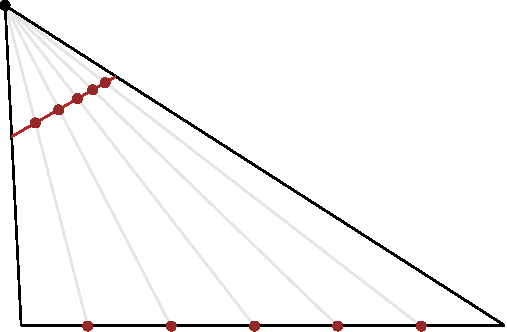
\includegraphics[scale=0.75]{figures/ProjectedGridVsWorldSpace.pdf}
%\label{fig:subfigprojgrid1}
%}
%\subbottom[Projected Grid]
%{
%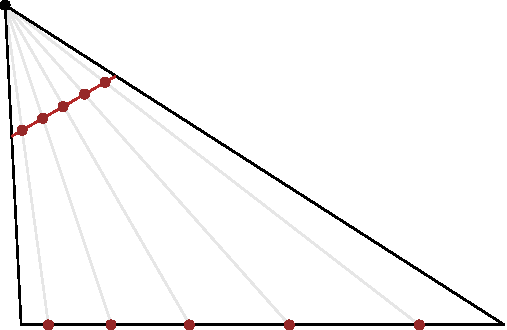
\includegraphics[scale=0.75]{figures/ProjectedGridUniform.pdf}
%\label{fig:subfigprojgrid2}
%}
%\caption{The image on the left shows an uniform grid in worldspace,
%its projection onto the image plane is not uniformly spaced though.
%The image on the right on the other hand depicts an uniform grid on
%the image plane and its associated non-uniform spaced worldspace
%positions.}
%\label{fig:projectedgrid}
%\end{figure}
%
%% The algorithm used for the projected grid can be broken down into the following
%% steps:
%% \begin{itemize}
%%  \item create a uniformly spaced grid orthogonal to the viewer using normalised
%% device coordinates
%%  \item transform the grid to worldspace
%%  \item project the grid onto the desired base plane
%%  \item apply height displacement
%%  \item run the grid through the rendering pipeline as usual
%% \end{itemize}
%
%\subsection{Coordinate Systems}
%\label{sec:coordinate_systems}
%Let $\mvec{x}$ be a vector representing the three dimensional carthesian
%world space coordinate of a vertex, then
%\begin{equation}
 %\mvec{w} = \transpose{(\mvecx{x}, \mvecy{x}, \mvecz{x}, 1)}
%\end{equation}
%where $\mvec{w}$ is a homogeneous world space coordinate of $\mvec{x}$.
%Let $\mmat{V}$ be the view matrix and $\mmat{P}$ the projection matrix, then
%\begin{equation}
%\label{eq:ws_to_cs}
 %\mvec{c} = \mmat{P} \mmat{V} \mvec{w}
%\end{equation}
%where $\mvec{c}$ is the \textit{clip space} coordinate of $\mvec{w}$. For $\mvec{c}$ to
%be inside the view frustum defined by $\mmat{P}$, $\mvec{c}$ is required to
%meet the following condition
%\begin{equation}
%\label{eq:cs_bounds}
 %\mvecx{c}, \mvecy{c}, \mvecz{c} \in \interval{-\mvecw{c}}{\mvecw{c}}
%\end{equation}
%where $\mvecw{c}$ is the homogeneous component of $\mvec{c}$. Next, clip space
%vertex $\mvec{c}$ is transformed by the \textit{perspective division} as follows
%\begin{equation}
%\label{eq:cs_to_ndc}
 %\mvec{n} = \frac{1}{\mvecw{c}}\transpose{(\mvecx{c}, \mvecy{c}, \mvecz{c})}
%\end{equation}
%where $\mvec{n}$ corresponds to the \textit{normalised device coordinate},
%\textit{NDC} in short, of $\mvec{c}$.
%%
%%
%\begin{figure}
%\centering
%\subbottom[View Frustum]
%{
%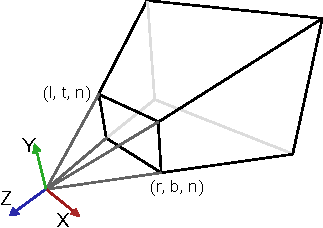
\includegraphics[width=0.4\textwidth]{figures/ProjectiveFrustum.pdf}
%\label{fig:subfig_proj_frustum}
%}
%\subbottom[Canonical view volume]
%{
%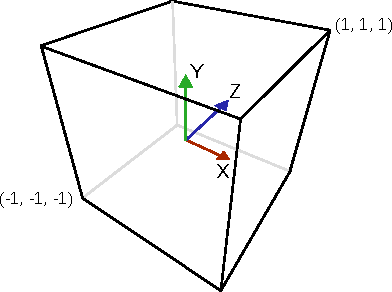
\includegraphics[width=0.4\textwidth]{figures/CanonicalCube.pdf}
%\label{fig:subfig_canonical_view_volume}
%}
%\caption{Left: An example view frustum in view space. Right: The same view frustum
%after applying projection and perspective division.}
%\label{fig:proj_frustum_ndc}
%\end{figure}
%%
%%
%As one can see, equations~\ref{eq:cs_bounds}
%and~\ref{eq:cs_to_ndc} imply
%\begin{equation}
%\label{eq:ndc_bounds}
 %\mvecx{n}, \mvecy{n}, \mvecz{n} \in \interval{-1}{1}
%\end{equation}
%which defines the space NDC reside in, namely the \textit{canonical view volume},
%see Figure~\ref{fig:proj_frustum_ndc}.\\
%
%
%The projected grid, on the other hand, starts inside the canonical view volume
%and needs to transform vertices back to world space. Let $\mvec{n}$ be the
%normalised device coordinate of a vertex, then
%\begin{equation}
%\label{eq:ndc_to_cs}
 %\mvec{c} = \transpose{(\mvecx{n}, \mvecy{n}, \mvecz{n}, 1)}
%\end{equation}
%where $\mvec{c}$ is a valid representation of $\mvec{n}$ in clip space. One may choose
%a value for $\mvecw{c}$ different from $1$, making it necessary to scale $\mvecx{n}$,
%$\mvecy{n}$ and $\mvecz{n}$ accordingly. Again, let $\mmat{V}$ be the view matrix and
%$\mmat{P}$ the projection matrix, then
%\begin{equation}
%\label{eq:cs_to_wsh}
 %\mvec{w} = \inverse{(\mmat{P} \mmat{V})} \mvec{c}
%\end{equation}
%where $\mvec{w}$ is a homogeneous world space coordinate of $\mvec{c}$. Conversion
%to three dimensional carthesian world space is accomplished as follows
%\begin{equation}
%\label{eq:wsh_to_ws}
 %\mvec{x} = \frac{1}{\mvecw{w}}\transpose{(\mvecx{w}, \mvecy{w}, \mvecz{w})}
%\end{equation}
%
%\subsection{Projection onto Plane}
%As noted before, the vertices of the projected grid are represented as normalised
%device coordinates. Assuming the plane the grid shall be projected on is specified
%in world space coordinates, the following steps need to be computed for each vertex:
%\begin{itemize}
 %\item Transform vertex from canonical view volume to world space
 %\item Setup vertex specific ray
 %\item Intersect ray with target plane to compute actual position
%\end{itemize}
%Step one is already covered by Section~\ref{sec:coordinate_systems}. Step two
%requires to setup a ray for each vertex, which implies both a position and a
%direction. The position we already have, but to create a direction we need two
%different positions. The solution is rather straightforward: let $\mvec{n}$ be
%a \textit{two-dimensional} vector representing the \textit{X} and \textit{Y}
%components of a position in normalised device coordinates, then
%\begin{align}
 %\mvec{a} & = (\mvecx{n}, \mvecy{n}, -1, 1)\\
 %\mvec{b} & = (\mvecx{n}, \mvecy{n}, +1, 1)
%\end{align}
%where $\mvec{a}$ corresponds to $\mvec{n}$ on the \textit{near plane} in clip space,
%and $\mvec{b}$ to $\mvec{n}$ on the \textit{far plane} in clip space. Let $\mvec{d}$
%and $\mvec{e}$ be the carthesian world space positions of $\mvec{a}$ and $\mvec{b}$
%respectively, then
%\begin{equation}
 %\label{eq:proj_grid_ray}
 %\mvec{p} = \mvec{d} + t(\mvec{e} - \mvec{d})
%\end{equation}
%where $\mvec{p}$ represents a ray starting at point $\mvec{d}$, pointing in direction
%$(\mvec{e} - \mvec{d})$ with variable parameter $t$ controlling the actual position on
%the ray.\\
%
%Step three is about intersecting ray $\mvec{p}$ resulting from step two with the target plane.
%We define the target plane using the \textit{Hesse normal form} as follows
%\begin{equation}
%\label{eq:proj_grid_plane}
 %\mvec{p}\transpose{\mvec{n}} - d = 0
%\end{equation}
%where $\mvec{n}$ is the plane's normal vector with unit length and $d$ the plane's distance
%from the origin. Next, we insert $\mvec{p}$ from equation~\ref{eq:proj_grid_ray}
%into equation~\ref{eq:proj_grid_plane}, resulting in
%%
%\begin{gather}
%\label{eq:plane_and_ray_intersection}
%(\mvec{d} + t(\mvec{e} - \mvec{d})\transpose{\mvec{n}} - d = 0\\
%\mvec{d}\transpose{\mvec{n}} + t(\mvec{e} - \mvec{d})\transpose{\mvec{n}} - d = 0\\
%\intertext{solve for $t$}
%t = \cfrac{d - \mvec{d}\transpose{\mvec{n}}}{(\mvec{e} - \mvec{d})\transpose{\mvec{n}}}
%\end{gather}
%%
%where $t$ in combination with equation~\ref{eq:proj_grid_ray} gives the point of intersection
%between the ray and the plane. In case $(\mvec{e} - \mvec{d})\transpose{\mvec{n}} = 0$,
%there is no point of intersection because the ray is parallel to the plane.
%
%\subsection{Projector}
%\fxnote*{JÖSSAS}{Backfiring, etc}

\section{Spectrum Synthesis}
\label{sec:spectrum_synthesis}
Recall Equation~\ref{eq:surface_elevation_discrete} in Chapter~\ref{sec:random_amplitudes},
where we defined surface elevation as follows:
\begin{equation}
\label{eq:dft_surface_elevation}
\eta(\mvec{x}, t) = 
\sum_{\mvec{k}}\frac{1}{\sqrt{2}}(\xi_r+\mathrm{i}\xi_i)
\sqrt{2\Theta(\mvec{k})\Delta k_x \Delta k_z} 
~\mathrm{e}^{-\mathrm{i}\omega(\mvec{k})t}
~\mathrm{e}^{\mathrm{i}\transpose{\mvec{k}}\mvec{x}}
\end{equation}
where $\xi_r$ and $\xi_i$ are random scalars drawn from the Standard Normal
Distribution. Both, the \wavevector domain $\mvec{k}$ and the
spatial domain $\mvec{x}$ are of resolution $N \times N$, where $N$ is a natural
number, and a power of two. The latter requirement is a concession to
the \FastFourierTransform algorithm, which works fastest at such
resolutions~\citep{Cooley:1965}.
Moreover, the spatial domain $\mvec{x}$ has an extent of $L \times L$, thus the
grid point spacing of the \wavevector domain is as follows:
\begin{equation*}
	\Delta k_x = \Delta k_z = \Delta k = \frac{2\pi}{L}
\end{equation*}
We may subsume part of Equation~\ref{eq:dft_surface_elevation} into the
following:
\begin{equation}
\label{eq:dft_h0_k}
h_0(\mvec{k}) = \frac{1}{\sqrt{2}}(\xi_r+\mathrm{i}\xi_i)\sqrt{2\Theta(\mvec{k})\Delta k_x \Delta k_z}
\end{equation}
where $h_0(\mvec{k})$ represents a random generated spectrum based on wave
energy spectrum $\Theta(\mvec{k})$. As long as the \wavevector domain and the
wave energy spectrum do not change, $h_0$ does not change either. Hence, it is
necessary to generate $h_0$ only once for a specific set of parameters such as
area, resolution, wind and fetch. As $h_0$ by itself has no notion of time,
we still need to take care of animation. Based on Equation~\ref{eq:dft_surface_elevation}
and \ref{eq:dft_h0_k} we may write:
\begin{equation}
\label{eq:dft_h_k_t}
h(\mvec{k},t) = h_0(\mvec{k})~\mathrm{e}^{-\mathrm{i}\omega(\mvec{k})t}
\end{equation}
where $t$ denotes the time.
Thus, $h$ as defined by Equation~\ref{eq:dft_h_k_t} has to be computed whenever
one requires a new keyframe for the animated ocean surface.
Equation~\ref{eq:dft_h0_k} on the other hand is only to be evaluated anew in
case parameters change, easing the computational workload by a
considerable margin.

\section{\DiscreteFourierTransform}
\label{sec:discrete_fourier_transform}
%
\newcommand{\ccellnum}[2]{\cellcolor{#1}\num{#2}}
\newcommand{\mcleft}[2]{\multicolumn{1}{!{\color{#1}\vline}S}{#2}}
\newcommand{\mcright}[2]{\multicolumn{1}{S !{\color{#1}\vline}}{#2}}
\newcommand{\mcleftright}[2]{\multicolumn{1}{!{\color{#1}\vline} S !{\color{#1}\vline}}{#2}}
\colorlet{Q1Color}{cyan!25}
\colorlet{Q2Color}{NavyBlue!50}
\colorlet{Q3Color}{violet!45}
\colorlet{Q4Color}{white}
\colorlet{Line1Color}{blue}
\colorlet{Line2Color}{black}
%
%
We compute surface elevation in the form of an \InvDiscreteFourierTransform as follows:
\begin{equation}
\label{eq:surface_elevation_h_k_t}
\eta(\mvec{x}, t) = \sum_{\mvec{k}}~h(\mvec{k},t)~\mathrm{e}^{\mathrm{i}\transpose{\mvec{k}}\mvec{x}}
\end{equation}
with
\begin{equation*}
\mvec{k} = (x,y)\in\{(\alpha\Delta k,\beta\Delta k)|
-\frac{N}{2}\leq\alpha<\frac{N}{2},-\frac{N}{2}<\beta\leq\frac{N}{2}\}
\end{equation*}
The \wavevector $\mvec{k} = (0,0)$ gives the location of the zero frequency component,
which encodes the average value of the signal in the spatial domain. In our specific
case that would be the mean surface elevation $\mathrm{E}[\eta] = 0$.
As one may read off the above definition of the \wavevector domain, the zero
frequency component is located near the center of the \wavevector domain,
where $\alpha=0$ and $\beta=0$. Actual implementations of the \InvFourierTransform,
such as FFTW~\citep{FFTW05}, expect the zero frequency component as the first element
i.e. at the upper left of the two-dimensional input array.
The \wavevector domain of such implementations is defined as follows:
\begin{equation*}
\mvec{k} = (x,y)\in\{(\alpha\Delta k,\beta\Delta k)|
0\leq\alpha,\beta<N\}
\end{equation*}
%
We know that the spectrum represents a periodic signal, therefore the spectrum
repeats itself at infinity in both directions. Hence, independent of where the
zero frequency is located inside the \wavevector domain, we may write:
%
\begin{align*}
 h(\mvec{k}(\alpha\Delta k,\beta\Delta k),t) = h(\mvec{k}((\alpha + lN)\Delta k, (\beta +mN)\Delta k),t) && l,m \in \mathbb{Z}
\end{align*}
%
%
\begin{figure}
\centering
%
\sisetup{
round-mode      = places,
round-precision = 1,
explicit-sign = +,
table-number-alignment=right
}
%
\begin{tabular}{cc}
	\subtop[]{
	\begin{tabular}{|SS|SS|}
	 \hline
	 \num{3.5886 + 0.0i}     & \num{0.5354 - 0.9111i}  & \num{-8.3447 + 0.0i}   & \num{0.5354 + 0.9111i} \\
	 \num{-2.0288 - 1.4957i} & \num{-0.2199 - 0.7443i} & \num{2.7433 + 2.5938i} & \num{0.1182 + 0.3465i} \\
	 \hline
	 \num{-0.5139 + 0.0i}    & \num{0.5448 - 0.2298i}  & \color{red}\num{0}     & \num{0.5448 + 0.2298i} \\
	 \num{-2.0288 + 1.4957i} & \num{0.1182 - 0.3465i}  & \num{2.7433 - 2.5938i} & \num{-0.2199 + 0.7443i} \\
	 \hline
	\end{tabular}
	\label{fig:spectrum:zfreq:center}
	}
	&
	\subtop[]{
	\begin{tabular}{cccc}
	 \hline
	 \multicolumn{2}{|c|}{\multirow{2}{*}{Q2}} & \multicolumn{2}{c|}{\multirow{2}{*}{Q1}} \\
	 \multicolumn{2}{|c|}{\multirow{2}{*}{}} & \multicolumn{2}{c|}{\multirow{2}{*}{}} \\
	 \hline
	 \multicolumn{2}{|c|}{\multirow{2}{*}{Q3}} & \multicolumn{2}{c|}{\multirow{2}{*}{\color{red}Q4}} \\
	 \multicolumn{2}{|c|}{\multirow{2}{*}{}} & \multicolumn{2}{c|}{\multirow{2}{*}{}} \\
	 \hline
	\end{tabular}
	\label{fig:zfreq:center}
	}
\end{tabular}
%
\begin{tabular}{c}
	\subtop[]{
	\begin{tabular}{cccccccc}
	 \hline
	 \multicolumn{2}{|c|}{\multirow{2}{*}{Q2}} & \multicolumn{2}{c|}{\multirow{2}{*}{Q1}} & \multicolumn{2}{c|}{\multirow{2}{*}{Q2}} & \multicolumn{2}{c|}{\multirow{2}{*}{Q1}} \\
	 \multicolumn{2}{|c|}{\multirow{2}{*}{}} & \multicolumn{2}{c|}{\multirow{2}{*}{}} & \multicolumn{2}{c|}{\multirow{2}{*}{}} & \multicolumn{2}{c|}{\multirow{2}{*}{}} \\
	 \hline
	 \multicolumn{2}{|c|}{\multirow{2}{*}{Q3}} & \multicolumn{2}{c|}{\multirow{2}{*}{\color{red}Q4}} & \multicolumn{2}{c|}{\multirow{2}{*}{Q3}} & \multicolumn{2}{c|}{\multirow{2}{*}{\color{red}Q4}} \\
	 \multicolumn{2}{|c|}{\multirow{2}{*}{}} & \multicolumn{2}{c|}{\multirow{2}{*}{}} & \multicolumn{2}{c|}{\multirow{2}{*}{}} & \multicolumn{2}{c|}{\multirow{2}{*}{}}\\
	 \hline
	 \multicolumn{2}{|c|}{\multirow{2}{*}{Q2}} & \multicolumn{2}{c|}{\multirow{2}{*}{Q1}} & \multicolumn{2}{c|}{\multirow{2}{*}{Q2}} & \multicolumn{2}{c|}{\multirow{2}{*}{Q1}} \\
	 \multicolumn{2}{|c|}{\multirow{2}{*}{}} & \multicolumn{2}{c|}{\multirow{2}{*}{}} & \multicolumn{2}{c|}{\multirow{2}{*}{}} & \multicolumn{2}{c|}{\multirow{2}{*}{}} \\
	 \hline
	 \multicolumn{2}{|c|}{\multirow{2}{*}{Q3}} & \multicolumn{2}{c|}{\multirow{2}{*}{\color{red}Q4}} & \multicolumn{2}{c|}{\multirow{2}{*}{Q3}} & \multicolumn{2}{c|}{\multirow{2}{*}{\color{red}Q4}} \\
	 \multicolumn{2}{|c|}{\multirow{2}{*}{}} & \multicolumn{2}{c|}{\multirow{2}{*}{}} & \multicolumn{2}{c|}{\multirow{2}{*}{}} & \multicolumn{2}{c|}{\multirow{2}{*}{}}\\
	 \hline
	\end{tabular}
	\label{fig:quadrants:periodic}
	}
\end{tabular}
%
\begin{tabular}{cc}
	\subtop[]{
	\begin{tabular}[b]{cccc}
	 \hline
	 \multicolumn{2}{|c|}{\multirow{2}{*}{\color{red}Q4}} & \multicolumn{2}{c|}{\multirow{2}{*}{Q3}} \\
	 \multicolumn{2}{|c|}{\multirow{2}{*}{}} & \multicolumn{2}{c|}{\multirow{2}{*}{}} \\
	 \hline
	 \multicolumn{2}{|c|}{\multirow{2}{*}{Q1}} & \multicolumn{2}{c|}{\multirow{2}{*}{Q2}} \\
	 \multicolumn{2}{|c|}{\multirow{2}{*}{}} & \multicolumn{2}{c|}{\multirow{2}{*}{}} \\
	 \hline
	\end{tabular}
	\label{fig:zfreq:upperleft}
	}
	&
	\subtop[]{
	\begin{tabular}{|SS|SS|}
	 \hline
	 \color{red}\num{0}     & \num{0.5448 + 0.2298i}  & \num{-0.5139 + 0.0i}    & \num{0.5448 - 0.2298i} \\
	 \num{2.7433 - 2.5938i} & \num{-0.2199 + 0.7443i} & \num{-2.0288 + 1.4957i} & \num{0.1182 - 0.3465i} \\
	 \hline
	 \num{-8.3447 + 0.0i}   & \num{0.5354 + 0.9111i}  & \num{3.5886 + 0.0i}     & \num{0.5354 - 0.9111i} \\
	 \num{2.7433 + 2.5938i} & \num{0.1182 + 0.3465i}  & \num{-2.0288 - 1.4957i} & \num{-0.2199 - 0.7443i} \\
	 \hline
	\end{tabular}
	\label{fig:spectrum:zfreq:upperleft}
	}
\end{tabular}
\caption{
\subcaptionref{fig:spectrum:zfreq:center} The spectrum of a real-valued signal ($N=4$),
the zero frequency component is highlighted in red.
\subcaptionref{fig:zfreq:center} Quadrant layout of the spectrum, the quadrant containig the zero frequency component is highlighted in red.
\subcaptionref{fig:quadrants:periodic} The signal is periodic, thus the spectrum is too. We may replicate the spectrum's quadrants along both dimensions, giving us alternative quadrant layouts to choose from.
\subcaptionref{fig:zfreq:upperleft} The quadrant layout we seek, where the zero frequency component is held by the quadrant at the origin. Compared to the
original layout, diagonally opposite quadrants have been swapped.
\subcaptionref{fig:spectrum:zfreq:upperleft} The spectrum is rearranged according to the modified quadrant layout, placing the zero frequency component at the origin.
}
\label{fig:quadrant:swapping}
\end{figure}
%
Figure~\ref{fig:quadrant:swapping} shows how we may use the periodical nature
of the spectrum to convert between the underlying layouts of the two different
\wavevector domains of interest.
%
%
\subsection{Hermitian Spectrum}
%https://www.cv.nrao.edu/course/astr534/FourierTransforms.html
%https://ccrma.stanford.edu/~jos/mdft/Even_Odd_Functions.html
%https://ccrma.stanford.edu/~jos/mdft/mdft.html
%https://web.eecs.umich.edu/~fessler/course/451/l/pdf/c5.pdf
The \FourierTransform of real-valued input is~\emph{hermitian} - the real part of the resulting spectrum
is an~\emph{even} function and the imaginary part is~\emph{odd}~\citep{book:bracewell2000fourier}.
A function $f(n)$ is said to be even if
$f(-n) = f(n)$. On the other hand, a function $f(n)$ is said to be odd if $f(-n) = -f(n)$,
with $f(0) = 0$. Let $\mathcal{F}(k)$ be the \FourierTransform of a real-valued function $f(n)$, then
the following is true:
\begin{equation}
\label{eq:dft_real_complex_conjugate}
 \mathcal{F}(-k) = \mathcal{F}(k)^*
\end{equation}
where $*$ denotes the complex conjugate operator. The relation is similar to a centrosymmetric one,
$\mathcal{F}(-k) = \mathcal{F}(k)$, with $\mathcal{F}(0)$ as a fixpoint at the center. The only
difference is the complex conjugation. \FourierTransform implementations such as FFTW~\citep{FFTW05}
take advantage of Equation~\ref{eq:dft_real_complex_conjugate} to be able to provide optimized
transform functionality for real-valued data. For example, for a forward \FourierTransform of real-valued data it is
necessary to compute only half of the spectrum, since the other half is implicitely given as the
complex conjugate of the first half. Likewise, for the \InvFourierTransform only half of the
spectrum is necessary, the other half is implicitely given. Such optimized transforms provide
gain in performance memory-wise, the spectrum's size is halved, as well as computation-wise, only
half the data is actually processed.
%
\begin{figure}
\footnotesize
\centering
\sisetup{
round-mode      = places,
round-precision = 1,
explicit-sign = +,
table-number-alignment=right
}
\setlength{\tabcolsep}{0pt}
\begin{tabular}{cc}
 \subtop[]{
	$\left(\begin{array}{lll}
	 a   &             b   & c   \\
	 d   & \color{red} e   & d^* \\
	 c^* &             b^* & a^* \\
	\end{array}\right)$
	\label{fig:symmetry:odd:layout}
 }
 &
 \subtop[]{
	$\left(\begin{array}{lll}
	 \num{-0.2199 - 0.7443i} & \num{2.7433 + 2.5938i} & \num{0.1182 + 0.3465i}  \\
	 \num{0.5448 - 0.2298i}  & \color{red}\num{0}     & \num{0.5448 + 0.2298i}  \\
	 \num{0.1182 - 0.3465i}  & \num{2.7433 - 2.5938i} & \num{-0.2199 + 0.7443i} \\
	\end{array}\right)$
	\label{fig:symmetry:odd:example}
 }
 \\
 \subtop[]{
	$\left(\begin{array}{lllll}
	a   & b   & c             & d   & e   \\
	f   & g   & h             & i   & j   \\
	k   & l   & \color{red} m & l^* & k^* \\
	j^* & i^* & h^*           & g^* & f^* \\
	e^* & d^* & c^*           & b^* & a^* \\
	\end{array}\right)$
	\label{fig:symmetry:even:layout}
 }
 &
 \subtop[]{
	$\left(\begin{array}{llll|l}
	 \num{3.5886 + 0.0i}     & \num{0.5354 - 0.9111i}  & \num{-8.3447 + 0.0i}   & \num{0.5354 + 0.9111i}  & \num{3.5886 + 0.0i} \\
	 \num{-2.0288 - 1.4957i} & \num{-0.2199 - 0.7443i} & \num{2.7433 + 2.5938i} & \num{0.1182 + 0.3465i}  & \num{-2.0288 - 1.4957i} \\
	 \num{-0.5139 + 0.0i}    & \num{0.5448 - 0.2298i}  & \color{red}\num{0}     & \num{0.5448 + 0.2298i}  & \num{-0.5139 + 0.0i} \\
	 \num{-2.0288 + 1.4957i} & \num{0.1182 - 0.3465i}  & \num{2.7433 - 2.5938i} & \num{-0.2199 + 0.7443i} & \num{-2.0288 + 1.4957i} \\
	 \hline
	 \num{3.5886 + 0.0i}     & \num{0.5354 - 0.9111i}  & \num{-8.3447 + 0.0i}   & \num{0.5354 + 0.9111i}  & \num{3.5886 + 0.0i} \\
	\end{array}\right)$
	\label{fig:symmetry:even:example}
 }
\end{tabular}
\caption{
The center element and the zero frequency component are highlighted in red respectively.
\subcaptionref{fig:symmetry:odd:layout} Hermitian matrix ($N=3$).
\subcaptionref{fig:symmetry:odd:example} Example spectrum matching the hermitian matrix layout.
\subcaptionref{fig:symmetry:even:layout} Hermitian matrix ($N=5$).
\subcaptionref{fig:symmetry:even:example} An even-sized spectrum ($N=4$), the elements of
the first row and column lack their complex conjugate counterparts.
Only after we replicate the spectrum until both its dimensions have an odd-numbered size ($N=5$),
we may find that for all elements of the spectrum there is a pair which satisfies the hermitian
condition $\mathcal{F}(-\mvec{k})=\mathcal{F}(\mvec{k})^*$.
%then for all elements of the spectrum there is a pair which satisfies the hermitian
%condition $\mathcal{F}(-\mvec{k})=\mathcal{F}(\mvec{k})^*$.
%An even-sized spectrum ($N=4$), which repeats itself in both directions, such as for all elements of the spectrum
%there is a pair which satisfies $\mathcal{F}(-\mvec{k})=\mathcal{F}(\mvec{k})^*$.
}
\label{fig:symmetry}
\end{figure}
%

Surface elevation $\eta$ is a real-valued function, therefore its spectrum must be hermitian,
too. Let $\mathcal{F}(\mvec{k})$ be the \FourierTransform of surface elevation $\eta$, then
we may write the hermitian property as follows:
\begin{equation}
\label{eq:h0_k_complex_conjugate}
 \mathcal{F}(-\mvec{k}) = \mathcal{F}(\mvec{k})^*
\end{equation}
where finding $\mathcal{F}(\mvec{k})^*$ for its counterpart $\mathcal{F}(-\mvec{k})$
has proven to be non-trivial for even-sized spectra.
Figure~\ref{fig:symmetry} shows that it is the periodic nature of the spectrum that
allows us to find matching complex conjugate pairs for all elements of an even-sized spectrum.

%Let the discretised wavevector domain be zero centered and of even size in both dimensions,
%then there is one row and one column of the spectrum which lacks
%matching complex conjugate elements inside said domain, see the example spectrum in Table~\ref{tab:spectrum_k_minusk}.
%Again, it is the periodic nature of the spectrum that gives us the solution. If we replicate
%the spectrum in both directions, we obtain an additional row and an additional column, which
%allows us to find matching pairs for all elements of the spectrum, see Table~\ref{tab:spectrum_k_minusk_border}.\\
\subsection{Hermitian Wave Spectrum}
The spectrum $h(\mvec{k},t)$ as we generate it with Equation~\ref{eq:dft_h_k_t} is~\emph{not}
hermitian for two reasons. First, the real-valued part of the spectrum, namely
the wave energy spectrum $\Theta(\mvec{k})$, would need to be an even function,
which is only the case if the directional spread employed by
the wave energy spectrum is centrosymmetric. Only two of the directional spreading functions
presented in this work are centrosymmetric, the Unified spectrum's and the Phillips spectrum's.
Second, each element of $h_0(\mvec{k})$ is generated in combination with a pair of random numbers,
which makes it close to impossible to end up with matching pairs $h_0(-\mvec{k})=h_0(\mvec{k})^*$.
As we would like to profit from the performance gains an optimized \InvFourierTransform
for real-valued functions offers, we are in need of a hermitian spectrum. Thus, we may
rewrite Equation~\ref{eq:dft_h_k_t} as follows:
%
\begin{equation}
\label{eq:dft_h_k_t_hermitian}
 h(\mvec{k}, t) =
 \frac{1}{2} h_0(\mvec{k})\mathrm{e}^{-\mathrm{i}\omega(\mvec{k})t}
 + \frac{1}{2} h_0(\mvec{-k})^*\mathrm{e}^{\mathrm{i}\omega(\mvec{k})t}
\end{equation}
%
which gives us a hermitian spectrum, independent both of the generated random numbers and 
whether the wave energy spectrum is an even function or not.

\emph{Note}: Surface elevation $\eta$ as computed by Equation~\ref{eq:surface_elevation_h_k_t}
gives the same results for Equation~\ref{eq:dft_h_k_t} and Equation~\ref{eq:dft_h_k_t_hermitian}.
Still, Equation~\ref{eq:dft_h_k_t} requires a standard \InvFourierTransform
with a complete complex-valued source spectrum and a
complex-valued result array of the same size. The real part of the result represents
the surface elevation, the imaginary part is to be discarded. Equation~\ref{eq:dft_h_k_t_hermitian},
on the other hand, allows for the aforementioned \InvFourierTransform
optimized for hermitian spectra, improving computation speed and memory usage
roughly by a factor of two~\citep{fftw:manual}.
%
\subsection{Combined \InvFourierTransform}
Given one hermitian spectrum, one may apply a specialized \InvFourierTransform
which requires only half of the actual spectrum. Given \emph{two} hermitian spectra,
one may combine them into a single spectrum and apply a standard \InvFourierTransform
to retrieve both real-valued signals at once \citep{fft:handbook}.
%The latter on the other hand allows for two different kinds of optimisation. We did discuss
%the first kind of optimisation already, a inverse Fourier Transform for real-valued
%functions which needs less memory and less time for the computation itself. The second kind
%of optimisation allows us to combine two inverse Fourier Transforms into one.
Let $a$ and $b$ be real-valued signals with identical underlying spatial domains.
Let us denote the \FourierTransform with $\mathcal{F}$, and the \InvFourierTransform
with $\mathcal{F}^{-1}$, then we may write:
%Let $\mathcal{F}(a)$ and $\mathcal{F}(b)$ be the Fourier Transforms of $a$ and
%$b$. Then we may write:
\begin{equation}
\label{eq:idft:combined}
c = \mathcal{F}^{-1}(\mathcal{F}(a)+\mathrm{i}\mathcal{F}(b))
\end{equation}
where $c$ is complex-valued. We are able to retrieve the original real-valued
signals from the real and imaginary components of $c$ respectively:
\begin{align*}
a &= \Re(c) & b &= \Im(c)
\end{align*}
%
We will make heavy use of this kind of optimization later on, because most
of our additional data required for rendering comes in pairs of hermitian spectra.
\subsection{Complex Conjugate Indices}
%
%To implement Equation~\ref{eq:dft_h_k_t_hermitian} we need to be able to retrieve
%matching pairs $(h_0(\mvec{k}),h_0(-\mvec{k}))$.
%Let us view $h_0$ as a two-dimensional array with size $N \times N$, where $N$ is an even number.
%Each element of $h_0$ is identified by a pair of indices $(i,j)$, with $0\leq i,j <N$. Then, for
%an element at index $(i,j)$, we may compute the index $(m,n)$ of the corresponding complex
%conjugate element as follows:
For implementation purposes, let us view the two-dimensional hermitian spectrum $h$
as a two-dimensional array with size $N \times N$.
Each element of $h$ is identified by a pair of indices $(i,j)$, with $0\leq i,j <N$. Then, for
an element at index $(i,j)$, we may compute the index $(m,n)$ of the corresponding complex
conjugate element as follows:
\begin{align}
\label{eq:complex:conjugate:indices}
m &= (N - i)\bmod N & n &= (N - j)\bmod N
\end{align}
We may write the hermitian property in terms of indices:
\begin{equation*}
 h(i,j) = h(m,n)^*
\end{equation*}
%
Moreover, let us view $h_0$ as a two-dimensional array with size $N \times N$,
with $h_0(\mvec{k}) = h_0(i,j)$. Then, we may employ Equation~\ref{eq:complex:conjugate:indices}
to retrieve $h_0(-\mvec{k})^*=h_0(m,n)^*$ as required by
Equation~\ref{eq:dft_h_k_t_hermitian}.
%

%
%Let $a(\mvec{k})$
%and $b(\mvec{k})$ be hermitian spectra with the same \wavevector domain $\mvec{k}$. Let $c(\mvec{x})$
%and $d(\mvec{x})$ be the corresponding real-valued signal of $a(\mvec{k})$ and $b(\mvec{k})$,
%then we may write:
%\begin{align}
%\label{eq:idft_combined}
 %e(\mvec{x}) &= \mathrm{IFT}(a(\mvec{k})+\mathrm{i}b(\mvec{k})) \\
 %c(\mvec{x}) &= \Re(e(\mvec{x})) \\
 %d(\mvec{x}) &= \Im(e(\mvec{x})) 
%\end{align}
%where $\mathrm{IFT}$ is shorthand for the standard inverse Fourier Transform.

%
\section{Slopes and Displacements}
\label{sec:slopes_and_displacements}
At this point we are able to compute surface elevation by application of the
\InvDiscreteFourierTransform on a spectrum we generate. For lighting
purposes we also need to find the surface's slope vectors to be able to compute
the surface's normal vectors. The most simple way to compute the slope is
through finite differences in the spatial domain of the surface. Such an
approach is efficient memory- and computation-wise, but may lack quality,
because it can be a poor approximation to the slope of waves with small
wavelengths~\citep{course:simulatingocean}. We are able to obtain more precise
slope vectors by employing \emph{spectral differentation}. Spectral
differentiation allows us to find the derivatives of a function via the
\FourierTransform~\citep{Trefethen:2000}.

First we will look at the more simple, one-dimensional case of spectral
differentiation. We reduce the spatial domain as well as the \wavevector domain
from beforehand to one dimension. Let $N$ be the resolution of the spatial
and \wavenumber domains, and $L$ the size of the spatial domain. Moreover, let
$\alpha \in \mathbb{N}$ with $-\frac{N}{2} \leq \alpha < \frac{N}{2}$,
let the spatial domain be $x \in \alpha \frac{L}{N}$, and let the \wavenumber
domain be $k \in \alpha \frac{2\pi}{L}$. Let $g(k)$ be the \DiscreteFourierTransform
of $f(x)$, then we may write the \InvDiscreteFourierTransform as follows:
\begin{equation*}
 f(x) = \sum_{k}g(k)~\mathrm{e}^{\mathrm{i}kx}
\end{equation*}
Note, that we omit the scaling factors involved in the standard \FourierTransform
because in the context of this work they are not needed. If we follow the
lead of the continuous \FourierTransform~\citep{Trefethen:2000},
then, in the discrete case, we may compute the $n$th derivative of $f(x)$ as follows:
\begin{equation}
\label{eq:dft:derivative:naive}
  \dod[n]{f(x)}{x} = \sum_{k}(\mathrm{i}k)^n~g(k)~\mathrm{e}^{\mathrm{i}kx}
\end{equation}
\citet{Johnson:2011} shows that Equation~\ref{eq:dft:derivative:naive} is not correct for odd $n$ in
combination with even $N$. For example, if $f(x)$ is a real function, then $g(k)$ is hermitian.
But $\mathrm{i}k~g(k)$ is~\emph{not} hermitian for even $N$, therefore the first
order derivative of $f(x)$ would end up a complex-valued function instead of a real-valued one.
To get correct results for all $n$ and $N$, we rewrite the above equation as follows:
\begin{align}
\label{eq:dft_derivative}
  \dod[n]{f(x)}{x} &= \sum_{k}d(k, n)~g(k)~\mathrm{e}^{\mathrm{i}kx} \\
\label{eq:dft_derivative_correction}
  d(k, n) &= \begin{cases}
                   0 &\text{if $n$ odd, and $N$ even, and $\abs{k}
= \frac{N}{2}\frac{2\pi}{L}$,} \\
                   (\mathrm{i}k)^n &\text{else.}
                   \end{cases}
\end{align}
%
\begin{figure}
 \centering
 \subtop[$\eta(\mvec{x},t)$]
 {
 \label{sfig:derivative_heights}
 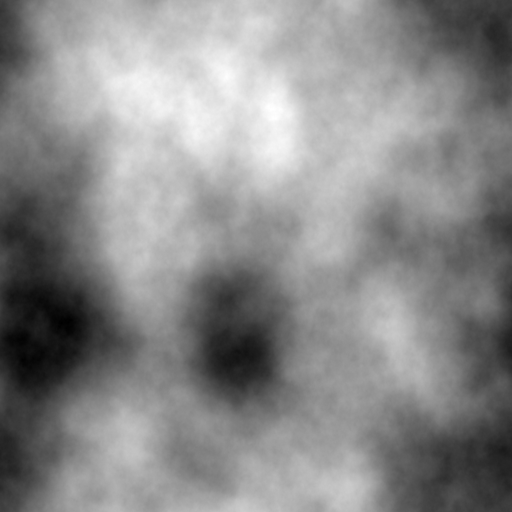
\includegraphics[scale=0.34]{figures/u_30_500km_heights.png}
 }
 \hfill
 \subtop[$\dpd{\eta(\mvec{x},t)}{x}$]
 {
 \label{sfig:derivative_x}
 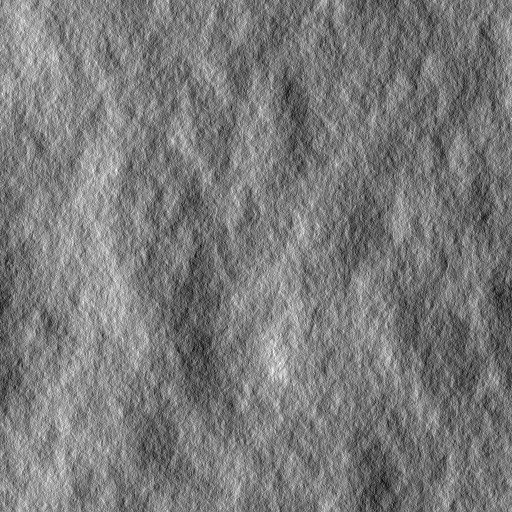
\includegraphics[scale=0.34]{figures/u_30_500km_gradient_x.png}
 }
 \hfill
 \subtop[$\dpd{\eta(\mvec{x},t)}{z}$]
 {
 \label{sfig:derivative_z}
 
\includegraphics[scale=0.34]{figures/u_30_500km_gradient_z.png}
 }
\caption{Brighter means larger values, darker means lower values.
\subcaptionref{sfig:derivative_heights} An example
surface wave height realization, displayed in greyscale (Unified spectrum, 
$U_{10}=30m\cdot s^{-1}$, $F=500km$). \subcaptionref{sfig:derivative_x} The 
first component of the slope vector. \subcaptionref{sfig:derivative_z} The 
second component of the slope vector.
}
\label{fig:derivatives}
\end{figure}
%
Now we may go back to the two-dimensional case, with our original two-dimensional
domains $\mvec{x}$ and $\mvec{k}$. The resolution of said domains is $N \times N$,
the size of the spatial domain is $L \times L$. Let $g(\mvec{k})$ be the
\DiscreteFourierTransform of $f(\mvec{x})$, then we may write the
\InvDiscreteFourierTransform in two dimensions as follows:
\begin{equation*}
 f(\mvec{x}) = \sum_{\mvec{k}}g(\mvec{k})~\mathrm{e}^{\mathrm{i}\transpose{\mvec{k}}\mvec{x}}
\end{equation*}
Based on Equation~\ref{eq:dft_derivative}, and by reusing Equation~\ref{eq:dft_derivative_correction}
because $N$ and $L$ are equal for both dimensions, we find the derivatives of $f(\mvec{x})$:
\begin{equation}
\label{eq:dft_derivates_2d}
 \dmd{f(\mvec{x})}{n+m}{x}{n}{z}{m} = \sum_{\mvec{k}}d(k_{x}, n)d(k_{z}, m)~g(\mvec{k})~\mathrm{e}^{\mathrm{i}\transpose{\mvec{k}}\mvec{x}}
\end{equation}
where $x$ and $z$ denote the two components of vector $\mvec{x}$, and $k_x$ and $k_z$ 
the two components of \wavevector $\mvec{k}$ respectively.
As we need to find the surface slope vector, we need to compute 
the surface elevation's first order partial derivatives. Given surface 
elevation $\eta(\mvec{x},t)$, we obtain the two-dimensional surface slope 
vector $\mvec{s}$ as follows:
\begin{equation}
\label{eq:dft_slope_2d}
 \mvec{s}(\mvec{x},t) = \left[\dpd{\eta(\mvec{x},t)}{x}, \dpd{\eta(\mvec{x},t)}{z}\right]
\end{equation}
We leave it as an exercise for the reader to substitute the terms $\eta(\mvec{x},t)$
and $h(\mvec{k},t)$ into Equation~\ref{eq:dft_derivates_2d} to be able to
compute the surface slope vector as given in Equation~\ref{eq:dft_slope_2d}.
Figure~\ref{fig:derivatives} depicts an example instance of surface 
elevation $\eta$ as well as its associated slopes in greyscale.
%One may notice that Figure~\ref{sfig:derivative_heights}, without prior
%knowledge, is not  recognizable as a wave heightfield. The wave heightfield's
%gradients in Figure~\ref{sfig:derivative_x} and \subcaptionref{sfig:derivative_z},
%on the other hand, are more easily identified as water waves by the human eye.

The two spectra which constitute the surface slope vector in the \wavevector domain
are hermitian. Therefore we are able to apply the optimisation from
Equation~\ref{eq:idft:combined} which allows us to combine both spectra into one,
obtaining both components of the surface slope vector with just one \InvFourierTransform.
%
\subsection{Normal Vectors}
%
In this work we employ a right-handed Carthesian coordinate system where the positive
Y-axis points in the opposite direction of earth's gravity.
The two-dimensional surface slope vector lies in the XZ-plane of the world space
coordinate system. Based on the surface slope vector we may find the unit
length surface normal vector $\mvec{n}$ as follows:
\begin{equation*}
 \mvec{n} = \frac{(-s_x, 1, -s_z)}{\norm{(-s_x, 1, -s_z)}}
\end{equation*}
where $s_x$ and $s_z$ denote the two components of slope vector $\mvec{s}$
as obtained by Equation~\ref{eq:dft_slope_2d}.
%
\subsection{Displacements}
\label{sec:displacements}
%
\begin{figure}
 \centering
 \subtop[$\eta(\mvec{x},t)$]
 {
 \label{sfig:displacement_heights}
 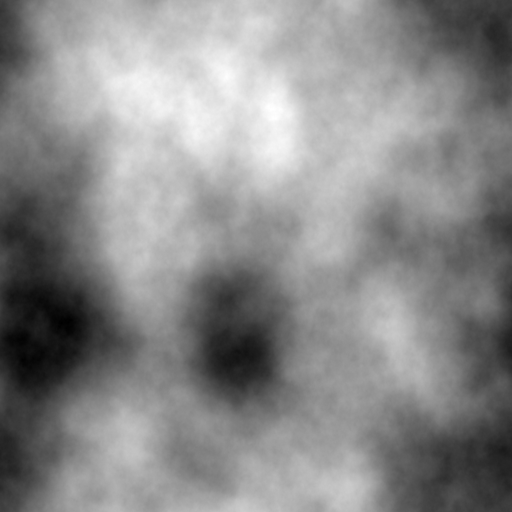
\includegraphics[scale=0.34]{figures/u_30_500km_heights.png}
 }
 \hfill
 \subtop[$D_x(\mvec{x},t)$]
 {
 \label{sfig:displacement_x}
 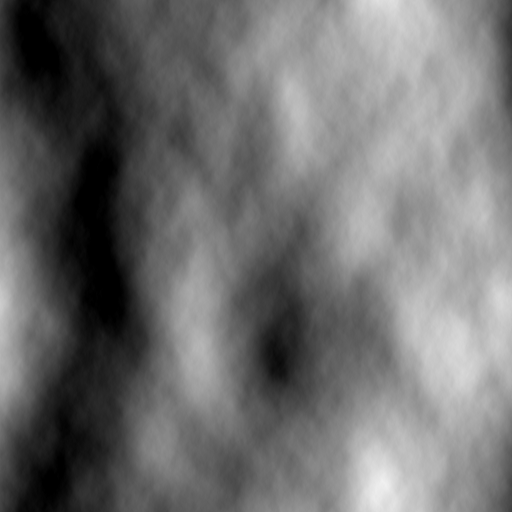
\includegraphics[scale=0.34]{figures/u_30_500km_displacement_x.png}
 }
 \hfill
 \subtop[$D_z(\mvec{x},t)$]
 {
 \label{sfig:displacement_z}
 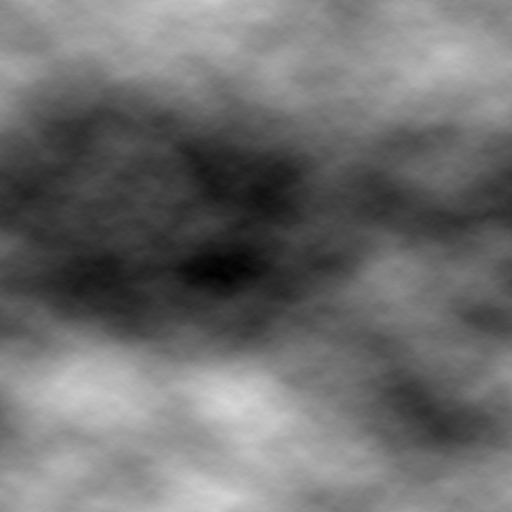
\includegraphics[scale=0.34]{figures/u_30_500km_displacement_z.png}
 }
\caption{
Brighter means larger values, darker means lower values.
\subcaptionref{sfig:displacement_heights} An example surface wave height
realization, displayed in greyscale (Unified spectrum, $U_{10}=30m\cdot s^{-1}$, $F=500km$).
\subcaptionref{sfig:displacement_x} The first component of the displacement vector.
\subcaptionref{sfig:displacement_z} The second component of the displacement vector.
}
\label{fig:displacements}
\end{figure}
%
The waves generated with the methods presented up to now tend to have rounded peaks and troughs,
which is typical for fair weather conditions. But we also would like to be able to synthesize waves
matching poor weather conditions, such as strong winds or even storms. During such weather, ocean waves
are sharply peaked at their tops and flattened at the bottoms. \citet{course:simulatingocean}
describes a method based on the \FourierTransform to produce such choppy waves. The concept is simple: displace
the grid points of the spatial domain in the XZ-plane, with the displacement varying locally with the waves.
Note that the displacement is a two-dimensional vector, therefore we end up computing a vector field.
Similar to spectral differentiation, we compute an \InvFourierTransform of the spectrum $h$,
where the latter is modified by an additional term. We may write the displacement vector field as follows:
\begin{equation}
%\label{eq:dft_displacement}
 \mvec{D}(\mvec{x},t) = \left[D_x(\mvec{x},t), D_z(\mvec{x},t)\right]
\end{equation}
with
\begin{align}
\label{eq:displacement_x} D_x(\mvec{x},t) &= \sum_{\mvec{k}}d(k_x, 
k)~h(\mvec{k},t)~\mathrm{e}^{\mathrm{i}\transpose{\mvec{k}}\mvec{x}} \\
\label{eq:displacement_z} D_z(\mvec{x},t) &= \sum_{\mvec{k}}d(k_z, 
k)~h(\mvec{k},t)~\mathrm{e}^{\mathrm{i}\transpose{\mvec{k}}\mvec{x}} \\
%\label{eq:dft_displacement_correction}
 d(l, k) &= \begin{cases}
             0 &\text{if $N$ even, and $k = 0$ or $\abs{l} = 
\frac{N}{2}\frac{2\pi}{L}$,} \\
             -\mathrm{i}\frac{l}{k} &\text{else.}
            \end{cases}
\end{align}
where the term $d(l, k)$, in addition to make sure the resulting spectrum is 
hermitian, also avoids a division by zero at $k = 0$. 
Figure~\ref{fig:displacements} shows an example instance of surface elevation 
$\eta$ as well as its associated displacements in greyscale.
Because the spectra on the righthand side of Equations~\ref{eq:displacement_x} 
and~\ref{eq:displacement_z} are hermitian, we are again able to apply 
Equation~\ref{eq:idft:combined} and obtain both components of the displacement 
vector field with just one \InvFourierTransform.

% The grid points of the spatial domain are two-dimensional, $\mvec{x} = [x_x, 
% x_y]$, and lie in the XZ-plane of our three dimensional space. Embedded into 
% three dimensional space, they represent the ocean plane at rest, $\mvec{p} = 
% [x_x, 0, x_y]$. We may add surface elevation $\eta$ $[x_x, \eta(\mvec{x},t), 
% x_y]$

Given grid point $\mvec{x} = (x,z)$, time $t$ and surface elevation $\eta(\mvec{x},t)$, 
we may write the corresponding three dimensional, vertically displaced vertex 
coordinate as follows:
\begin{equation}
 \mvec{v}(\mvec{x},t) = \begin{bmatrix}x\\ \eta(\mvec{x},t)\\ z\end{bmatrix} 
\end{equation}
With displacement vector $\mvec{D}(\mvec{x},t)$ at hand, according to 
\citet{course:simulatingocean} we may compute the three dimensional,
vertically and horizontally displaced vertex coordinate as follows:
\begin{equation}
\label{eq:displacement_gridpoints}
 \mvec{w}(\mvec{x},t) =
 \begin{bmatrix}
  x + u D_x(\mvec{x},t)\\ 
  \eta(\mvec{x},t)\\
  z + u D_z(\mvec{x},t)
 \end{bmatrix}
\end{equation}
where $u\in\mathbb{R}$ is a user-controlled parameter to scale the importance of the
displacement vector. We have found that the above formula is correct as long as
$u \leq 0$, otherwise the effect is the opposite of what we want to achieve.
Looking at Equation~\ref{eq:displacement_gridpoints},
one can see that it is not the wave heights that are altered, but instead the grid
points on the XZ-plane are transformed based on the spatial structure of the
height field. This particular transformation accomplishes the effects we sought:
the waves' peaks are sharpened and the waves' valleys are broadened.
%
\begin{figure}
\centering
\begin{tikzpicture}
\begin{axis}[
	width=\textwidth,
	height=4cm,
    legend style={draw=none},
    %legend/.append style={nodes={right}},
	legend pos= south west,
	legend cell align=left,
	xtick = {-50, -40, -30, -20, -10, 0, 10, 20, 30, 40, 50},
	ytick = {-0.5, 0, 0.5},
    xlabel={Spatial domain coordinate~$x$~(\si{\metre})},
    ylabel={Surface height~$\eta$~(\si{\metre})},
	%enlarge y limits = 0.2,
]
\addplot[
    color=red,
    solid,
	]
    table [
		col sep=comma, 
		x expr=\thisrowno{0},
		y expr=\thisrowno{2},
	]
	{figures/u_30_500km_x_dx_h.dat};
\addlegendentry{$x$}
\addplot[
    color=blue,
    solid,
	]
    table [
		col sep=comma, 
		x expr=\thisrowno{0} - 3*\thisrowno{1},
		y expr=\thisrowno{2},
	]
	{figures/u_30_500km_x_dx_h.dat};
\addlegendentry{$x + u D_x(x,t)$}
\end{axis}
\end{tikzpicture}
\caption{Red: the original wave profile. Blue: the displaced wave profile, note 
the steep tops and the flattened valleys ($u = -3$).}
\label{fig:grid_displaced}
\end{figure}
%
Figure~\ref{fig:grid_displaced} shows two profiles of the wave height along one 
direction, where one profile uses displaced coordinates, while the other does 
not.
%
\subsection{Slopes after Displacement}
%
Based on Figure~\ref{fig:grid_displaced} one may see that the application 
of displacements does not only alter the underlying grid points, but as a 
direct consequence the surface's slopes, too. Hence, we need to adjust our 
computation of the slope vector to the new circumstances. Given surface 
elevation $\eta(\mvec{x},t)$, displacement vector $\mvec{D}(\mvec{x},t)$,
and grid point transformation $\mvec{x} + u\mvec{D}(\mvec{x},t)$,
according to \citet[private communication]{article:whitecaps} we obtain the
two-dimensional surface slope $\mvec{s}$ as follows:
\begin{equation}
\mvec{s}(\mvec{x},t) = \left[\frac{\dpd{\eta(\mvec{x},t)}{x}}{1 + u 
\dpd{D_x(\mvec{x},t)}{x}}, \frac{\dpd{\eta(\mvec{x},t)}{z}}{1 + u 
\dpd{D_z(\mvec{x},t)}{z}}\right]
\end{equation}
where $u$ is the displacement scale parameter. Now, in addition
to surface height $\eta$, displacement vector $\mvec{D}$, and the slopes of $\eta$,
we also need to compute a partial derivative of $D_x$ and $D_z$ each.
Again, we may compute the latter two by means of spectral
differentiation, see Equation~\ref{eq:dft_derivates_2d}. Morever, we are again
able to apply the optimisation from Equation~\ref{eq:idft:combined} which allows
us to transform the spectra of the two partial derivatives as one.
%
\subsection{Self-Intersections}
\label{sec:self_intersections}
%
\begin{figure}
\centering
\begin{tikzpicture}[
	spy using outlines={circle, magnification=5, connect spies}
]
\begin{axis}[
	width=\textwidth,
	height=4cm,
    legend style={draw=none},
    %legend/.append style={nodes={right}},
	legend pos= south west,
	legend cell align=left,
	xtick = {-50, -40, -30, -20, -10, 0, 10, 20, 30, 40, 50},
	ytick = {-0.5, 0, 0.5},
    xlabel={Spatial domain coordinate~$x$~($\text{m}$)},
    ylabel={Surface height~$\eta$~($\text{m}$)},
	axis lines = left,
	%enlarge y limits = 0.3,
]
\addplot[
    color=red!15!white,
    solid,
	forget plot
	]
    table [
		col sep=comma, 
		x expr=\thisrowno{0},
		y expr=\thisrowno{2},
	]
	{figures/u_30_500km_x_dx_h.dat};
%\addlegendentry{$x$}
\addplot[
    color=blue,
    solid,
	]
    table [
		col sep=comma, 
		x expr=\thisrowno{0} - 7.5*\thisrowno{1},
		y expr=\thisrowno{2},
	]
	{figures/u_30_500km_x_dx_h.dat};
\addlegendentry{$x + u D_x(x,t)$}
\coordinate (spypoint1) at (axis cs:-44,0.45);
\coordinate (magnifyglass1) at (axis cs:-44,2);

\coordinate (spypoint2) at (axis cs:-16,0);
\coordinate (magnifyglass2) at (axis cs:-16,2);

\coordinate (spypoint3) at (axis cs:5.5,-0.425);
\coordinate (magnifyglass3) at (axis cs:5.5,2);

\coordinate (spypoint4) at (axis cs:48.25,0.7);
\coordinate (magnifyglass4) at (axis cs:48.25,2);

\end{axis}
\spy [black, size=2cm] on (spypoint1) in node[fill=white] at (magnifyglass1);
\spy [black, size=2cm] on (spypoint2) in node[fill=white] at (magnifyglass2);
\spy [black, size=2cm] on (spypoint3) in node[fill=white] at (magnifyglass3);
\spy [black, size=2cm] on (spypoint4) in node[fill=white] at (magnifyglass4);
\end{tikzpicture}
\caption{
Background: the original wave profile.
Foreground: the displaced wave profile, with some of the self-intersections
highlighted. We chose a large displacement scaling parameter ($u=-7.5$) to
better emphasize the effect of self-intersection.
%The wave profile from Figure~\ref{fig:grid_displaced}, but with 
%displacement scaling parameter $u=-7.5$ to better emphasize the effect of 
%self-intersection. The non-displaced wave profile is shown in the background.
}
\label{fig:grid_displaced_self_intersection}
\end{figure}
%
The method by \citet{course:simulatingocean} we use to generate 
choppy waves is not devoid of drawbacks.
As shown in Figure~\ref{fig:grid_displaced_self_intersection}, some of the
displacement vectors we compute may be large enough to cause the displaced
geometry to self-intersect. Near the top of some 
waves the surface actually passes through itself, and as a consequence inverts, 
with the surface normal pointing inwards instead of outwards. We may get rid of 
this undesired side-effect in a rather simple way: reduce the magnitude of 
displacement scaling parameter $u$.
On the other hand, \citeauthor{course:simulatingocean} suggests that we use
said self-intersections to our advantage, because they may be able to signal
the breaking of waves, as well as the production of foam and spray. Hence, we
need to be able to test for such self-intersections in an efficient manner.
\citeauthor{course:simulatingocean} recommends to 
compute the determinant of the~\emph{Jacobian matrix} of the transformation 
from grid point $\mvec{x}$ to displaced grid point 
$\mvec{x}+u\mvec{D}(\mvec{x},t)$. Based on the determinant we may decide if 
self-intersection is taking place.
%
%
\begin{figure}
\centering
\begin{tikzpicture}
\begin{axis}[
  width=\textwidth,
  height=10cm,
  legend style={draw=none},
  %legend/.append style={nodes={right}},
  legend pos= south west,
  legend cell align=left,
  xtick = {-50, -40, -30, -20, -10, 0, 10, 20, 30, 40, 50},
  %ytick = {-0.5, 0, 0.5},
  xlabel={Spatial domain coordinate~$x$~($\text{m}$)},
  ylabel={Surface height~$\eta$~($\text{m}$)},
  axis lines = left,
  %enlarge y limits = 0.3,
]
\addplot[
  color=ForestGreen,
  dotted,
  ]
  table [
    col sep=comma, 
    x expr=\thisrowno{0} - 7.5*\thisrowno{1},
    y expr=(1-7.5*\thisrowno{3})*(1-7.5*\thisrowno{6}) - 
    ((-7.5*\thisrowno{5}) * (-7.5*\thisrowno{4})),
  ]
  {figures/u_30_500km_x_dx_h_dxx_dxz_dzx_dzz.dat};
%\addplot[
  %color=red!15!white,
  %solid,
  %forget plot
  %]
  %table [
    %col sep=comma, 
    %x expr=\thisrowno{0},
    %y expr=\thisrowno{2},
    %]
  %{figures/u_30_500km_x_dx_h_dxx_dxz_dzx_dzz.dat};
%\addlegendentry{$x$}
\addplot[
  color=blue,
  solid,
  ]
  table [
    col sep=comma, 
    x expr=\thisrowno{0} - 7.5*\thisrowno{1},
    y expr=\thisrowno{2},
    ]
  {figures/u_30_500km_x_dx_h_dxx_dxz_dzx_dzz.dat};
%\addlegendentry{$x + u D_x(x,t)$}
\addplot[
  color=black,
  solid,
  ]
  table [
    col sep=comma, 
    x expr=\thisrowno{0},
    y expr=0,
    ]
  {figures/u_30_500km_x_dx_h_dxx_dxz_dzx_dzz.dat};
%\addlegendentry{$x + u D_x(x,t)$}
\end{axis}
\end{tikzpicture}
\caption{Blue: the displaced wave profile ($u = -7.5$). Green: the Jacobian 
determinant. Note, that each instance of surface self-intersection is 
accompanied by negative Jacobian determinants.}
\label{fig:grid_displaced_j}
\end{figure}
%
First, we need the Jacobian matrix of the grid point transformation 
$\mvec{g}(\mvec{x},t)=\mvec{x}+u\mvec{D}(\mvec{x},t)$. The Jacobian matrix is 
the matrix of all first order partial derivatives of a vector valued function. 
As grid point transformation $\mvec{g}$ maps from $\mathbb{R}^2$ to 
$\mathbb{R}^2$, the Jacobian matrix is $2\times 2$ in size. Let $\mvec{J}$ be 
the Jacobian matrix of transformation $\mvec{g}$, then we may write:
%
\begin{equation*}
 \label{eq:jacobian_of_displacement}
 \mvec{J}(\mvec{x},t) =
 \begin{bmatrix}
 J_{xx} & J_{xz} \\
 J_{zx} & J_{zz}
 \end{bmatrix}
 =
 \begin{bmatrix}
   1 + u\dpd{D_x(\mvec{x},t)}{x} & u\dpd{D_x(\mvec{x},t)}{z} \\[1em]
   u\dpd{D_z(\mvec{x},t)}{x} & 1 + u\dpd{D_z(\mvec{x},t)}{z}
 \end{bmatrix}
\end{equation*}
Next, we compute the determinant of the Jacobian matrix:
\begin{equation*}
 det(\mvec{J}(\mvec{x},t)) = J_{xx}J_{zz}-J_{zx}J_{xz}
\end{equation*}
%
If the Jacobian determinant at $\mvec{x}$ is positive, then $\mvec{g}$ 
preserves orientation near $\mvec{x}$. If it is negative, $\mvec{g}$ reverses 
orientation. We are interested in the latter case, because wherever the 
surface self-intersects, it actually folds back on itself via a loop, and a 
loop requires a reversal of orientation. Figure~\ref{fig:grid_displaced_j} 
depicts a displaced surface, as well as the corresponding Jacobian 
determinants. One can see that wherever the surface self-intersects, the 
Jacobian determinant is negative.

% \begin{tabular}{lS[table-format = 3]S[table-format = 3.2]}
% \toprule
%   \textbf{Bus} & \multicolumn{2}{c}{\textbf{Bus Load (MVA)}} \\
%                & {Real} & {Complex} \\
%   \midrule
%   b1 &  50 &  30.99 \\
%   b2 & 170 & 105.35 \\
%   b3 & 200 & 123.94 \\
%   b4 & 150 &  49.58 \\
%   \bottomrule
% \end{tabular}

\section{Level of Detail}
\label{sec:level_of_detail}
The core of our ocean model are the spectra discussed in 
Section~\ref{sec:wave_spectra}. We sample the spectra in 
frequency space to obtain vertical and horizontal displacements produced by 
ocean waves. Because the sampling process is done by means of a \DiscreteFourierTransform,
the resulting data can be seamlessly tiled on the ocean surface. 
However, tiling a single perturbation pattern either leads to repetitive 
artifacts if the tile's footprint in world space is small, or to lack of detail 
if the tile's footprint in world space is large. We chose to tackle these 
issues like \citet{misc:oceanlightingfft} and \citet{article:whitecaps},
which compute not only one perturbation pattern, but a set of perturbation
patterns of different size, which are then superimposed over each other.
%, where each pattern is different in size and therefore may sample
%a different part of the spectrum.
Although this approach is not able to entirely remove the tiling artifacts from
the wave field, it is still able to reduce periodicity to the least common
multiple of the pattern periods.
Moreover, as the \wavenumber ranges of the different patterns complement each
other, we are able to extend the sum of waves to include shorter wavelengths,
even as far as into the gravity-capillary wave domain.
%each pattern samples a different part of the spectrum, we are able
%to extend the sum of waves to include shorter wavelengths, even as far as into
%the gravity-capillary wave domain.
Thus, given a sufficient number of patterns,
we may be able to consistently reproduce small-scale detail for closeups of the
water surface.
In practice, up to four different perturbation patterns may suffice to obtain
satisfactory results \citep{article:whitecaps}.

Since we position this work in the context of real-time rendering,
we need to make sure that the accumulated cost of pattern data synthesis
does not prevent us to keep real-time framerates. 
Thus, we may extend the level-of-detail approach by \citet{misc:oceanlightingfft} and
\citet{article:whitecaps} with a multi-resolution scheme, where specific pattern
datasets, such as surface elevation and displacements, are generated at a lower
resolution than the other datasets. 
%Consequentially, the potential reduction of computational workload is exclusively
%dependent on the actual difference between the two resolutions.
%We may conclude that, based on the number of patterns and the resolution(s) of pattern data,
%we are able to strike a well-adjusted balance between model detail and computational workload.

%Second, we reduce the amount of spectral data to transform. We achieve the
%latter by improving upon the level-of-detail approach by \citet{misc:oceanlightingfft}
%and \citet{article:whitecaps} with a multi-resolution scheme, where surface
%elevation and displacements are generated at a lower resolution
%than their respective first-order derivates.

In the remainder of this section we upgrade our equations to handle more than
one perturbation pattern, we explain how to parametrize the different pattern
periods to be able to reduce tiling artifacts as well as reproduce as much
detail as possible, and last we discuss our multi-resolution approach.
%
\subsection{Equations}
At this point, one perturbation pattern consists of surface
elevation $\eta$, displacement vector $\mvec{D}$, the slopes of $\eta$,
and the first order partial derivatives of $\mvec{D}$.
Because we compute the surface
displacements as a sum of waves, it is straightforward to extend our
computations to incorporate not just one perturbation pattern, but a set of
patterns. Let $l \in \mathbb{N}^+$ represent the number of different patterns,
then we may compute the combined surface elevation as follows:
\begin{equation}
 y(\mvec{x},t) = \sum\limits_{i=0}^{l-1}\eta_i(\mvec{x},t)
\end{equation}
In lockstep with the above we compute the slope of the combined surface elevation:
\begin{equation}
 \mvec{s}(\mvec{x},t) = \left[\dpd{y(\mvec{x},t)}{x},\dpd{y(\mvec{x},t)}{z}\right]
 = \left[\sum\limits_i \dpd{\eta_i(\mvec{x},t)}{x}, \sum\limits_i \dpd{\eta_i(\mvec{x},t)}{z}\right]
\end{equation}
Furthermore, we may extend the horizontal grid point transformation required by
the choppy wave algorithm to the following:
\begin{equation}
\mvec{g}(\mvec{x},t) = \mvec{x}+\sum\limits_{i=0}^{l-1}u_i\mvec{D}_i(\mvec{x},t) 
\end{equation}
Thus, we may write the slope of the combined displaced surface elevation as follows:
\begin{equation}
\mvec{s}(\mvec{x},t) = \left[\frac{\sum\limits_i \dpd{\eta_i(\mvec{x},t)}{x}}{1 
+ \sum\limits_i u_i \dpd{D_{xi}(\mvec{x},t)}{x}}, \frac{\sum\limits_i 
\dpd{\eta_i(\mvec{x},t)}{z}}{1 + \sum\limits_i 
u_i\dpd{D_{zi}(\mvec{x},t)}{z}}\right]
\end{equation}
Given the new grid point transformation, we are in need of the corresponding
Jacobian matrix to be able to locate surface self-intersections. We may write:
\begin{equation}
\label{eq:jacobian_of_displacement_multi}
 \mvec{J}(\mvec{x},t) =
 \begin{bmatrix}
 J_{xx} & J_{xz} \\
 J_{zx} & J_{zz}
 \end{bmatrix}
 =
 \begin{bmatrix}
   1 + \sum\limits_i u_i\dpd{D_{xi}(\mvec{x},t)}{x} & \sum\limits_i u_i\dpd{D_{xi}(\mvec{x},t)}{z} \\[1em]
   \sum\limits_i u_i\dpd{D_{zi}(\mvec{x},t)}{x} & 1 + \sum\limits_i u_i\dpd{D_{zi}(\mvec{x},t)}{z}
 \end{bmatrix}
\end{equation}
%
One can see that in case the number of patterns equals one, the new equations
simply fall back to the original ones.
%
\subsection{Tiling}
As mentioned before, we aim to reduce tiling artifacts as much as possible
by superimposing a set of patterns of different size \citep{misc:oceanlightingfft}.
To be able to do so we require a minimum of two patterns: a large one which defines
the general shape of the ocean surface, and a small one for closeup detail.
\citet{Bridson:2015} argues that if one takes such an approach to reduce
periodicity, then it would be best for the different pattern sizes to be related
to each other by an irrational number, because only then one may be able to
generate an aperiodic signal. In short, given pattern size $L$, then we may
obtain the next tile size as $\alpha L$, where $\alpha$ is an irrational number.
\citeauthor{Bridson:2015} goes even further, and states that it would
be best to choose scaling factor $\alpha$ based on the~\emph{golden ratio}
$\varphi = (1 + \sqrt{5})/2$.
Thus, we devised a simple automatism where the user specifies the size of the
largest pattern, and then each subsequent pattern is automatically shrunk in
size by factor $f$, with $f \in \{\varphi^{-1}, 1 - \varphi^{-1}\}$. The two
choices for $f$ represent the lengths of the line segments one obtains if a
line of length one is split in two based on the golden ratio.
Let $L$ be the size of the largest pattern, then we may compute sizes $L_i$ of
the successive patterns as follows:
\begin{align}
\label{eq:pattern_size_i}
 L_i = f^{i} L && 0 < i < l
\end{align}
where $l$ is the number of patterns.

Although the above gives us an aperiodic signal (not accounting for numerical
accuracy), we are not able to completely eliminate periodicity. In some cases
the human observer is still able to recognize that the underlying dominant
structure, as represented by the largest pattern, appears multiple times.
Still, we have found Equation~\ref{eq:pattern_size_i} to be a surprisingly
simple as well as adequate solution to the issue at hand.
Should one deem it necessary, he or she may always choose pattern
sizes via a different mechanism, based on other irrational numbers, or even by
hand as \citeauthor{article:whitecaps} did.

\subsection{\Wavenumber Range}
%
We employ multiple patterns of different size to reduce tiling artifacts. A
convenient side-effect of such an approach is that the combination of multiple
patterns includes more distinct \wavenumbers into the sum of waves than a single
pattern does. However, before we elaborate on the effect of
multiple patterns on \wavenumber sampling, we may concern ourselves with the
\wavenumbers sampled by a single pattern.
Recall that both, the spatial domain and the \wavevector domain, are defined
entirely by size $L$ and resolution $N$. The minimal, non-zero \wavenumber
representable by the \wavevector domain is $k = 2\pi/L$, it depends only on
size. Moreover, the distance between subsequent
sample points in both dimensions is defined as $\Delta k = 2\pi/L$.
Hence, $\Delta k$ depends only on size. Therefore, by choosing size $L$, we do
not only define the minimal \wavenumber we are able to sample, but also
how densely we are able to sample the spectrum. The largest \wavenumber contained
in the \wavevector domain is $k = \sqrt{2}\pi N/L$. So, given size $L$,
resolution $N$ defines how large the \wavenumbers are allowed to grow, giving us
an upper limit of the \wavenumbers involved in the sum of waves. In short, with
size $L$ and resolution $N$ specified for a pattern, we are able to compute the
pattern's \wavenumber range and sampling density.
%
\begin{figure}
\centering
\begin{tikzpicture}
\begin{groupplot}[
	group style={
		columns=4,
		rows=1,
		xlabels at=edge bottom,
		ylabels at=edge left,
	},
    xlabel={$k_d$},
    ylabel=\empty,
	width=0.3\textwidth,
	axis x line=bottom,
%	ymin = 0,
%	ymax = 0.001,
	]
\nextgroupplot[
	ytick=\empty,
	axis y line=none,
	title = {(a) $L=100m$},
	xmin = 0,
	xmax = 1.4,
	]
\addplot[
  color=red,
  %mark color=blue,
  %mark=halfdiamond*,
  fill,
  fill opacity=0.2,
  ]
  table [
    col sep=comma, 
  ]
  {figures/sampling_res_12_area_100.dat} \closedcycle;
\addplot[
  ycomb,
  color=red,
  ]
  table [
    col sep=comma, 
  ]
  {figures/sampling_res_12_area_100.dat};
\nextgroupplot[
	ytick=\empty,
	axis y line=none,
	title = {(b) $L=50m$},
	xmin = 0,
	xmax = 1.4,
	]
\addplot[
  color=red,
  fill,
  fill opacity=0.2,
  ]
  table [
    col sep=comma, 
  ]
  {figures/sampling_res_12_area_50.dat} \closedcycle;
\addplot[
  ycomb,
  color=red,
  ]
  table [
    col sep=comma, 
  ]
  {figures/sampling_res_12_area_50.dat};
\nextgroupplot[
	ytick=\empty,
	axis y line=none,
	title = {(c) $N=12$},
	xmin = 0,
	xmax = 1.5,
	]
\addplot[
  color=blue,
  fill,
  fill opacity=0.2,
  ]
  table [
    col sep=comma, 
  ]
  {figures/sampling_area_100_res_12.dat} \closedcycle;
\addplot[
  ycomb,
  color=blue,
  ]
  table [
    col sep=comma, 
  ]
  {figures/sampling_area_100_res_12.dat};
\nextgroupplot[
	ytick=\empty,
	axis y line=none,
	title = {(d) $N=24$},
	xmin = 0,
	xmax = 1.5,
	]
\addplot[
  color=blue,
  fill,
  fill opacity=0.2,
  ]
  table [
    col sep=comma, 
  ]
  {figures/sampling_area_100_res_24.dat} \closedcycle;
\addplot[
  ycomb,
  color=blue,
  ]
  table [
    col sep=comma, 
  ]
  {figures/sampling_area_100_res_24.dat};
\end{groupplot}
\end{tikzpicture}
\caption{Red: Equal resolution, $N=12$, different size $L$.
%Both, (a) and (b), consist of the same number of samples.
(a) covers a smaller \wavenumber range
than (b) because the former employs a smaller distance $\Delta k = 2\pi/L$
between consecutive sample points.
Blue: Equal size, $L=\SI{100}{\metre}$, different resolution $N$. The distance between
consecutive sample points is equivalent in (c) and (d). (d) covers a larger
\wavenumber range because it contains more samples than (c).}
\label{fig:sampling_area_vs_res}
\end{figure}
%

Let $k_d$ be a set of distinct \wavenumbers based on parameters $L$ and $N$.
With the \wavenumber set $k_d$ at hand we may sample a one-dimensional
\wavenumber spectrum. Figure~\ref{fig:sampling_area_vs_res} depicts a set of
reconstructions of the same one-dimensional \wavenumber spectrum, where one
can see the effects of size $L$ and resolution $N$ on the \wavenumber set $k_d$,
and thus on the reconstructed spectrum.

%\citet{Bridson:2015} argues that if one wants to reduce periodicity by
%superimposing two tiling patterns with different size, then one should employ
%irrational numbers as scaling factors. In short, given pattern size $L$, then
%we may obtain the next tile size as $\alpha L$, where $\alpha$ is an irrational
%number. \citeauthor{Bridson:2015} goes even further, and states that it would
%be best to choose scaling factor $\alpha$ based on the~\emph{golden ratio}
%$\varphi = (1 + \sqrt{5})/2$.

\subsection{\Wavenumber Sampling}
\begin{figure}[p]
\centering
\begin{tikzpicture}
\begin{groupplot}[
	group style={
		columns=4,
		rows=2,
		%xlabels at=edge bottom,
		xlabels at=all,
		ylabels at=edge left,
	},
    xlabel={$k$},
    ylabel=\empty,
	width=0.3\textwidth,
	axis x line=bottom,
%	ymin = 0,
%	ymax = 0.001,
	]
\nextgroupplot[
	ytick=\empty,
	axis y line=none,
	]
\addplot[
  color=red,
  fill,
  fill opacity=0.2,
  unbounded coords=discard,
  ]
  table [
    col sep=comma, 
  ]
  {figures/sampling_scale_03_lod_1.dat} \closedcycle;
\nextgroupplot[
	ytick=\empty,
	axis y line=none,
	]
\addplot[
  color=blue,
  fill,
  fill opacity=0.2,
  unbounded coords=discard,
  ]
  table [
    col sep=comma, 
  ]
  {figures/sampling_scale_03_lod_2.dat} \closedcycle;
\nextgroupplot[
	ytick=\empty,
	axis y line=none,
	]
\addplot[
  color=green,
  fill,
  fill opacity=0.2,
  unbounded coords=discard,
  ]
  table [
    col sep=comma, 
  ]
  {figures/sampling_scale_03_lod_3.dat} \closedcycle;
\nextgroupplot[
	ytick=\empty,
	axis y line=none,
	]
\addplot[
  color=orange,
  fill,
  fill opacity=0.2,
  unbounded coords=discard,
  ]
  table [
    col sep=comma, 
  ]
  {figures/sampling_scale_03_lod_4.dat} \closedcycle;
\nextgroupplot[
	ytick=\empty,
	axis y line=none,
	]
\addplot[
  color=red,
  fill,
  fill opacity=0.2,
  unbounded coords=discard,
  ]
  table [
    col sep=comma, 
  ]
  {figures/sampling_scale_06_lod_1.dat} \closedcycle;
\nextgroupplot[
	ytick=\empty,
	axis y line=none,
	]
\addplot[
  color=blue,
  fill,
  fill opacity=0.2,
  unbounded coords=discard,
  ]
  table [
    col sep=comma, 
  ]
  {figures/sampling_scale_06_lod_2.dat} \closedcycle;
\nextgroupplot[
	ytick=\empty,
	axis y line=none,
	]
\addplot[
  color=green,
  fill,
  fill opacity=0.2,
  unbounded coords=discard,
  ]
  table [
    col sep=comma, 
  ]
  {figures/sampling_scale_06_lod_3.dat} \closedcycle;
\nextgroupplot[
	ytick=\empty,
	axis y line=none,
	]
\addplot[
  color=orange,
  fill,
  fill opacity=0.2,
  unbounded coords=discard,
  ]
  table [
    col sep=comma, 
  ]
  {figures/sampling_scale_06_lod_4.dat} \closedcycle;
\end{groupplot}
\end{tikzpicture}
\caption{
A one-dimensional \wavenumber spectrum reconstructed at resolution $N = 128$,
with initial pattern size $L = \SI{1750}{\metre}$, and subsequent, reduced
pattern sizes obtained by Equation~\ref{eq:pattern_size_i}.
Top row: pattern sizes are reduced by factor $f=1-\varphi^{-1}$.
Bottom row: pattern sizes are reduced by factor $f = \varphi^{-1}$.
Note the difference in \wavenumber range between top and bottom row.
}
\label{fig:sampling_pattern_size_reduction}
\end{figure}
%
%
\begin{figure}[p]
\centering
\begin{tikzpicture}
\begin{groupplot}[
	group style={
		columns=3,
		rows=2,
		%xlabels at=edge bottom,
		xlabels at=all,
		ylabels at=edge left,
	},
    xlabel={$k$},
    ylabel=\empty,
	width=0.35\textwidth,
	axis x line=bottom,
%	ymin = 0,
%	ymax = 0.001,
	]
\nextgroupplot[
	ytick=\empty,
	axis y line=none,
	]
\addplot[
  color=red,
  fill,
  fill opacity=0.2,
  ]
  table [
    col sep=comma, 
  ]
  {figures/sampling_scale_03_lod_1.dat} \closedcycle;
\addplot[
  color=blue,
  fill,
  fill opacity=0.2,
  ]
  table [
    col sep=comma, 
  ]
  {figures/sampling_scale_03_lod_2_capped.dat} \closedcycle;
\nextgroupplot[
	ytick=\empty,
	axis y line=none,
	]
\addplot[
  color=red,
  fill,
  fill opacity=0.2,
  ]
  table [
    col sep=comma, 
  ]
  {figures/sampling_scale_03_lod_1.dat} \closedcycle;
\addplot[
  color=blue,
  fill,
  fill opacity=0.2,
  ]
  table [
    col sep=comma, 
  ]
  {figures/sampling_scale_03_lod_2_capped.dat} \closedcycle;
\addplot[
  color=green,
  fill,
  fill opacity=0.2,
  ]
  table [
    col sep=comma, 
  ]
  {figures/sampling_scale_03_lod_3_capped.dat} \closedcycle;
\nextgroupplot[
	ytick=\empty,
	axis y line=none,
	]
\addplot[
  color=red,
  fill,
  fill opacity=0.2,
  ]
  table [
    col sep=comma, 
  ]
  {figures/sampling_scale_03_lod_1.dat} \closedcycle;
\addplot[
  color=blue,
  fill,
  fill opacity=0.2,
  ]
  table [
    col sep=comma, 
  ]
  {figures/sampling_scale_03_lod_2_capped.dat} \closedcycle;
\addplot[
  color=green,
  fill,
  fill opacity=0.2,
  ]
  table [
    col sep=comma, 
  ]
  {figures/sampling_scale_03_lod_3_capped.dat} \closedcycle;
\addplot[
  color=orange,
  fill,
  fill opacity=0.2,
  ]
  table [
    col sep=comma, 
  ]
  {figures/sampling_scale_03_lod_4_capped.dat} \closedcycle;
\nextgroupplot[
	ytick=\empty,
	axis y line=none,
	]
\addplot[
  color=red,
  fill,
  fill opacity=0.2,
  ]
  table [
    col sep=comma, 
  ]
  {figures/sampling_scale_06_lod_1.dat} \closedcycle;
\addplot[
  color=blue,
  fill,
  fill opacity=0.2,
  ]
  table [
    col sep=comma, 
  ]
  {figures/sampling_scale_06_lod_2_capped.dat} \closedcycle;
\nextgroupplot[
	ytick=\empty,
	axis y line=none,
	]
\addplot[
  color=red,
  fill,
  fill opacity=0.2,
  ]
  table [
    col sep=comma, 
  ]
  {figures/sampling_scale_06_lod_1.dat} \closedcycle;
\addplot[
  color=blue,
  fill,
  fill opacity=0.2,
  ]
  table [
    col sep=comma, 
  ]
  {figures/sampling_scale_06_lod_2_capped.dat} \closedcycle;
\addplot[
  color=green,
  fill,
  fill opacity=0.2,
  ]
  table [
    col sep=comma, 
  ]
  {figures/sampling_scale_06_lod_3_capped.dat} \closedcycle;
\nextgroupplot[
	ytick=\empty,
	axis y line=none,
	]
\addplot[
  color=red,
  fill,
  fill opacity=0.2,
  ]
  table [
    col sep=comma, 
  ]
  {figures/sampling_scale_06_lod_1.dat} \closedcycle;
\addplot[
  color=blue,
  fill,
  fill opacity=0.2,
  ]
  table [
    col sep=comma, 
  ]
  {figures/sampling_scale_06_lod_2_capped.dat} \closedcycle;
\addplot[
  color=green,
  fill,
  fill opacity=0.2,
  ]
  table [
    col sep=comma, 
  ]
  {figures/sampling_scale_06_lod_3_capped.dat} \closedcycle;
\addplot[
  color=orange,
  fill,
  fill opacity=0.2,
  ]
  table [
    col sep=comma, 
  ]
  {figures/sampling_scale_06_lod_4_capped.dat} \closedcycle;
\end{groupplot}
\end{tikzpicture}
\caption{
Gradual assembly of the reconstructed spectra from Figure
\ref{fig:sampling_pattern_size_reduction} into one coherent spectrum.
The transition from data from one spectrum to data from the next
spectrum takes place at the maximum \wavenumber of the spectrum with the
smaller \wavenumber range.
}
\label{fig:sampling_pattern_assembly}
\end{figure}
%
% For us to generate a believable, as well as visually pleasing ocean surface, we
% are required to include into our sum of waves a finite set of distinct
% \wavenumbers such that it is representative of the whole energy.
We have seen in Figure~\ref{fig:sampling_area_vs_res} that if we generate only
one pattern, based on size and resolution, we either sparsely sample inside a
large \wavenumber range, or we densely sample inside a small \wavenumber range.
If, on the other hand, we generate multiple patterns of differing size, then
the patterns' \wavenumbers ranges complement each other. Thus, we are able
to sample a significantly larger \wavenumber range at a varying, but reasonable
density. Varying, because the sampling density changes from pattern to pattern
based on pattern size.
The enlarged \wavenumber range may contain short \wavelengths up to, and
including the gravity-capillary wave domain, which represents waves with a
length from one to several centimeters. With such short waves involved in the
sum of waves we have the opportunity to reproduce sufficient detail for
close-ups of the water surface. Still, we need to make sure to set a lower
limit of $\lambda_{min} = \SI{1.73}{\centi\metre}$ for the \wavelengths included
by any of the patterns, because for waves shorter than $\lambda_{min}$ gravity is
replaced by surface tension as the major restoring force, making them
capillary waves. The latter are not modeled correctly by any of the wave
spectra presented in Section~\ref{sec:wave_spectra}, because those wave spectra
concern themselves exclusively with gravity waves.

%Given the enlarged \wavenumber range, we are able to
%include shorter \wavelengths into the sum of waves, allowing us to reproduce
%sufficient detail for close-ups of the water surface.

Figure~\ref{fig:sampling_pattern_size_reduction} shows that the \wavenumber
ranges of the different patterns are partially overlapping,
therefore we need to make sure to sample each \wavenumber only once.
Thus, if the spectrum of one pattern already covers a specific
\wavenumber range, a second spectrum covering parts or the entirety of that same
range, has to be zeroed in the region of overlap. Moreover, it is the spectrum
of the pattern with larger size that should have precedence, as it has higher
sampling density.
Figure~\ref{fig:sampling_pattern_assembly} shows the assembly of the overlapping
spectra from Figure~\ref{fig:sampling_pattern_size_reduction} into one coherent
spectrum. We get the best sampling density, if the transition from data from
one spectrum to data from the next spectrum takes place at the maximum
\wavenumber of the spectrum with the smaller \wavenumber range.
%Care has to be taken not to sample the same part of the spectrum multiple times.
%FIXME: Double negative. Not doing so, would imply including the same \wavenumber(s) multiple times in the
%sum of waves. Thus, if the spectrum of one pattern already covers a specific
%\wavenumber range, a second spectrum covering parts or the entirety of that same
%range, has to be zeroed in the region of overlap.
%Figure~\ref{fig:sampling_pattern_assembly} shows the assembly of the overlapping
%spectra from Figure~\ref{fig:sampling_pattern_size_reduction} into one coherent
%spectrum. The transition from data from one spectrum to data from the next
%spectrum always happens at the maximum \wavenumber of the spectrum with the
%smaller \wavenumber range.
%include a larger number of distinct \wavenumbers into the sum of waves
%compared to a single pattern.
%The
%former results in a poor reconstruction of a larger part of the spectrum, the
%latter in a better reconstruction of a smaller part of the spectrum, but
%possibly missing other relevant parts of the spectrum. 
%Fortunately, we already generate more than one pattern 
%Thus, if we generate more
%than one pattern, then we may be able to sample as many distinct \wavenumbers as
%possible. As explained before, each pattern has its specific \wavenumber range
%based on pattern resolution and pattern size.
%For simplicity's sake our implementation uses the same resolution for a dataset across all patterns.
%

\emph{Note}: The typical profile of a one-dimensional \wavenumber spectrum suggests
that it would be beneficial to employ an adaptive sampling scheme which allows
for tight sampling in the low \wavenumber range, especially near the peak
\wavenumber, and sparse sampling in the high \wavenumber range
\citep{article:frechot2007}. Because we employ a \DiscreteFourierTransform to
compute the sum of waves, we are subject to its constraints. One of
those constraints is that the spacing between successive coordinates is constant,
namely $\Delta k$. Hence, in combination with a \DiscreteFourierTransform, we
are not allowed to employ a sampling scheme where $\Delta k$ changes dependent
on which part of the \wavenumber profile is being sampled.
%
%
%For us to generate a believable, as well as visually pleasing ocean surface, we
%are required to include into our sum of waves a finite set of \wavenumbers such
%that it is representative of the whole energy. If we generate only one pattern,
%based on size and resolution, we either sparsely sample inside a large
%\wavenumber range, or we densely sample inside a small \wavenumber range. The
%former results in a poor reconstruction of a larger part of the spectrum, the
%latter in a better reconstruction of a smaller part of the spectrum, but
%possibly missing other relevant parts of the spectrum. Thus, we generate more
%than one pattern, where the goal is to sample as many distinct
%\wavenumbers as possible.
%
%\subsection{Pattern Sizes}
%%
%We would like to sample the spectrum at as many \wavenumbers as possible,
%therefore we need to minimize overlap of the \wavenumber ranges of different
%patterns. Because our implementation shares the same dataset resolution(s) $N$
%across all patterns, we are forced to focus on pattern size $L$ to reduce
%\wavenumber overlap.
%%In our implementation each dataset shares the same resolution across
%%all patterns, therefore we focus on pattern size to reduce \wavenumber overlap.
%We need at least one large pattern size, to avoid repetitive artifacts as much
%as possible, and one small pattern size for closeup detail.
%\citet{Bridson:2015} argues that if one wants to reduce periodicity by
%superimposing two tiling patterns with different size, then one should employ
%irrational numbers as scaling factors. In short, given pattern size $L$, then
%we may obtain the next tile size as $\alpha L$, where $\alpha$ is an irrational
%number. \citeauthor{Bridson:2015} goes even further, and states that it would
%be best to choose scaling factor $\alpha$ based on the~\emph{golden ratio}
%$\varphi = (1 + \sqrt{5})/2$.
%
%
%In addition, we have to make sure that the different sizes are not integral
%multiples of each other, otherwise the surface may seem repetitive at a smaller
%scale than expected. 
%FIXME: irrational number~\citet{Bridson:2015}
%We chose to tackle both requirements by
%employing multiples based on the golden ratio $\varphi = (1 + \sqrt{5})/2$. The
%user sets the largest desired pattern size, each following pattern size is
%reduced by the same multiplicative factor $f$, where $f \in \{\varphi^{-1},
%1 - \varphi^{-1}\}$.
%
%
%In case we choose $f = 1-\varphi^{-1} \approx 0.382$, the combined patterns
%allow for tight sampling around the spectral peak as well as in the high
%\wavenumber range. Hence, the sum of waves includes both, large wavelengths which
%give the overall surface its shape, and small wavelengths for close-up detail.
%The drawback of this choice are the smaller pattern sizes, which results in
%repetitive artifacts at a smaller scale than expected. In case we choose
%$f = \varphi^{-1} \approx 0.618$, the combined patterns allow for even more
%tight sampling around the spectral peak, but missing most of the energy in the
%high \wavenumber range. Thus, it is the large wavelengths we are able to
%reconstruct, but missing close-up detail. On the other hand, we have less issues
%with repetitive artifacts. The two rows in Figure~\ref{fig:sampling_pattern_size_reduction}
%depict the reconstructions of one and the same spectrum, based on patterns with
%the same resolution $N$, but initial size $L$ reduced by the two different
%factors.
%
\subsection{Multiple Resolutions}
%
%
\begin{figure}[p]
\centering
\begin{tikzpicture}
\begin{groupplot}[
	group style={
		columns=4,
		rows=2,
		%xlabels at=edge bottom,
		xlabels at=all,
		ylabels at=edge left,
	},
    xlabel={$k$},
    ylabel=\empty,
	width=0.3\textwidth,
	axis x line=bottom,
%	ymin = 0,
%	ymax = 0.001,
	]
\nextgroupplot[
	ytick=\empty,
	axis y line=none,
	xmin = 0,
	xmax = 0.46,
	]
\addplot[
  color=red!20!white,
  ]
  table [
    col sep=comma, 
  ]
  {figures/sampling_multires_scale_06_res_128_8_lod_1.dat};
\addplot[
  ycomb,
  color=red,
  ]
  table [
    col sep=comma, 
  ]
  {figures/sampling_multires_scale_06_res_64_8_lod_1.dat};
\addplot[
  color=red,
  %draw=red,
  fill,
  fill opacity=0.2,
  ]
  table [
    col sep=comma, 
  ]
  {figures/sampling_multires_scale_06_res_64_8_lod_1.dat} \closedcycle;
\nextgroupplot[
	ytick=\empty,
	axis y line=none,
	xmin = 0,
	xmax = 0.74,
	]
\addplot[
  color=blue!20!white,
  ]
  table [
    col sep=comma, 
  ]
  {figures/sampling_multires_scale_06_res_128_8_lod_2.dat};
\addplot[
  ycomb,
  color=blue,
  ]
  table [
    col sep=comma, 
  ]
  {figures/sampling_multires_scale_06_res_64_8_lod_2.dat};
\addplot[
  color=blue,
  fill,
  fill opacity=0.2,
  ]
  table [
    col sep=comma, 
  ]
  {figures/sampling_multires_scale_06_res_64_8_lod_2.dat} \closedcycle;
\nextgroupplot[
	ytick=\empty,
	axis y line=none,
	xmin = 0,
	xmax = 1.2,
	]
\addplot[
  color=green!20!white,
  ]
  table [
    col sep=comma, 
  ]
  {figures/sampling_multires_scale_06_res_128_8_lod_3.dat};
\addplot[
  ycomb,
  color=green,
  ]
  table [
    col sep=comma, 
  ]
  {figures/sampling_multires_scale_06_res_64_8_lod_3.dat};
\addplot[
  color=green,
  fill,
  fill opacity=0.2,
  ]
  table [
    col sep=comma, 
  ]
  {figures/sampling_multires_scale_06_res_64_8_lod_3.dat} \closedcycle;
\nextgroupplot[
	ytick=\empty,
	axis y line=none,
	xmin = 0,
	xmax = 1.94,
	]
\addplot[
  color=yellow!20!white,
  ]
  table [
    col sep=comma, 
  ]
  {figures/sampling_multires_scale_06_res_128_8_lod_4.dat};
\addplot[
  ycomb,
  color=yellow,
  ]
  table [
    col sep=comma, 
  ]
  {figures/sampling_multires_scale_06_res_64_8_lod_4.dat};
\addplot[
  color=yellow,
  fill,
  fill opacity=0.2,
  ]
  table [
    col sep=comma, 
  ]
  {figures/sampling_multires_scale_06_res_64_8_lod_4.dat} \closedcycle;
\nextgroupplot[
	ytick=\empty,
	axis y line=none,
	xmin = 0,
	xmax = 0.46,
	]
\addplot[
  color=red,
  fill,
  fill opacity=0.2,
  ]
  table [
    col sep=comma, 
  ]
  {figures/sampling_multires_scale_06_res_128_8_lod_1.dat} \closedcycle;
\addplot[
  ycomb,
  color=red,
  ]
  table [
    col sep=comma, 
  ]
  {figures/sampling_multires_scale_06_res_128_8_lod_1.dat};
\nextgroupplot[
	ytick=\empty,
	axis y line=none,
	xmin = 0,
	xmax = 0.74,
	]
\addplot[
  color=blue,
  fill,
  fill opacity=0.2,
  ]
  table [
    col sep=comma, 
  ]
  {figures/sampling_multires_scale_06_res_128_8_lod_2.dat} \closedcycle;
\addplot[
  ycomb,
  color=blue,
  ]
  table [
    col sep=comma, 
  ]
  {figures/sampling_multires_scale_06_res_128_8_lod_2.dat};
\nextgroupplot[
	ytick=\empty,
	axis y line=none,
	xmin = 0,
	xmax = 1.2,
	]
\addplot[
  color=green,
  fill,
  fill opacity=0.2,
  ]
  table [
    col sep=comma, 
  ]
  {figures/sampling_multires_scale_06_res_128_8_lod_3.dat} \closedcycle;
\addplot[
  ycomb,
  color=green,
  ]
  table [
    col sep=comma, 
  ]
  {figures/sampling_multires_scale_06_res_128_8_lod_3.dat};
\nextgroupplot[
	ytick=\empty,
	axis y line=none,
	xmin = 0,
	xmax = 1.94,
	]
\addplot[
  color=yellow,
  fill,
  fill opacity=0.2,
  ]
  table [
    col sep=comma, 
  ]
  {figures/sampling_multires_scale_06_res_128_8_lod_4.dat} \closedcycle;
\addplot[
  ycomb,
  color=yellow,
  ]
  table [
    col sep=comma, 
  ]
  {figures/sampling_multires_scale_06_res_128_8_lod_4.dat};
\end{groupplot}
\end{tikzpicture}
\caption{A one-dimensional \wavenumber spectrum as reconstructed by multiple
patterns of different size.
Pattern size $L$ shrinks with each consecutive column, it follows that both rows have
matching distances between successive samples. Top row uses resolution $N = 8$,
whereas bottom row uses $N = 16$. One can see that each reconstruction in top
row is a subset of the reconstruction in bottom row.
%Top and bottom row use equal pattern sizes, it follows that both rows have matching distances between
%subsequent samples. Top row employs half the resolution of bottom row, therefore
%each of its reconstructions is equal the left half of the correspondig
%reconstruction in bottom row.
}
\label{fig:sampling_different_resolutions}
\end{figure}
%
%
Recall, that one perturbation pattern consists of surface elevation $\eta$,
displacement vector $\mvec{D}$, the slopes of $\eta$, and the first order
partial derivatives of $\mvec{D}$. Moreover, we have a set of such patterns. The
computational load to synthesize all the cumulated pattern data has proven to be
substantial. To improve upon the status quo, we chose to implement an approach
common in computer graphics: augment low-resolution geometry with high-resolution
surface information to generate detailed lighting. For our specific case, that
means we may synthesize vertical and horizontal displacements at a lower
resolution than the associated derivatives.
%
%
Given pattern size $L$, grid point spacing $\Delta k = 2\pi/L$, pattern
resolutions $N_h,N_l \in \mathbb{N}$ with $N_l < N_h$, then we may define the
two following \wavevector domains:
%
\begin{align}
\mvec{h} = (k_x,k_z)~&\in~\{(\alpha\Delta k,\beta\Delta k)|-\frac{N_h}{2}\leq\alpha<\frac{N_h}{2},-\frac{N_h}{2}<\beta\leq\frac{N_h}{2}\}\\
\mvec{l} = (k_x,k_z)~&\in~\{(\alpha\Delta k,\beta\Delta k)|-\frac{N_l}{2}\leq\alpha<\frac{N_l}{2},-\frac{N_l}{2}<\beta\leq\frac{N_l}{2}\}
\end{align}
where \wavevector domain $\mvec{h}$ is based on the higher resolution $N_h$ and therefore contains
more pairs $(k_x, k_z)$ than \wavevector domain $\mvec{l}$. One may notice that $\mvec{l}$ is a
subset of $\mvec{h}$ as long as both \wavevector domains share the same grid point
spacing, and thus the same underlying pattern size. Because all pairs $(k_x, k_z)$ in $\mvec{l}$ are also to be found
in $\mvec{h}$, it follows that wave energy $\Theta(\mvec{l})$ is a subset of
$\Theta(\mvec{h})$. Hence, there is no need to generate two separate instances
of the wave energy spectrum with differing resolutions.
% As long as the two different wavevector domains are based on
% the same pattern size, $\mvec{l}$ is a subset of $\mvec{h}$, it follows that
% $\Theta(\mvec{l})$ is a subset of $\Theta(\mvec{h})$. In short, 
The low resolution variant of the wave energy spectrum is already embedded inside the
high resolution variant, see Figure~\ref{fig:sampling_different_resolutions}.
The same applies to the surface elevation spectrum $h$ as defined
by Equation~\ref{eq:dft_h_k_t}, as well as to the spectra of all derived datasets.
If the high-resolution spectrum $ds(\mvec{h})$ of any dataset has been computed and stored,
then we may generate a low-resolution spectrum of said dataset simply by extracting
the respective subset $ds(\mvec{l})$ from $ds(\mvec{h})$. However, as stated before,
we are content with a low-resolution variant of surface elevation $\eta$ and
displacement vectors $\mvec{D}$ respectively.

%If we compute $h(\mvec{h},t)$ and store the results,
%then we may generate a low-resolution variant of the surface simply by
%extracting the subset $h(\mvec{l},t)$ from the stored results.
%
%
\begin{figure}[p]
\centering
\begin{tikzpicture}
\begin{groupplot}[
	group style={
		columns=3,
		rows=2,
		%xlabels at=edge bottom,
		xlabels at=all,
		ylabels at=edge left,
	},
    xlabel={$k$},
    ylabel=\empty,
	width=0.375\textwidth,
	axis x line=bottom,
%	ymin = 0,
%	ymax = 0.001,
	]
\nextgroupplot[
	ytick=\empty,
	axis y line=none,
	xmin = 0,
	xmax = 0.74,
	]
\addplot[
  color=red,
  fill,
  fill opacity=0.2,
  ]
  table [
    col sep=comma, 
  ]
  {figures/sampling_multires_scale_06_res_64_8_lod_1_capped.dat} \closedcycle;
\addplot[
  color=blue,
  fill,
  fill opacity=0.2,
  ]
  table [
    col sep=comma, 
  ]
  {figures/sampling_multires_scale_06_res_64_8_lod_2_capped.dat} \closedcycle;
\nextgroupplot[
	ytick=\empty,
	axis y line=none,
	xmin = 0,
	xmax = 1.2,
	]
\addplot[
  color=red,
  fill,
  fill opacity=0.2,
  ]
  table [
    col sep=comma, 
  ]
  {figures/sampling_multires_scale_06_res_64_8_lod_1_capped.dat} \closedcycle;
\addplot[
  color=blue,
  fill,
  fill opacity=0.2,
  ]
  table [
    col sep=comma, 
  ]
  {figures/sampling_multires_scale_06_res_64_8_lod_2_capped.dat} \closedcycle;
\addplot[
  color=green,
  fill,
  fill opacity=0.2,
  ]
  table [
    col sep=comma, 
  ]
  {figures/sampling_multires_scale_06_res_64_8_lod_3_capped.dat} \closedcycle;
\nextgroupplot[
	ytick=\empty,
	axis y line=none,
	xmin = 0,
	xmax = 1.94,
	]
\addplot[
  color=red,
  fill,
  fill opacity=0.2,
  ]
  table [
    col sep=comma, 
  ]
  {figures/sampling_multires_scale_06_res_64_8_lod_1_capped.dat} \closedcycle;
\addplot[
  color=blue,
  fill,
  fill opacity=0.2,
  ]
  table [
    col sep=comma, 
  ]
  {figures/sampling_multires_scale_06_res_64_8_lod_2_capped.dat} \closedcycle;
\addplot[
  color=green,
  fill,
  fill opacity=0.2,
  ]
  table [
    col sep=comma, 
  ]
  {figures/sampling_multires_scale_06_res_64_8_lod_3_capped.dat} \closedcycle;
\addplot[
  color=yellow,
  fill,
  fill opacity=0.2,
  ]
  table [
    col sep=comma, 
  ]
  {figures/sampling_multires_scale_06_res_64_8_lod_4_capped.dat} \closedcycle;
\nextgroupplot[
	ytick=\empty,
	axis y line=none,
	xmin = 0,
	xmax = 0.74,
	]
\addplot[
  color=red,
  fill,
  fill opacity=0.2,
  ]
  table [
    col sep=comma, 
  ]
  {figures/sampling_multires_scale_06_res_128_8_lod_1_capped.dat} \closedcycle;
\addplot[
  color=blue,
  fill,
  fill opacity=0.2,
  ]
  table [
    col sep=comma, 
  ]
  {figures/sampling_multires_scale_06_res_128_8_lod_2_capped.dat} \closedcycle;
\nextgroupplot[
	ytick=\empty,
	axis y line=none,
	xmin = 0,
	xmax = 1.2,
	]
\addplot[
  color=red,
  fill,
  fill opacity=0.2,
  ]
  table [
    col sep=comma, 
  ]
  {figures/sampling_multires_scale_06_res_128_8_lod_1_capped.dat} \closedcycle;
\addplot[
  color=blue,
  fill,
  fill opacity=0.2,
  ]
  table [
    col sep=comma, 
  ]
  {figures/sampling_multires_scale_06_res_128_8_lod_2_capped.dat} \closedcycle;
\addplot[
  color=green,
  fill,
  fill opacity=0.2,
  ]
  table [
    col sep=comma, 
  ]
  {figures/sampling_multires_scale_06_res_128_8_lod_3_capped.dat} \closedcycle;
\nextgroupplot[
	ytick=\empty,
	axis y line=none,
	xmin = 0,
	xmax = 1.94,
	]
\addplot[
  color=red,
  fill,
  fill opacity=0.2,
  ]
  table [
    col sep=comma, 
  ]
  {figures/sampling_multires_scale_06_res_128_8_lod_1_capped.dat} \closedcycle;
\addplot[
  color=blue,
  fill,
  fill opacity=0.2,
  ]
  table [
    col sep=comma, 
  ]
  {figures/sampling_multires_scale_06_res_128_8_lod_2_capped.dat} \closedcycle;
\addplot[
  color=green,
  fill,
  fill opacity=0.2,
  ]
  table [
    col sep=comma, 
  ]
  {figures/sampling_multires_scale_06_res_128_8_lod_3_capped.dat} \closedcycle;
\addplot[
  color=yellow,
  fill,
  fill opacity=0.2,
  ]
  table [
    col sep=comma, 
  ]
  {figures/sampling_multires_scale_06_res_128_8_lod_4_capped.dat} \closedcycle;
\end{groupplot}
\end{tikzpicture}
\caption{Gradual assembly of the reconstructed spectra from Figure
\ref{fig:sampling_different_resolutions} into one coherent spectrum.
Due to the difference in resolution it follows that top row and bottom row
transition between two successive reconstructions at different \wavenumbers.
One can see that the low-resolution variant of the spectrum in top row is still
able to adequately sample the low \wavenumbers which contain most of the energy
of the entire spectrum.
}
\label{fig:sampling_different_resolutions_pattern_assembly}
\end{figure}
%
%
Because of our multi-resolution approach, we now have two sets of
reconstructions of the wave energy spectrum, based on two different
dataset resolutions.
It follows that the two sets of reconstructions are assembled into two
different coherent spectra.
%For each set of reconstructions we still need to assemble
%the overlapping spectral data into one coherent spectrum.
As before, the transition from one reconstruction to the next takes place at
the maximum \wavenumber of the reconstruction with the smaller \wavenumber
range.
In addition, as to be seen in Figure \ref{fig:sampling_different_resolutions_pattern_assembly},
we must take into consideration that the two sets of
spectral data have different \wavenumber ranges, therefore the transitions from
one reconstruction to the next may take place at different \wavenumbers for
each set.\\

The goal of our multi-resolution approach is to reduce the computational
workload of pattern data synthesis. One can see that the improvement we are
able to achieve is directly dependent upon the reduction in resolution
of the horizontal and vertical displacements. Thus, we seek to make do with
a minimum of data for surface elevation $\eta$ and displacement vectors
$\mvec{D}$, without compromising the visual end result. Chapter~\ref{ch:summary}
will elaborate on the equilibrium we found between the dataset resolutions and
the visual fidelity of the resulting ocean surface.
%
%Recall Equation~\ref{eq:dft_h0_k}, which synthesizes a random ocean surface
%based on a wave spectrum, and Equation~\ref{eq:dft_h_k_t}, which animates said
%surface. Let us compute the two equations for the high-resolution \wavevector
%domain $\mvec{h}$ and store the results. Now, if we would like to generate an
%instance of the same surface at a lower resolution, we need to take the
%following steps:
%\begin{itemize}
%\item Define a \wavevector domain $\mvec{l}$ with a lower resolution than
 %\wavevector domain $\mvec{h}$, but the same underlying size $L$.
%\item Extract subset $h(\mvec{l},t)$ from $h(\mvec{h},t)$.
%\end{itemize}



%based on \wavevector domain $\mvec{k}$. For each \wavevector we compute
%wave energy $\Theta(\mvec{k})$ and generate a pair of standard normal
%distributed random numbers $(\xi_r,\xi_i)$. Now, if we would like to generate
%an instance of the same surface at a lower resolution, we need to take the
%following steps:
%\begin{itemize}
 %\item Define a \wavevector domain $\mvec{l}$ with a lower resolution than
 %\wavevector domain $\mvec{k}$, but the same underlying size $L$.
 %\item Extract subset $\Theta(\mvec{l})$ from $\Theta(\mvec{k})$.
 %\item For each extracted element of $\Theta(\mvec{k})$, also copy its
 %associated random number pair $(\xi_r,\xi_i)$.
%\end{itemize}
%The last step makes sure that each \wavevector is associated with one specific
%pair of random numbers, be it as part of the low resolution surface as well as
%part of the high resolution surface. The random number pair basically defines
%the amplitude associated with a \wavevector. To be able to reproduce the same
%random surface at different resolutions, the pairing between amplitude and
%\wavevector needs to remain the same across resolutions.

\section{Demo Application}
\label{sec:demo_application}
At this point we have all building blocks of our work in place, therefore we
may proceed with an overview of our showcasing application which puts
all the constituent parts into a coherent whole. We implemented a compact demo
application on Linux, it is written in Objective-C and employs the
\citet{misc:gnustep} Base Library, where the latter provides container classes
as well as basic algorithms.
For rendering we use the compatibility profile of OpenGL 3.3 \citep{misc:opengl,misc:opengl33},
where the GLFW library~\citep{misc:glfw}
handles the creation of a window with the desired OpenGL context. Moreover,
it is GLFW which gives us the means to handle mouse and keyboard input.

All of the ocean energy spectra presented in this work were, in a first step,
implemented in \citet{misc:matlab}. This allowed for easy analysis,
debugging and visualization. Only in a second step did we integrate the wave
energy spectra into the demo application, making sure the results matched the
ones of the MATLAB version. In addition, we chose to employ the same library for
\FastFourierTransforms as MATLAB, namely \citet{misc:fftw}. FFTW does
not only provide a standard complex-to-complex \DFT, but also a more specialized
complex-to-real \DFT, which has proven to be beneficial for our use case.

The user is given a wide range of control over frequency spectrum generation:
he or she may configure the number of patterns, the resolution of the vertical
and horizontal displacements, the resolution of the first order partial
derivatives, wind velocity $U_{10}$, fetch $F$, size $L$ of the largest pattern,
and scaling factor $f$ for the automatic pattern size reduction.
Moreover, the user may select the wave energy spectrum model, where all
of the spectra presented in Section~\ref{sec:wave_spectra} are available
options.

The application consists of three running threads: the first thread continuously
generates frequency spectra for the desired number of patterns, then hands them
to a second thread which applies the \IDFT on said spectra. The transformed
data, which represents the animated ocean surface, is then given to the main
thread for rendering.
%
\subsubsection{Surface Mesh}
%
\begin{figure}
\centering
\subtop[Classic Grid]
{
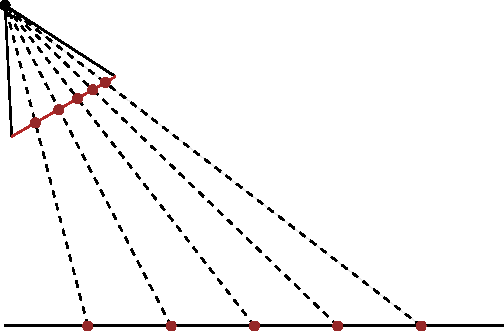
\includegraphics[scale=0.75]{figures/ProjectedGrid_UniformWS.pdf}
\label{fig:subfigprojgrid1}
}
\subtop[Projected Grid]
{
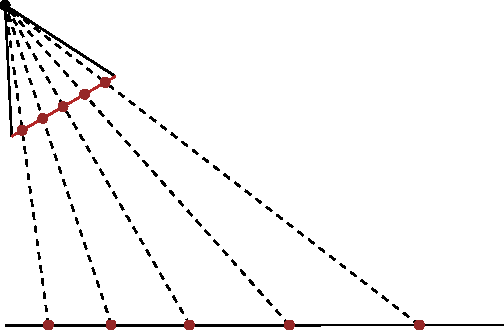
\includegraphics[scale=0.75]{figures/ProjectedGrid_UniformSS.pdf}
\label{fig:subfigprojgrid2}
}
\caption{
\subcaptionref{fig:subfigprojgrid1}
A uniform grid in world space, its projection onto the image plane is not
uniformly spaced though.
\subcaptionref{fig:subfigprojgrid2}
A uniform grid on the image plane, its associated world space positions
are not uniformly spaced.
}
\label{fig:dprojectedgrid}
\end{figure}
%
With all the ocean data synthesized, we may proceed to actually visualize it.
First and foremost we need to take care of the mesh representation of the ocean
surface.
We have already seen that the ocean surface requires a meshing scheme which is
able to automatically adapt to highly distinct viewing situations, such as
closeups of the water surface as well as views with the ocean spanning to the
horizon.
Based on these criteria, we chose to employ the projected grid
~\citep{Hinsinger:2002,thesis:johanson}. The projected grid is based on a
simple concept: to achieve a uniform distribution of detail on the image plane,
a uniformly spaced grid is created in post-perspective space, transformed to
world space and projected onto the $y=0$ plane, see
Figure~\ref{fig:dprojectedgrid}.
Thus, we have constant memory consumption, as the resolution of the grid in
screen space is constant, and we have adaptive level of detail, because all
screen space grid points are projected to points inside the view frustum,
independent of the actual viewing situation. After the vertices have been
projected onto the $y=0$ plane, they are displaced vertically and horizontally
by surface elevation $y(\mvec{x},t)$ and displacement $\mvec{D}(\mvec{x},t)$,
respectively. Last, all vertices are projected normally on the screen via the
viewing pipeline.
%
\subsubsection{Ocean Lighting}
%
% \begin{figure}
%  \centering
%  \subtop[Sky]
%  {
%  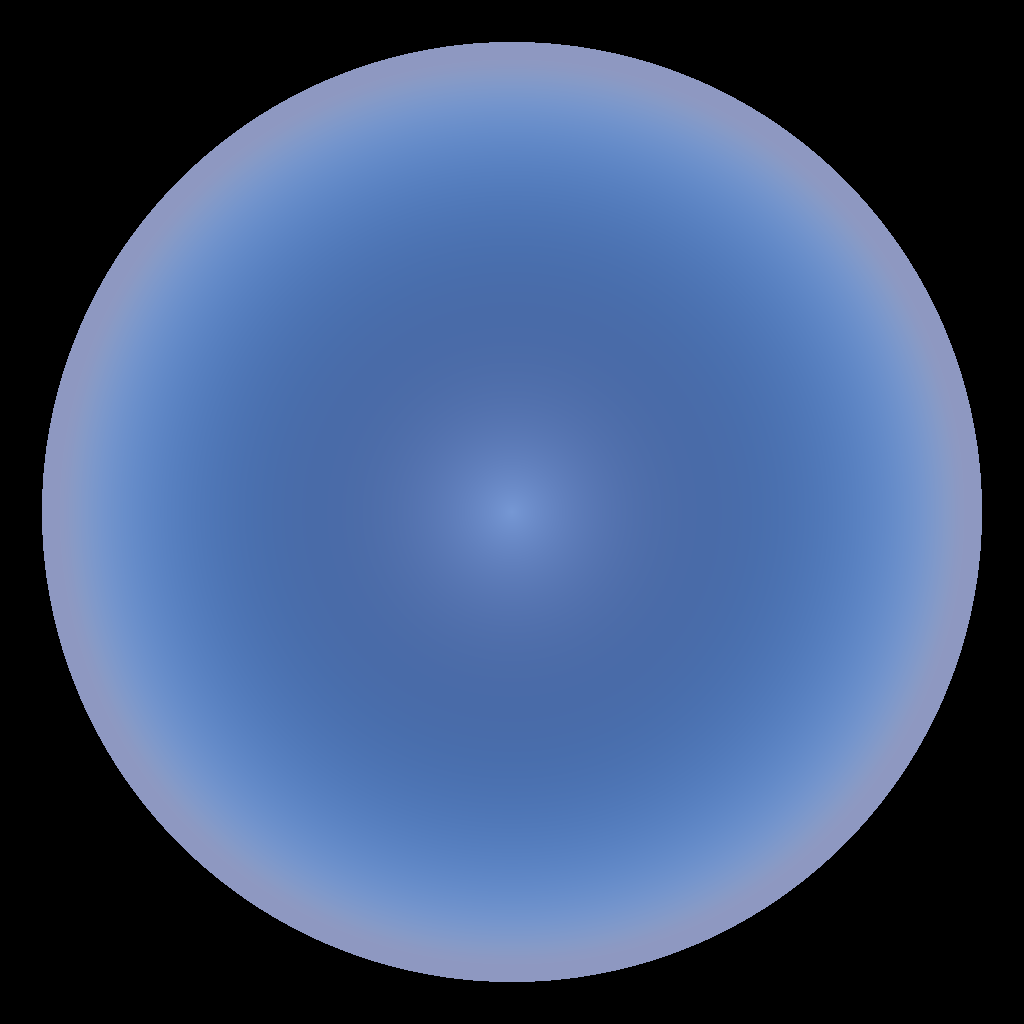
\includegraphics[scale=0.125]{figures/preetham_1.png}
%  }
%  \subtop[Sky + Solar Disc]
%  {
%  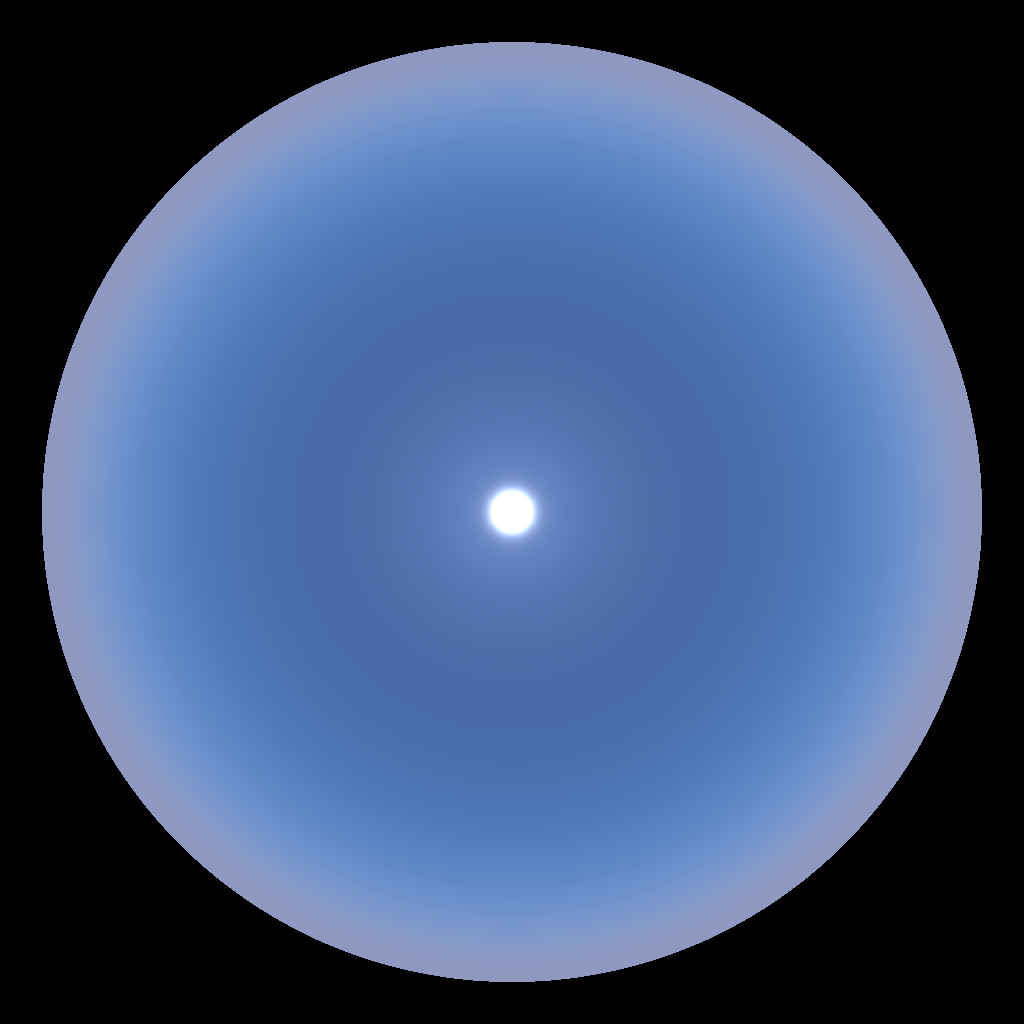
\includegraphics[scale=0.125]{figures/preetham_solar_disk_1.png}
%  }
%  \subtop[Sky + Solar Disc + Irradiance]
%  {
%  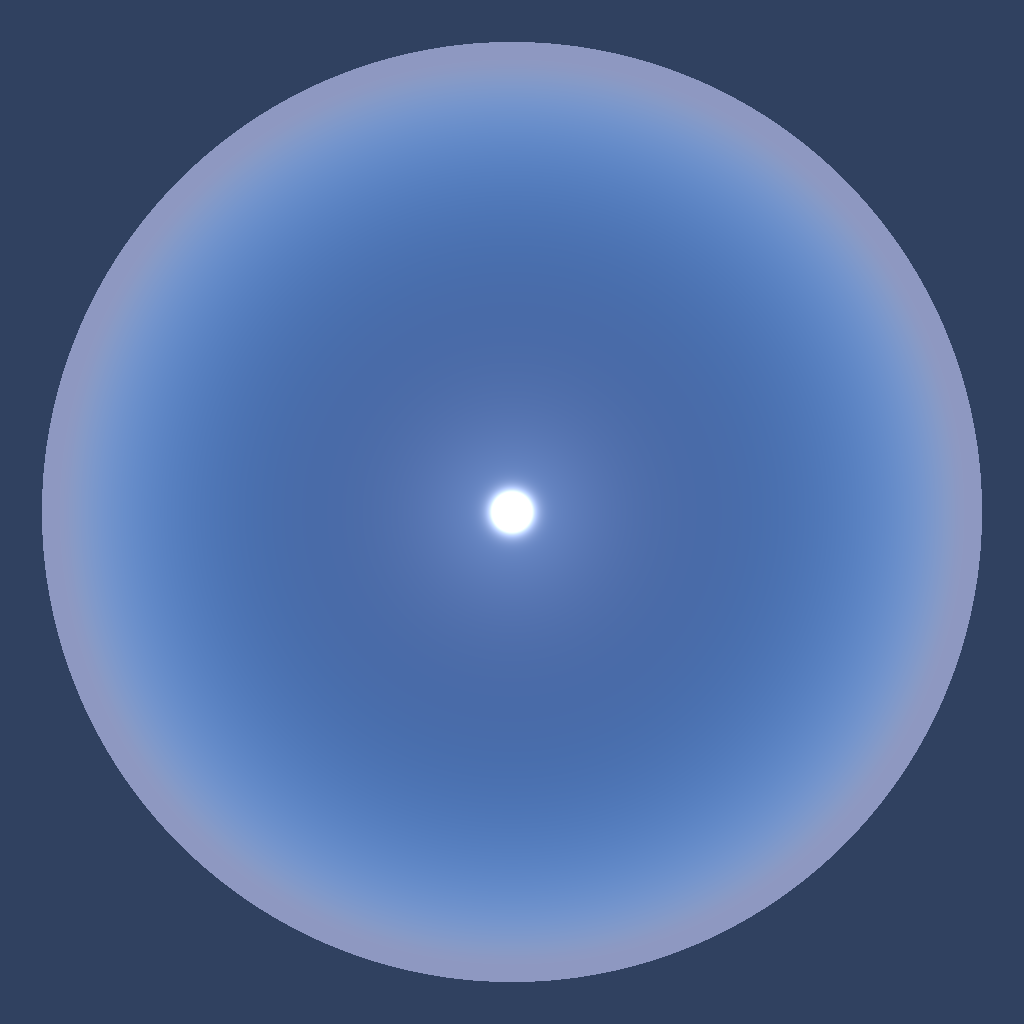
\includegraphics[scale=0.125]{figures/preetham_solar_disk_irradiance_1.png}
%  }
%  \subtop
%  {
%  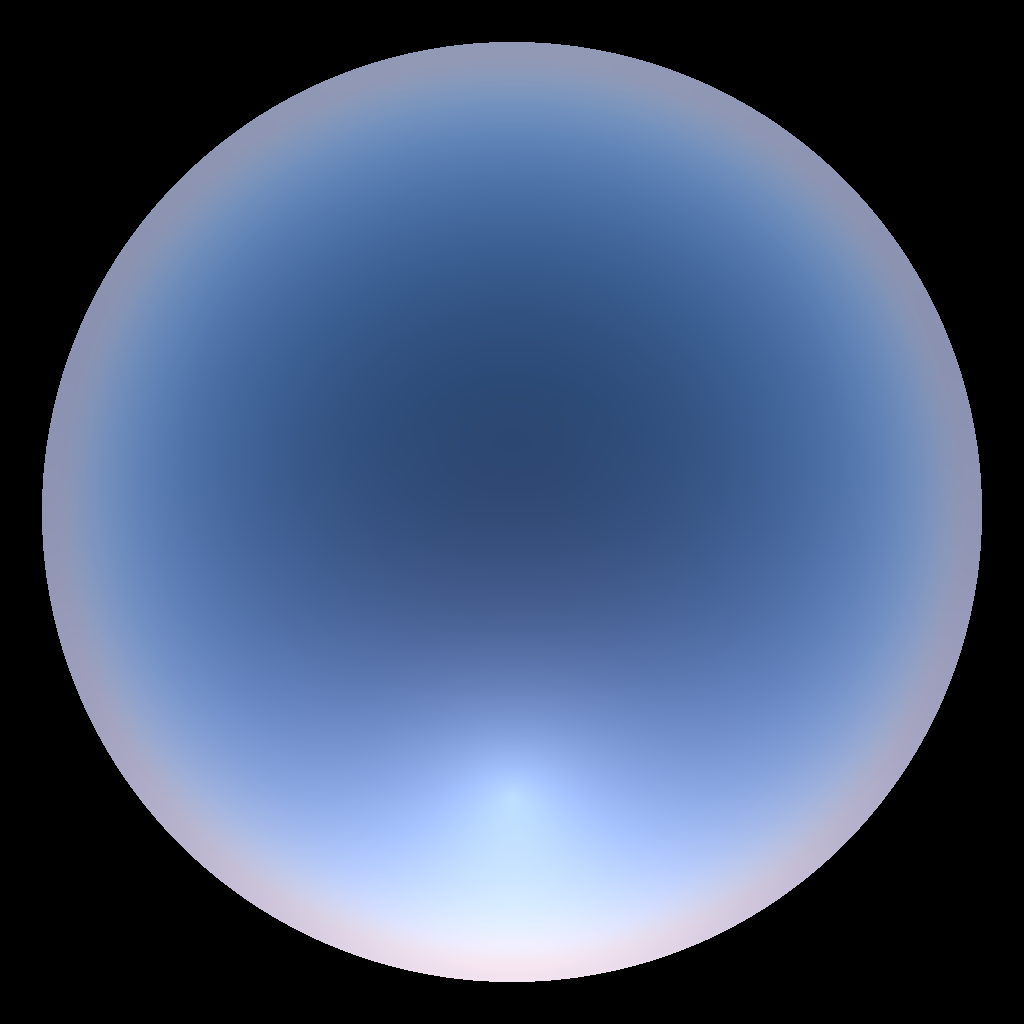
\includegraphics[scale=0.125]{figures/preetham_2.png}
%  }
%  \subtop
%  {
%  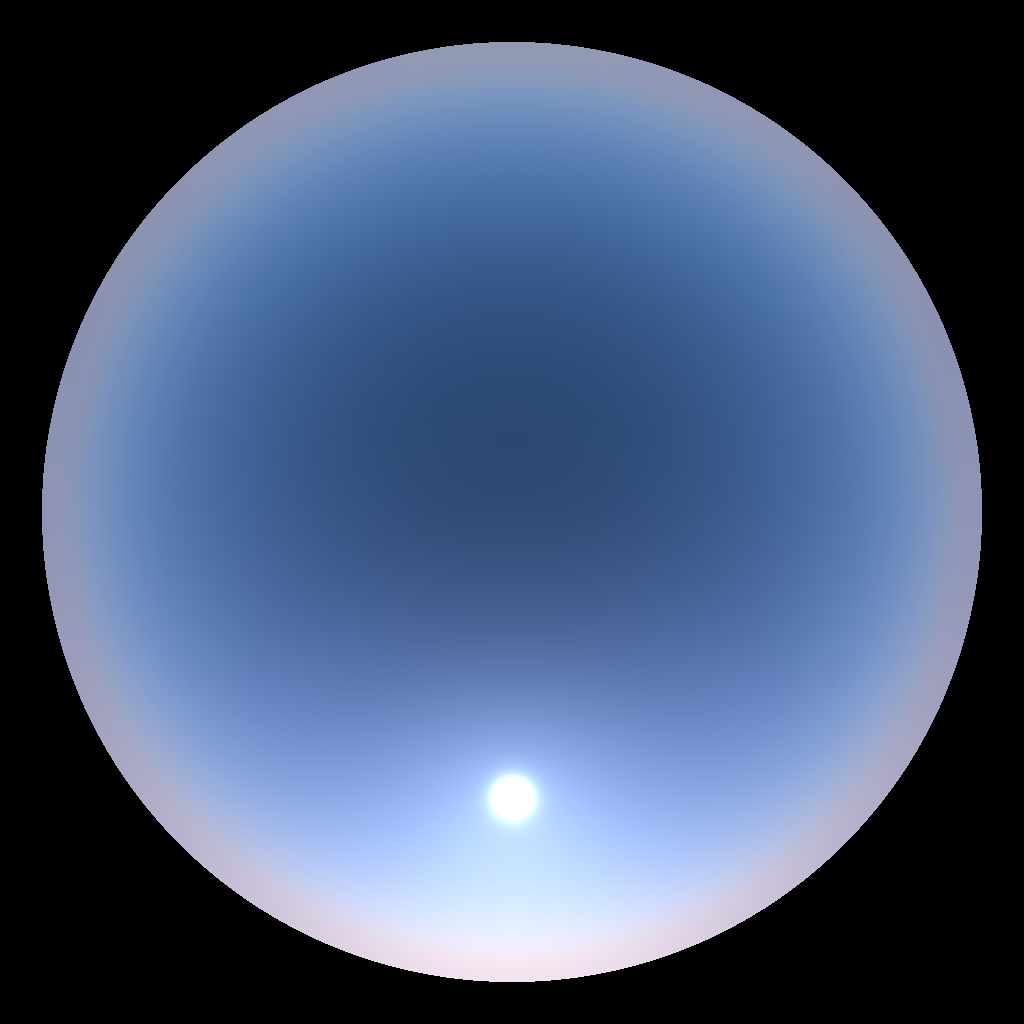
\includegraphics[scale=0.125]{figures/preetham_solar_disk_2.png}
%  }
%  \subtop
%  {
%  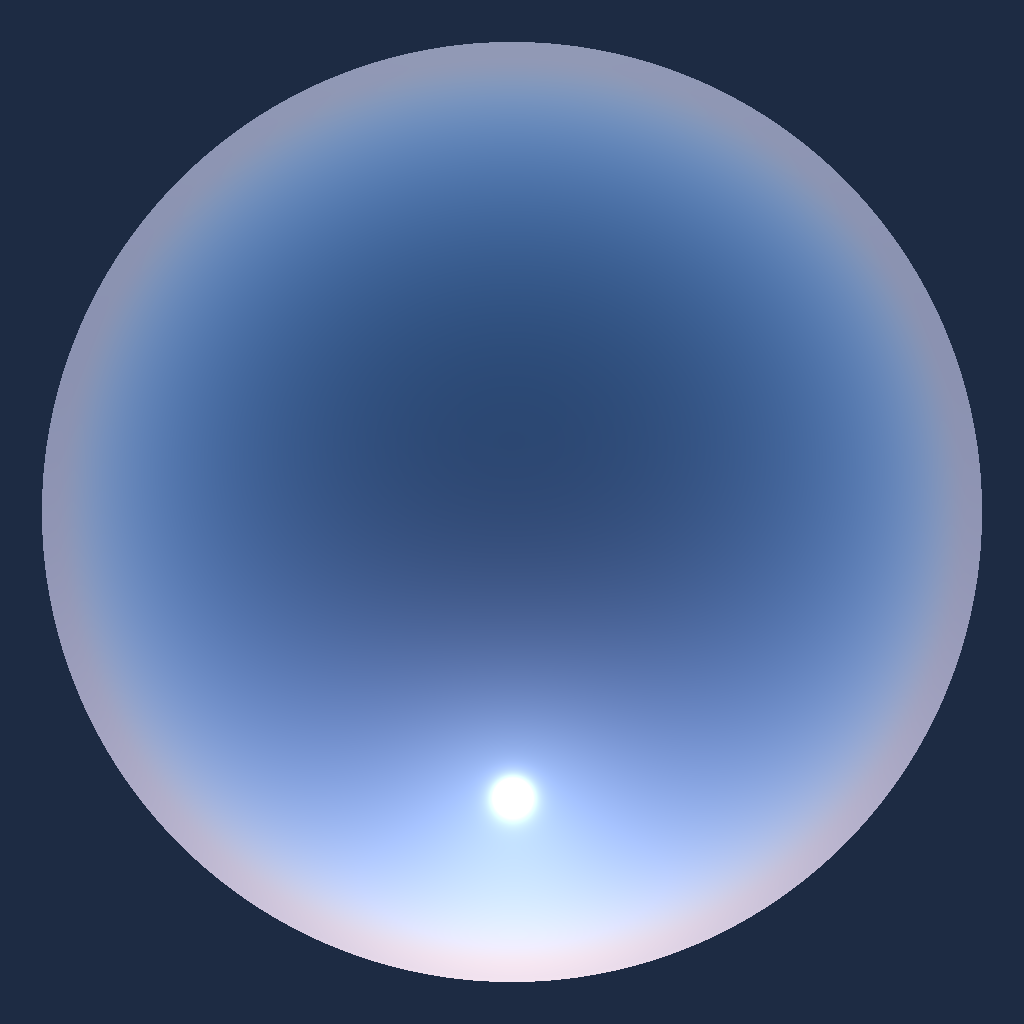
\includegraphics[scale=0.125]{figures/preetham_solar_disk_irradiance_2.png}
%  }
%  \subtop
%  {
%  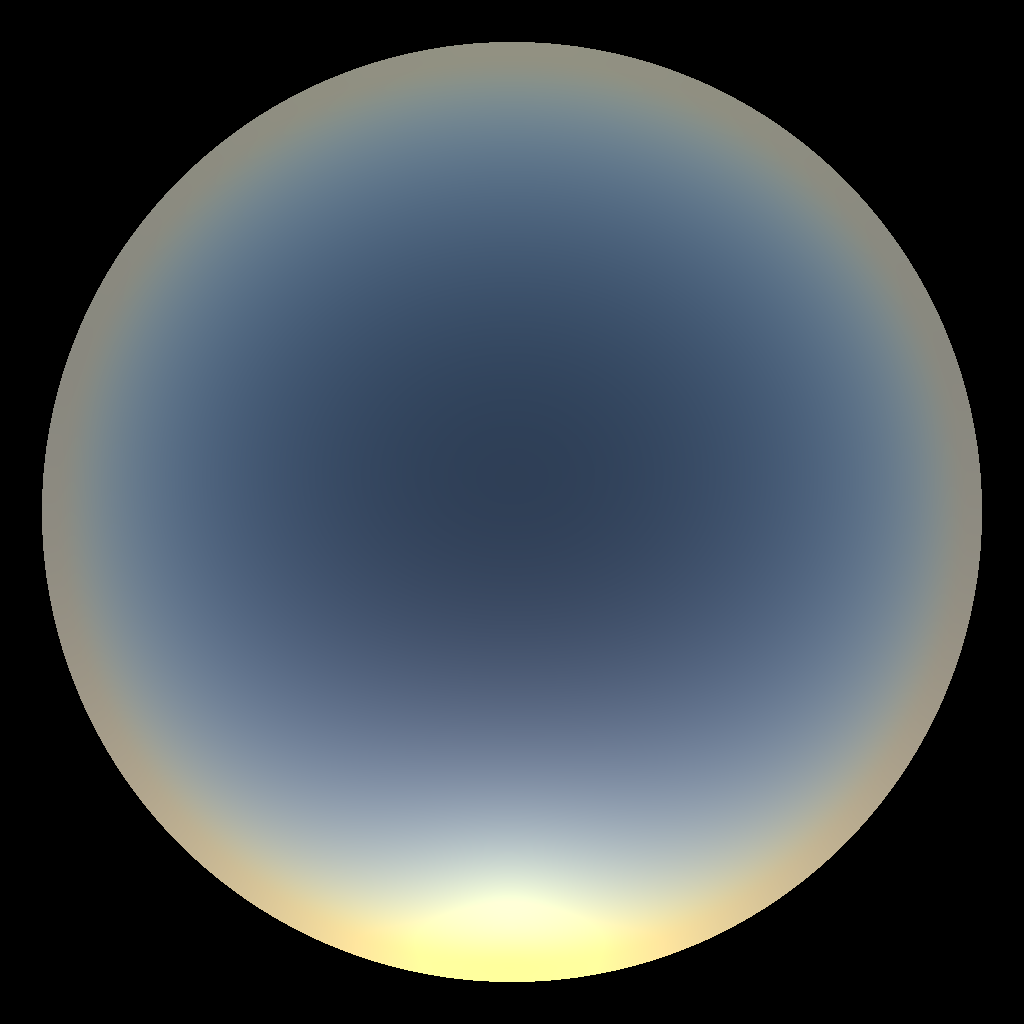
\includegraphics[scale=0.125]{figures/preetham_3.png}
%  }
%  \subtop
%  {
%  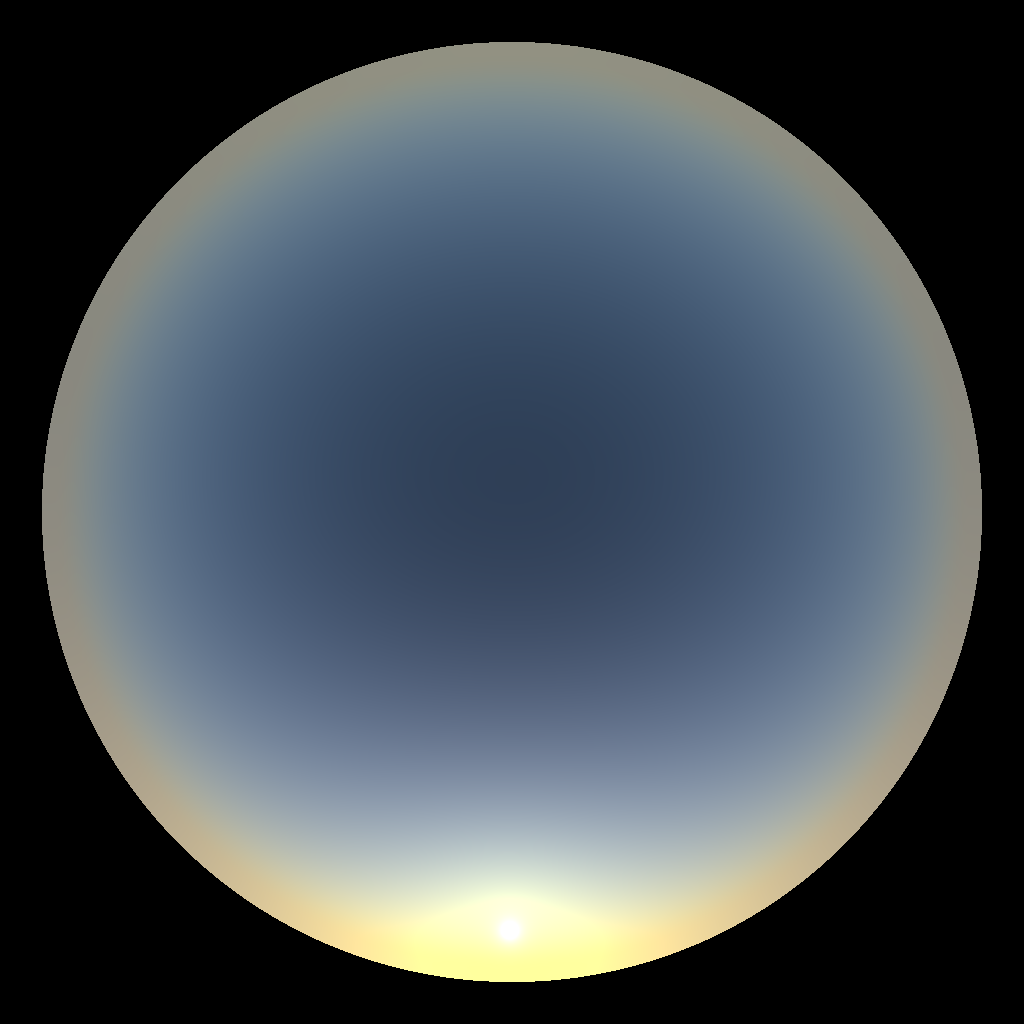
\includegraphics[scale=0.125]{figures/preetham_solar_disk_3.png}
%  }
%  \subtop
%  {
%  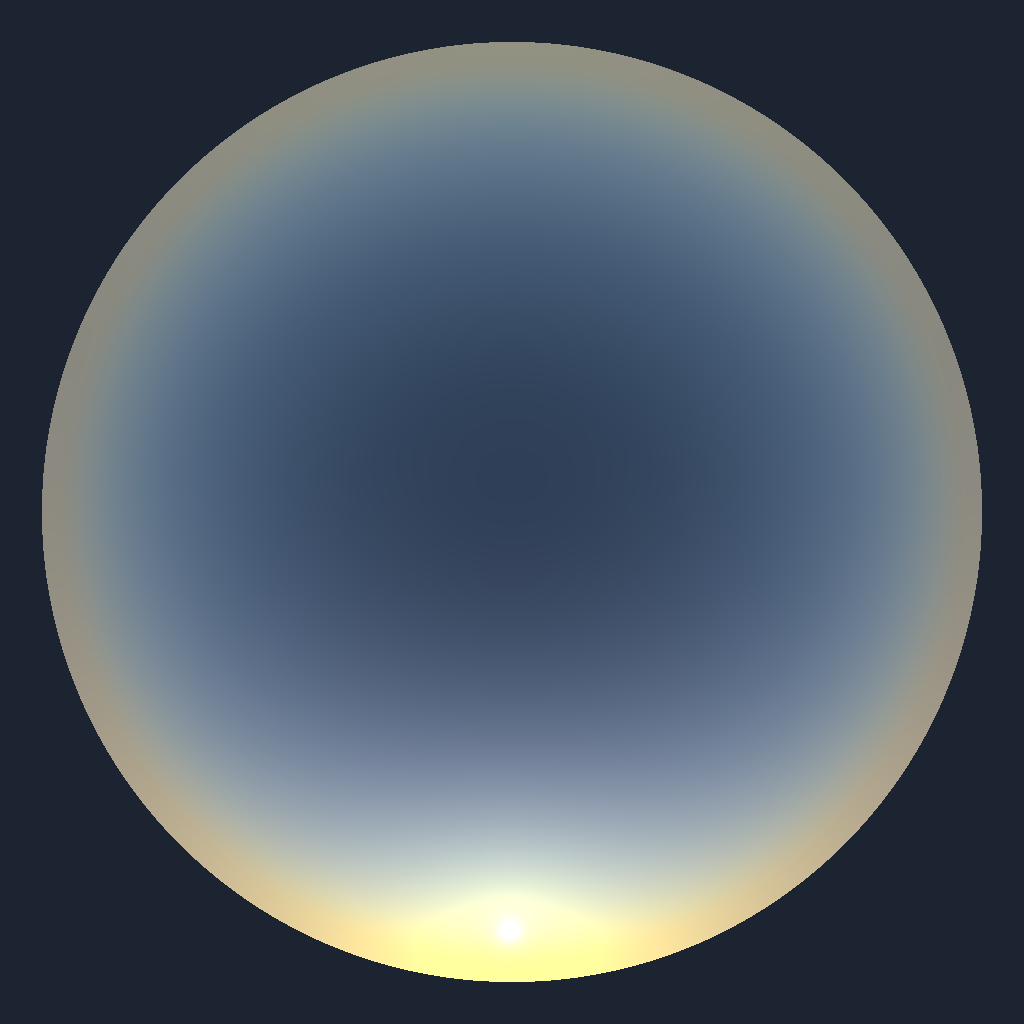
\includegraphics[scale=0.125]{figures/preetham_solar_disk_irradiance_3.png}
%  }
% \caption{Brak.}
% \label{fig:preetham}
% \end{figure}
\begin{figure}
 \centering
 \subtop[$\theta_{sun} = \ang{0}$]
 {
 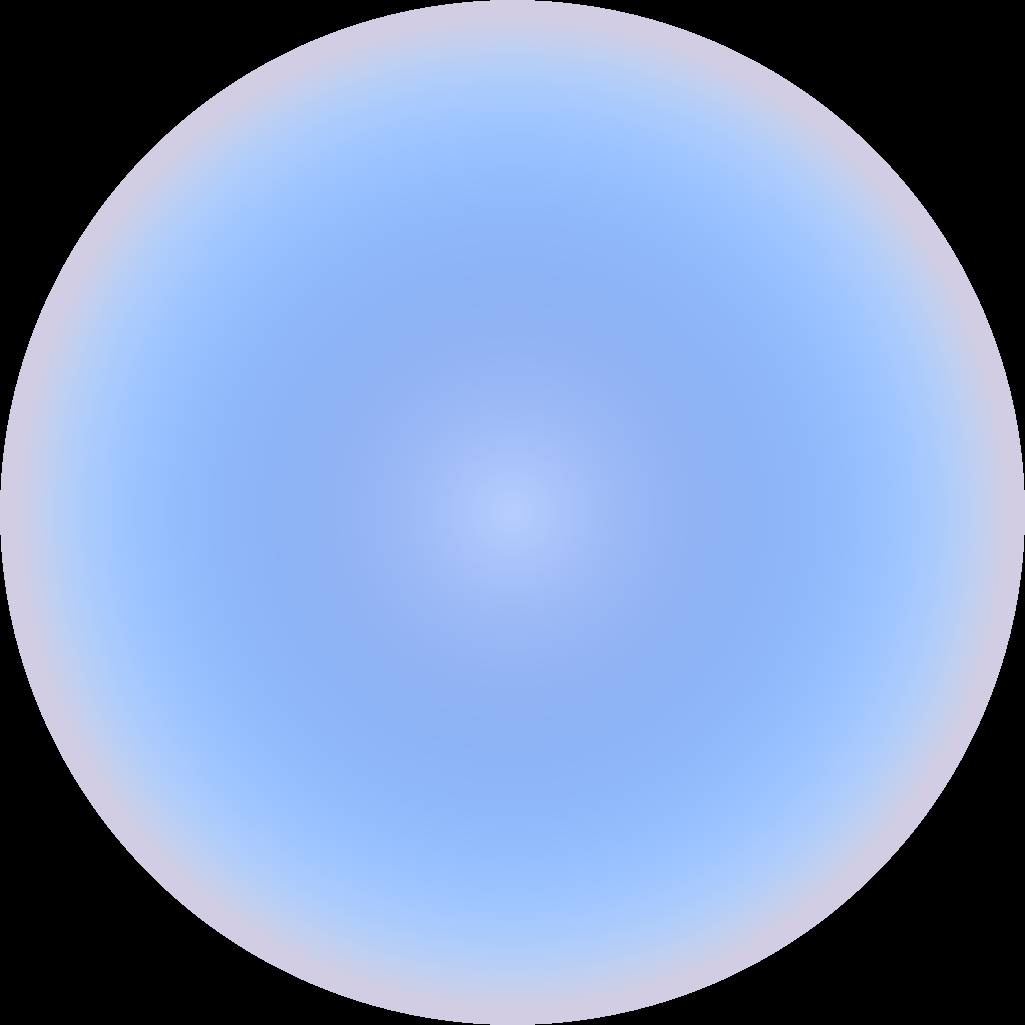
\includegraphics[scale=0.125]{figures/preetham_sRGB_D65_turbidity_2_thetaSun_0.png}
 }
 \hfill
 \subtop[$\theta_{sun} = \ang{30}$]
 {
 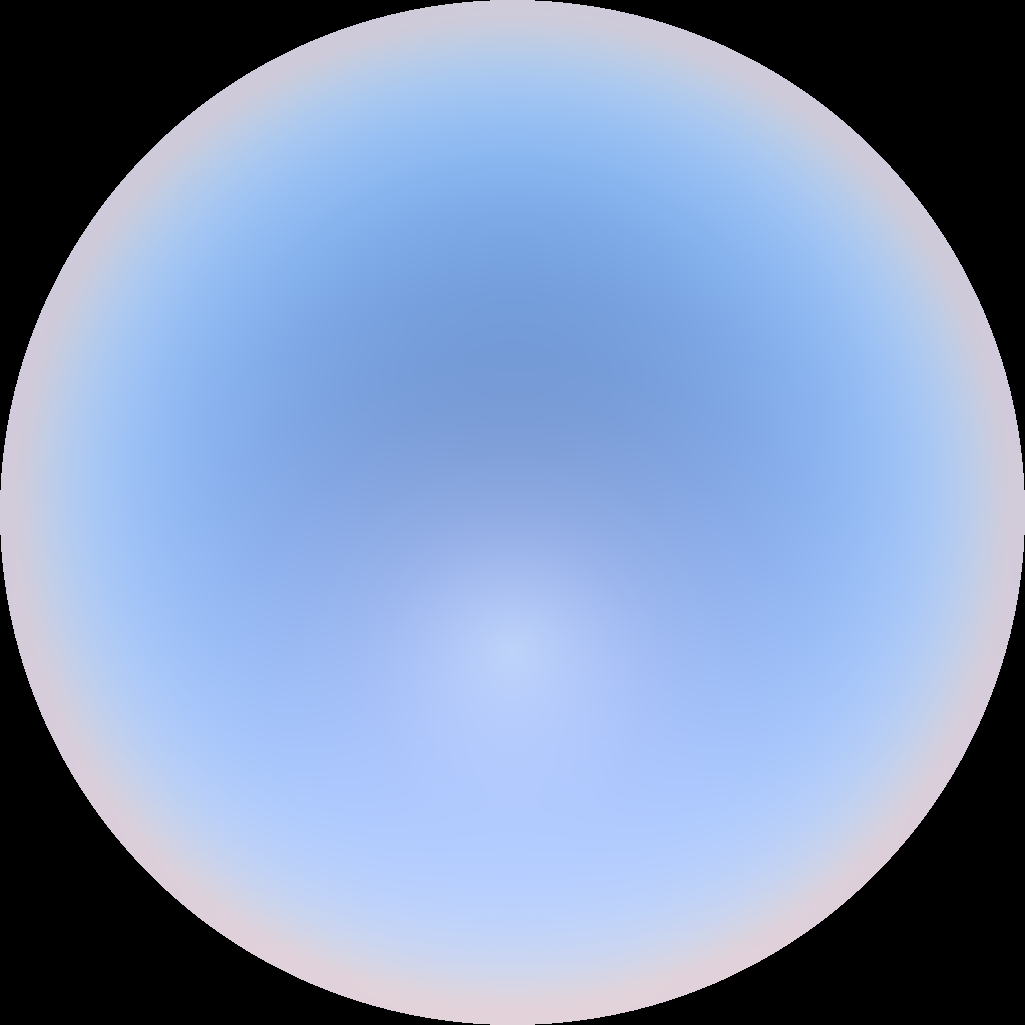
\includegraphics[scale=0.125]{figures/preetham_sRGB_D65_turbidity_2_thetaSun_30.png}
 }
 \hfill
 \subtop[$\theta_{sun} = \ang{60}$]
 {
 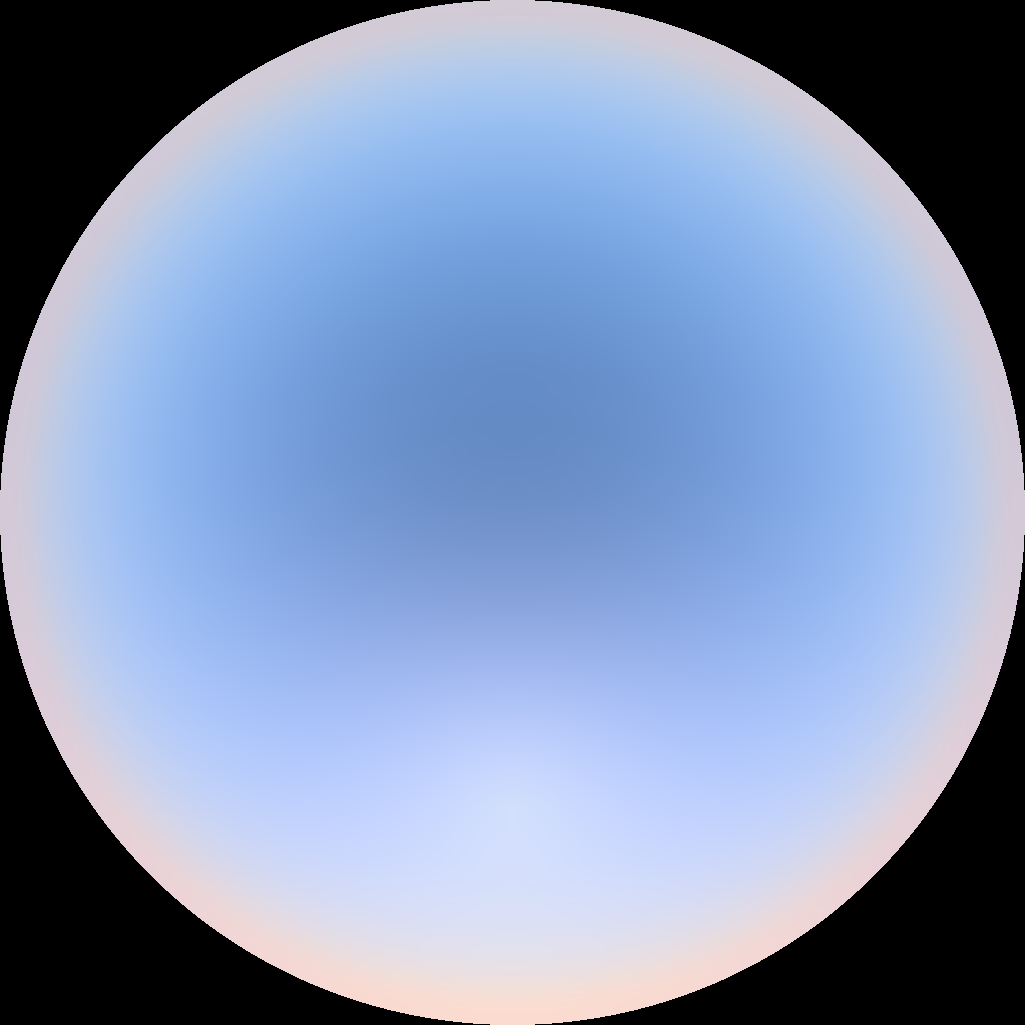
\includegraphics[scale=0.125]{figures/preetham_sRGB_D65_turbidity_2_thetaSun_60.png}
 }
 \hfill
 \subtop[$\theta_{sun} = \ang{90}$]
 {
 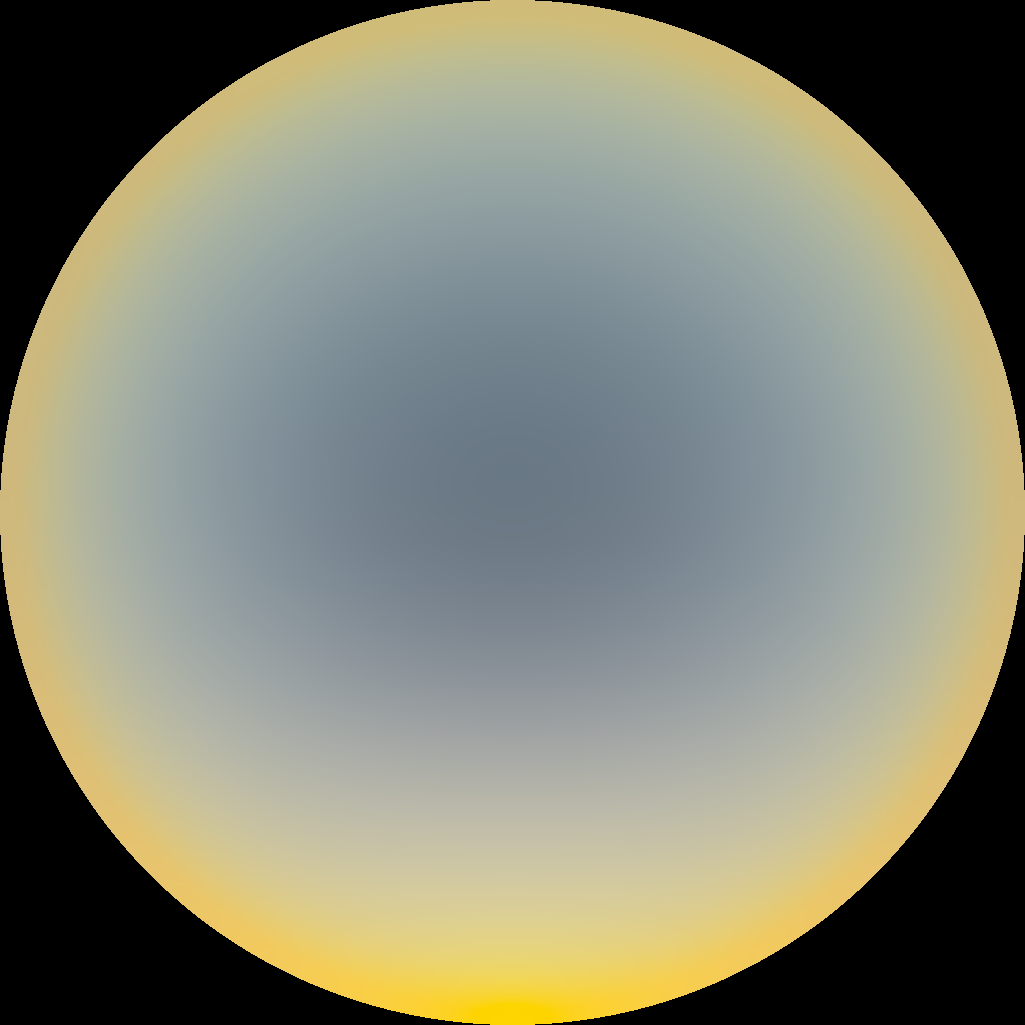
\includegraphics[scale=0.125]{figures/preetham_sRGB_D65_turbidity_2_thetaSun_90.png}
 }
 \subtop
 {
 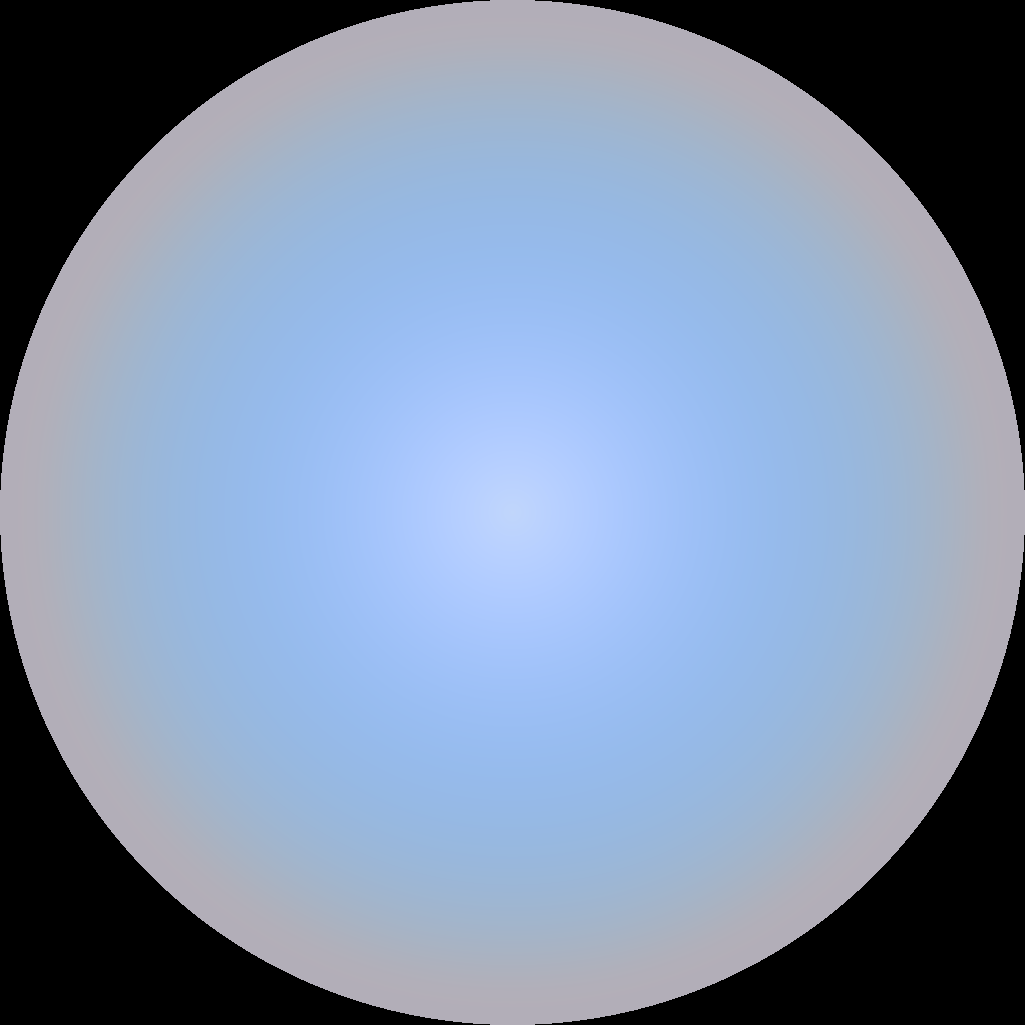
\includegraphics[scale=0.125]{figures/preetham_sRGB_D65_turbidity_4_thetaSun_0.png}
 }
 \hfill
 \subtop
 {
 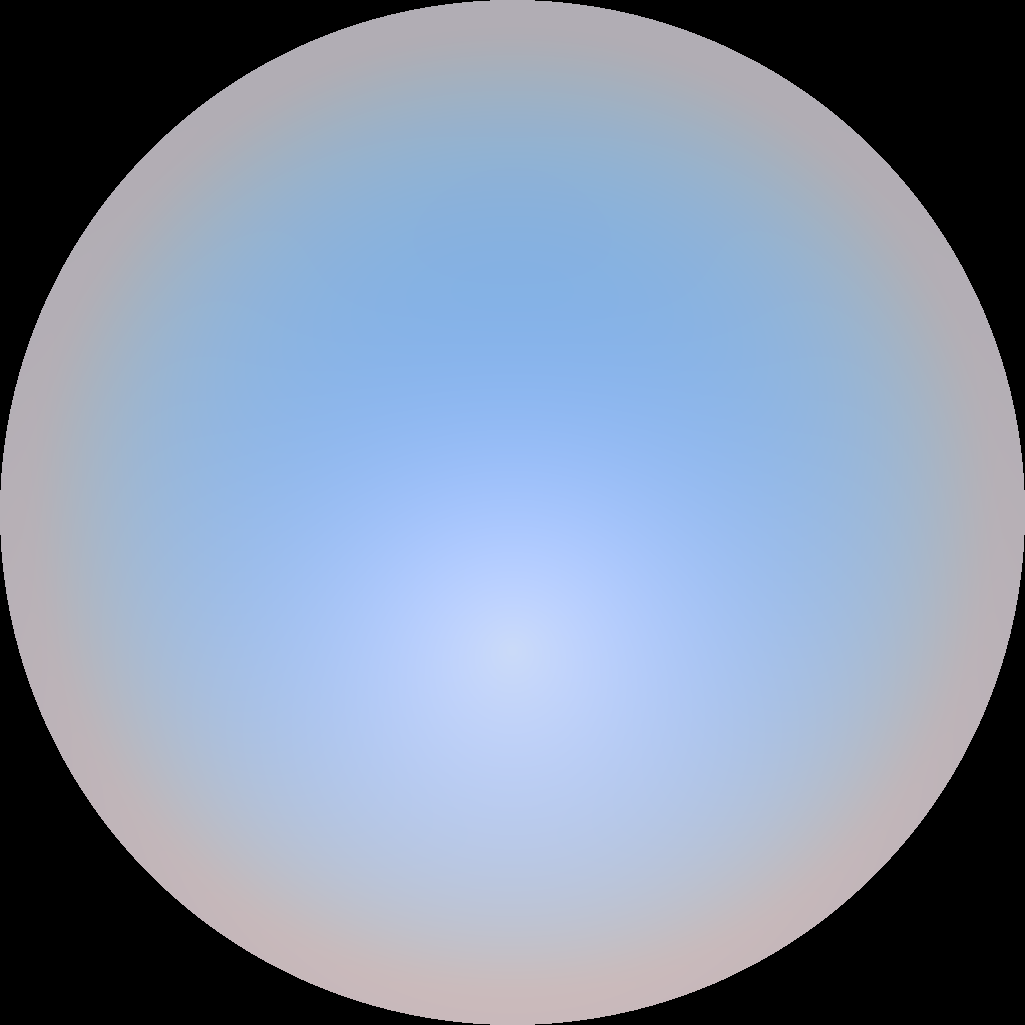
\includegraphics[scale=0.125]{figures/preetham_sRGB_D65_turbidity_4_thetaSun_30.png}
 }
 \hfill
 \subtop
 {
 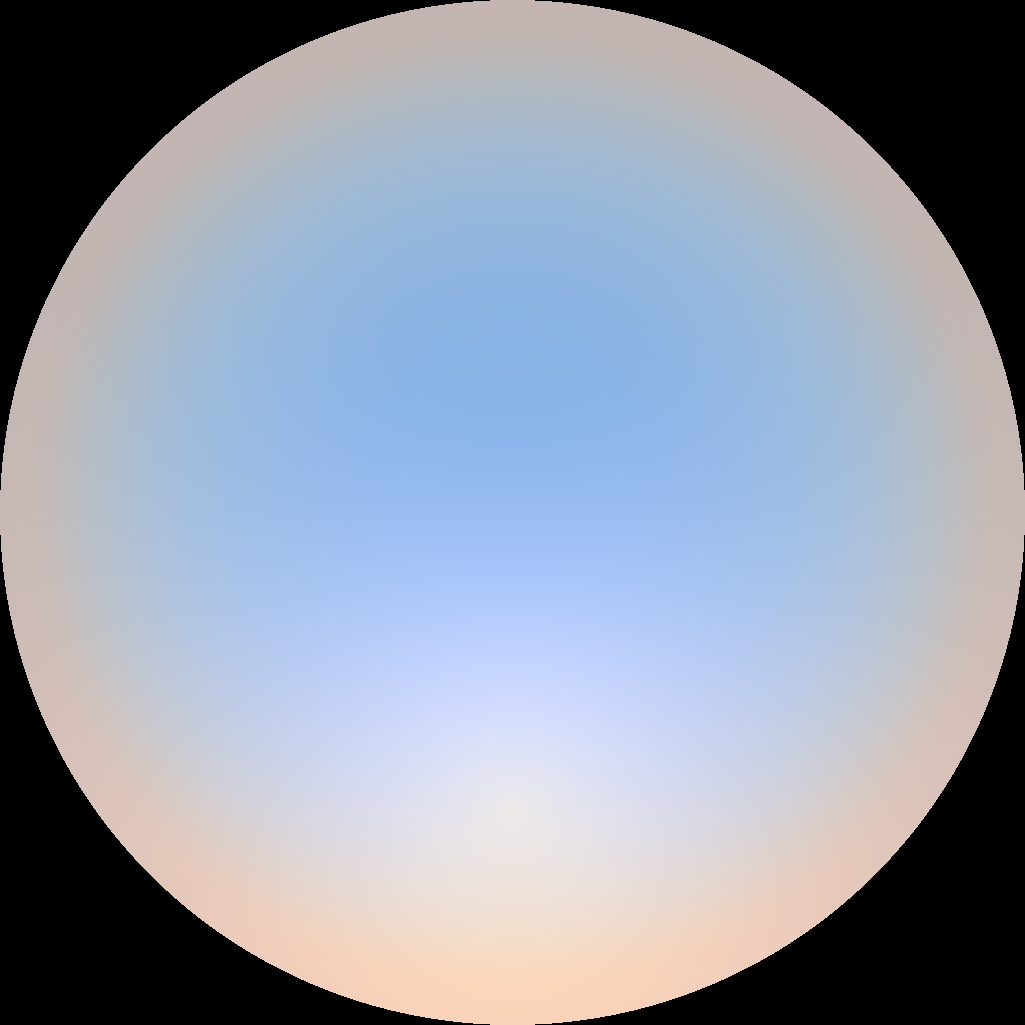
\includegraphics[scale=0.125]{figures/preetham_sRGB_D65_turbidity_4_thetaSun_60.png}
 }
 \hfill
 \subtop
 {
 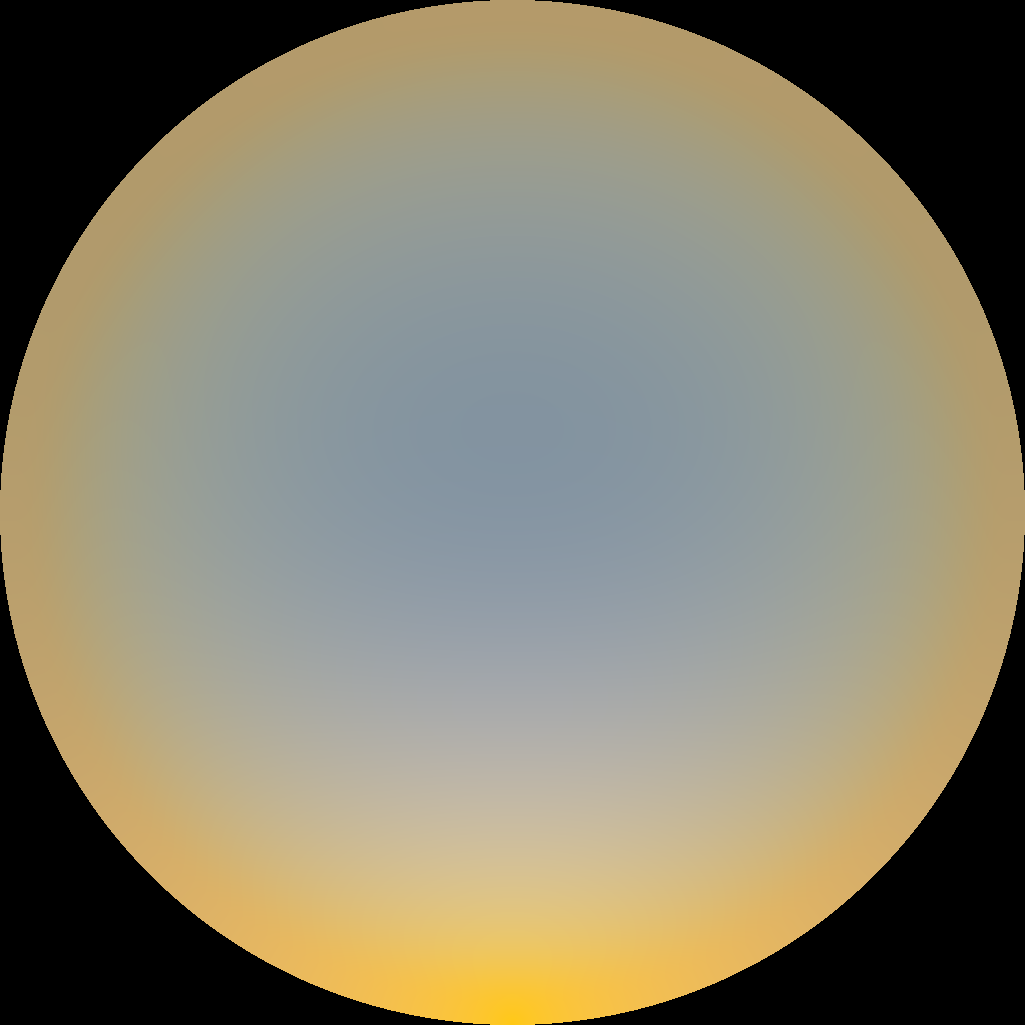
\includegraphics[scale=0.125]{figures/preetham_sRGB_D65_turbidity_4_thetaSun_90.png}
 }
 \subtop
 {
 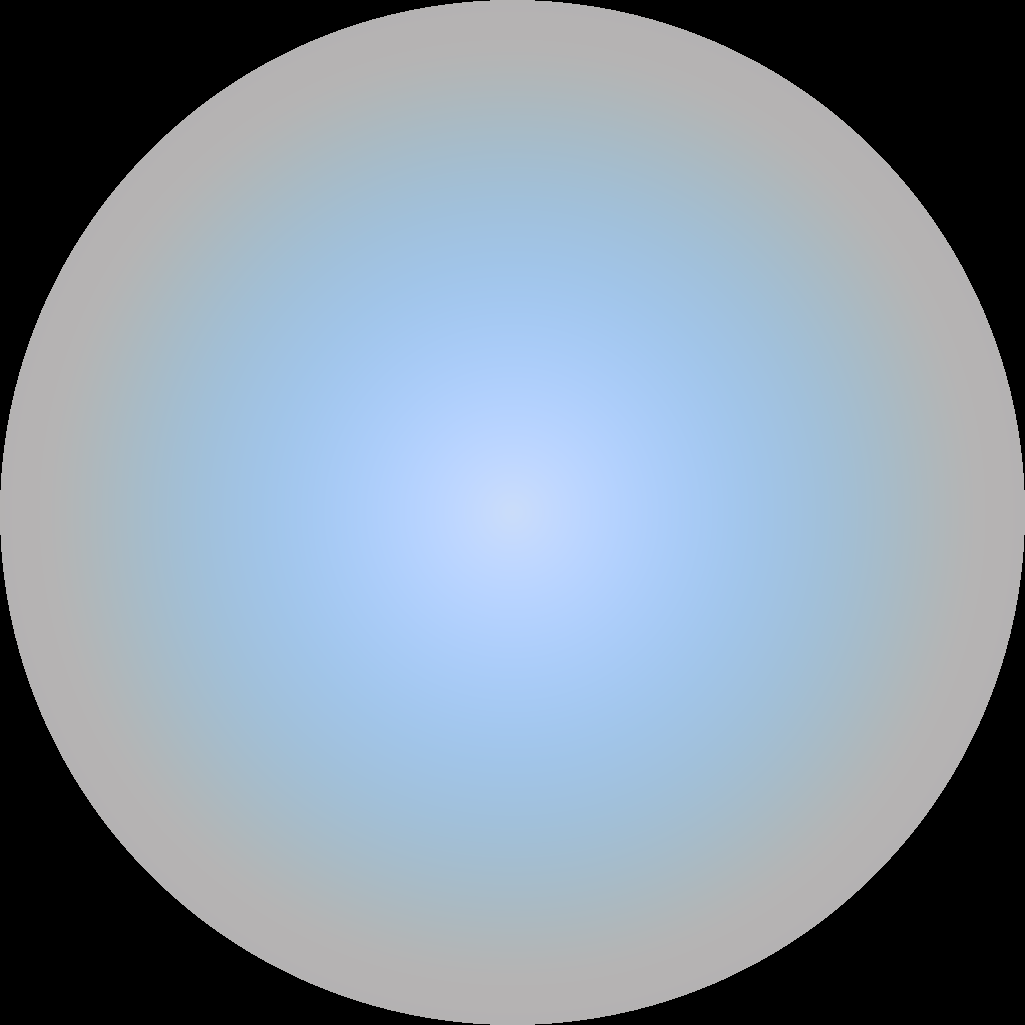
\includegraphics[scale=0.125]{figures/preetham_sRGB_D65_turbidity_6_thetaSun_0.png}
 }
 \hfill
 \subtop
 {
 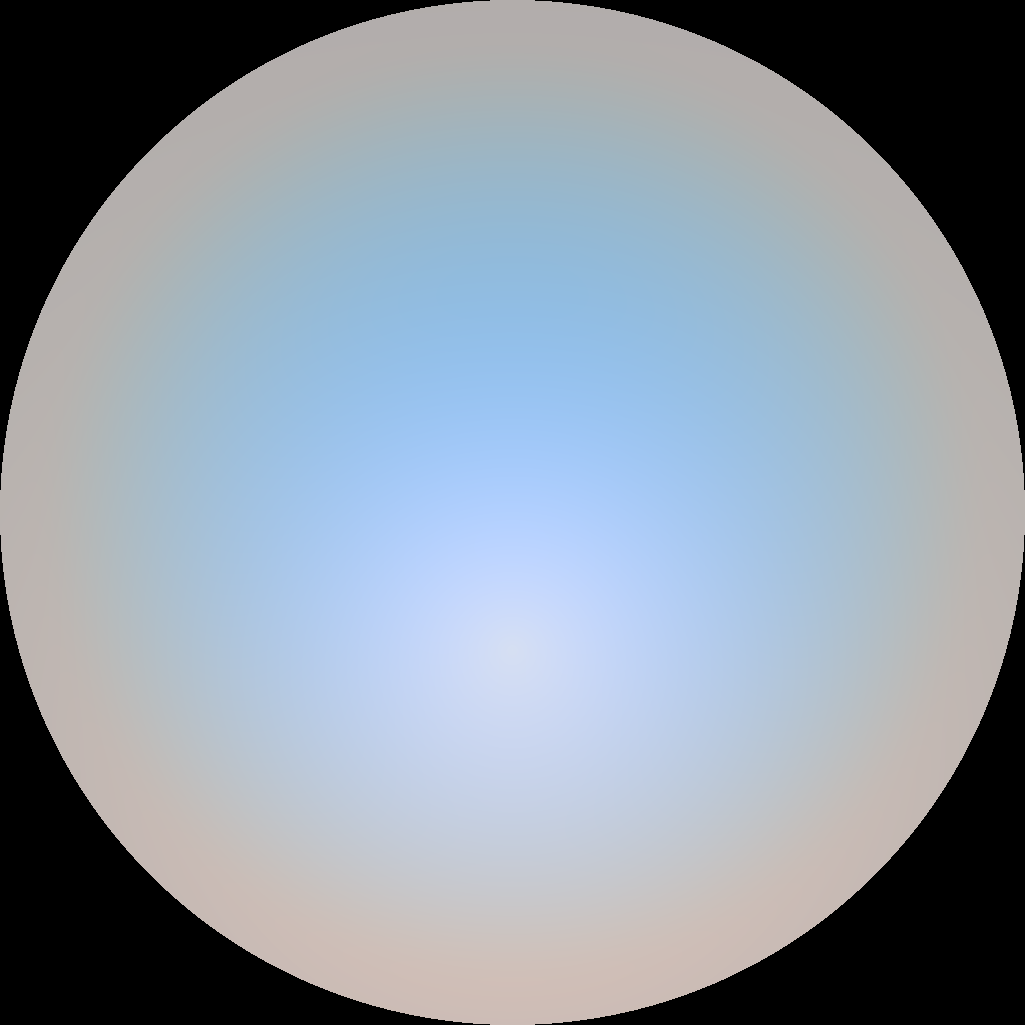
\includegraphics[scale=0.125]{figures/preetham_sRGB_D65_turbidity_6_thetaSun_30.png}
 }
 \hfill
 \subtop
 {
 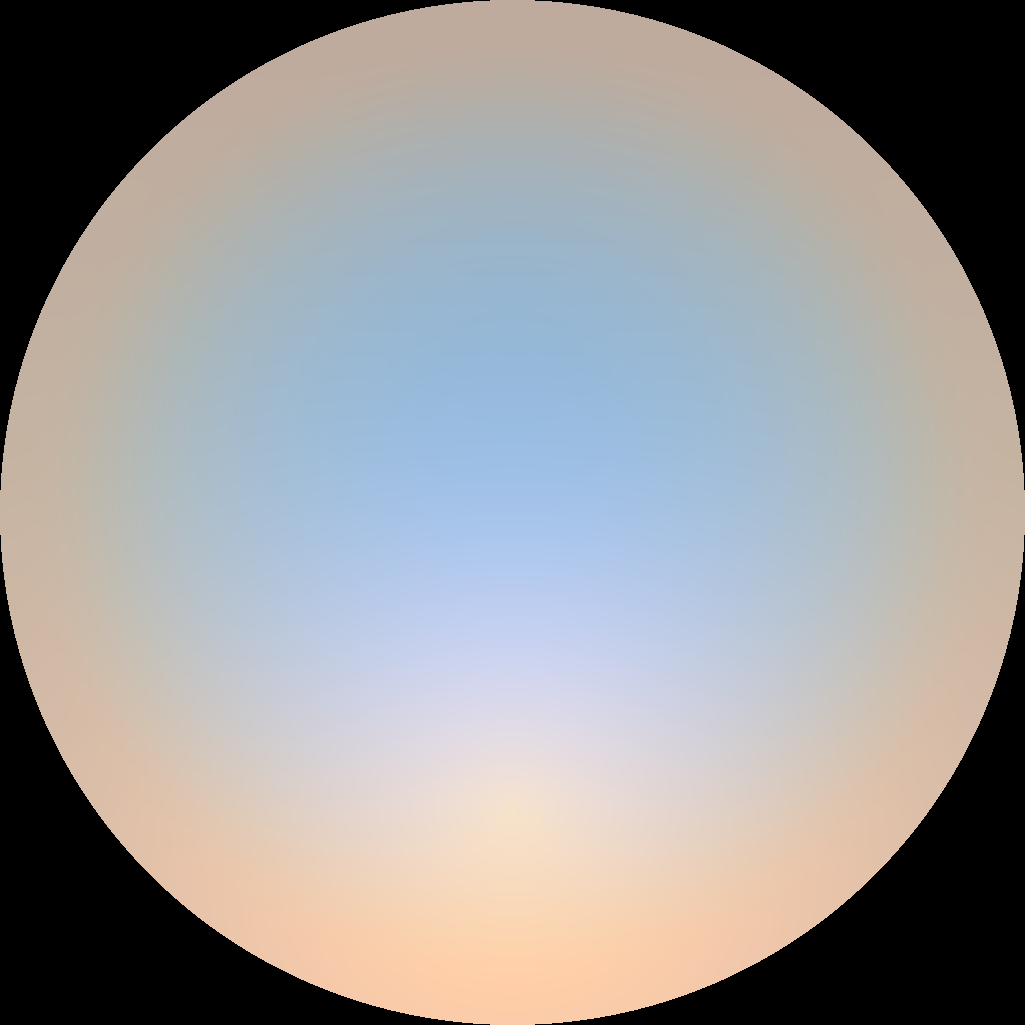
\includegraphics[scale=0.125]{figures/preetham_sRGB_D65_turbidity_6_thetaSun_60.png}
 }
 \hfill
 \subtop
 {
 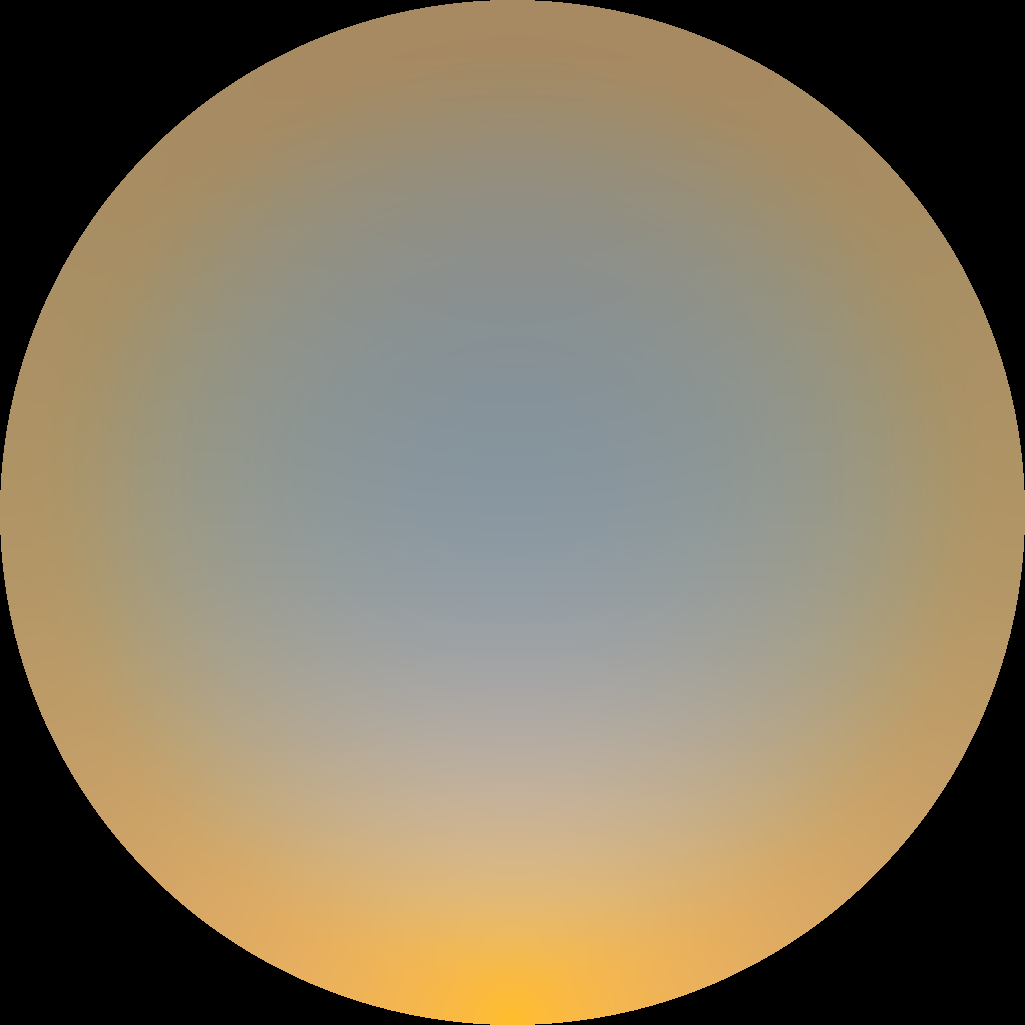
\includegraphics[scale=0.125]{figures/preetham_sRGB_D65_turbidity_6_thetaSun_90.png}
 }
\caption{
Example instances of the Preetham skylight model: the solar zenith angle
$\theta_{sun}$ increases from left to right, turbidity $T$ increases from top
to bottom.
}
\label{fig:preetham}
\end{figure}
%
Now that we have dealt with the ocean surface mesh, we may move on to the next
aspect of ocean surface rendering, namely the illumination of the water surface.
We chose to implement the illumination model introduced by
\citet{article:oceanlighting} for three reasons. First, it gives visually
pleasing as well as convincing results. Second, in step with our work,
it is tailored to the deep water of the open ocean. Third, it has been adapted by
\citet{misc:oceanlightingfft} in such a way, that the wave energy spectrum has
become an integral part of the lighting model itself.

The lighting term for the water surface, as presented by
\citeauthor{article:oceanlighting} consists of three parts:
reflected light from the sun, reflected light from the sky dome, and refracted
light from the water. The latter term describes the fraction of light from
the sun and sky which has entered the water due to refraction, and leaves it
again due to multiple scattering.
%Because we are in deep water,
%\citeauthor{article:oceanlighting} assume that no light which has entered the
%water body is reflected from the sea bed back to the water surface.
To model the sky dome and the sun \citeauthor{article:oceanlighting} employ the
work of \citet{Bruneton:2008}, where the latter compute the interaction of
light and the atmosphere in its entirety. We, on the other hand, chose not to
extend the scope of this thesis any further with such a complex technique, and
therefore opted for the well-established work of \citet{Preetham:1999}, which
is easy to implement and requires no preprocessing steps.
The Preetham skylight model, as presented in \citet[Section 3.1]{Preetham:1999},
takes only two parameters: one, the position of the sun on the hemisphere, and two,
the haziness of the atmosphere i.e. turbidity.
Figure~\ref{fig:preetham} depicts the effect of the two parameters on
the resulting sky dome.
With the skylight taken care of, we may turn towards the sunlight. We assume
the sun to be a directional light source, which is uniform in color and
intensity for the entire scene. \citet[Section 3.2]{Preetham:1999} gives us
intensity and color of the sunlight based on the position of the sun, where
the result is consistent with the corresponding Preetham skylight.
%That is, because 
%\citeauthor{article:oceanlighting} employ an approximation of the BRDF presented
%by \citet{Ross:2005}, where said BRDF is specifically tailored to the
%statistical properties of ocean surfaces. And we have seen in
%Section~\ref{sec:random_sea} that the wave spectrum itself is a statistical
%description of the ocean surface, and thus may provide all data the Ross
%BRDF requires.
%
%which has been adapted for wave spectra by
%\cite{misc:oceanlightingfft}. \citeauthor{article:oceanlighting} employ
%an approximation of the BRDF presented by \citet{Ross:2005}, where said BRDF is
%specifically tailored to the statistical properties of ocean surfaces. And since
%the wave spectrum itself represents a statistical description of the ocean surface,
%it fits very well with said BRDF.
%
%in because it gives believable as well as
%visually pleasing results. Moreover, it has not only been adapted to work
%with a wave spectrum \citep{misc:oceanlightingfft}, the wave spectrum itself
%represents an integral part of the illumination model.

%\citet{article:oceanlighting} augment the work of \citeauthor{Hinsinger:2002} in
%various areas, the most prominent improvement being an adaptive lighting scheme.
%The latter is based on a hierarchical representation which combines geometry,
%normals and a BRDF~\citep{Ross:2005}, where the BRDF is specifically tailored to
%the statistical properties of ocean surfaces. Based on distance from the viewer,
%the algorithm transitions seamlessy from lighting computed with geometry and per
%pixel normals to lighting computed based solely on the statistical distribution
%of ocean surface slopes as modeled by the BRDF, see Figure~\ref{fig:bruneton:transitions}.
%To save computation time for vertex positions, wavetrains are filtered according
%to the size of their associated projected grid cell in world space.
%For the gradient computation in the pixel shader there is an additional step,
%where wavetrains are filtered according to the projected size of the current pixel
%in world space. In addition, \citeauthor{article:oceanlighting} show the
%integration of the BRDF by \citeauthor{Ross:2005} into the computation of
%all necessary lighting terms, namely the reflected light from the sun and from
%the skydome, and the refracted light from the water, as seen in
%Figure~\ref{fig:bruneton:lightingterms}.
%
%\citet{misc:oceanlightingfft} combines the adaptive lighting scheme
%from \citet{article:oceanlighting} with an ocean surface synthesized
%from the wave spectrum presented in~\citet{article:Elfouhaily1997}.
%Wave heights, gradients, as well as the horizontal displacements
%required for the choppy wave algorithm by \citet{course:simulatingocean}
%are computed entirely on the GPU. In an additional step,
%\citet{article:whitecaps} add whitecaps to the ocean lighting model,
%see Figure~\ref{fig:dupuy:whitecaps}.
%
%At this point we make a number of assumptions about the interaction of light
%with the ocean surface, which in part are attributed to the fact that we concern
%ourselves exclusively with deep water. First, the water is deep, therefore no
%light is reflected from the bottom of the ocean back to the surface. Second,
%there are no light sources within the water body.
%
%We concern ourselves only with deep water, allowing us to make a number of
%assumptions about the interaction of light with the water body.
%We concern ourselves only with deep water, therefore we may assume no light is
%reflected from the bottom of the ocean to the ocean surface. It follows that
%the only light exiting the ocean surface from within has previously entered the
%water body via refraction, and leaves it due to scattering.
%Deep water, no light reflected from the ground, only scattering allows for refracted light to reach the surface. Therefore, the appearance of deep water depends largely on the part of the
%incoming light that gets reflected. And most of the incoming light consists of
%direct sunlight and sunlight inscattered via the sky. Therefore we are in need
%of a skylight model. We chose to implement the Preetham Skylight model
%\cite{Preetham:1999}.
\subsubsection{Whitecaps}
The ocean lighting scheme by \citet{article:oceanlighting} does not account for
the breaking of waves on the open ocean. Neither the geometric deformations,
nor the changes in reflectance caused by foam and spray, so called
whitecaps, are incorporated in their model. \citet{article:whitecaps},
on the other hand, extend the work of \citet{misc:oceanlightingfft}
to include whitecaps.
Their contribution is an optimized algorithm to compute for each pixel the
coverage caused by whitecaps. Said coverage depends on the amount of self
intersections taking place inside the world space footprint of the pixel on
the ocean surface. With the whitecap coverage at hand,
\citeauthor{article:whitecaps} then proceed to modify the lighting term at each
pixel accordingly.
The aforementioned self intersections are located using the approach by
\citet{course:simulatingocean}, whereas the computation of the whitecap
coverage is based on fast linear prefiltering methods \citep{Bruneton:2012},
allowing it to leverage the hardware accelerated mipmap generator of modern GPUs.

%Their approach is based on the method by
%\citet{course:simulatingocean} to locate self intersections on the ocean
%surface (Section~\ref{sec:self_intersections}). Given the
%location of a self intersection, the reflectance at that surface position may
%be modified to account for foam and spray.
%
%\citeauthor{article:whitecaps} contribute an optimized algorithm to compute
%the whitecap fractional coverage inside a pixel. Said coverage depends on the
%amount of self intersections which take place inside the world space footprint
%of the pixel on the ocean plane. The algorithm is based on fast linear
%prefiltering methods \citep{Bruneton:2012}, allowing it to leverage the
%hardware accelerated mipmap generator on modern GPUs.
%
%We may generate whitecaps whenever the following function gives a result equal
%one:
%\begin{equation}
 %whitecap(\mvec{x},t) = H(\epsilon - det(\mvec{J}(\mvec{x},t)))
%\end{equation}
%where $det(\mvec{J}(\mvec{x},t))$ is the Jacobian determinant of the horizontal
%displacement function $\mvec{y}(\mvec{x},t) = \mvec{x}+u\mvec{D}(\mvec{x},t)$,
%$H$ is the Heaviside function and the variable $\epsilon$ controls the amount of
%breaking. According to Dupuy et al. we may approximate the whitecap fractional
%coverage $W$ inside a pixel as follows:
%\begin{equation}
 %W = \frac{1}{A}\iint\limits_A whitecap(\mvec{x},t)\mathrm{d}\mvec{x}
%\end{equation}
%where $A$ represents the footprint of the pixel on the ocean plane. Dupuy et al.
%contribute an optimized algorithm to compute $W$ per pixel on the GPU. Their
%algorithm is based on fast linear prefiltering methods, allowing it to leverage
%the hardware accelerated mipmap generator on modern GPUs. It requires an
%additional preprocessing step, with the first order partial derivatives of
%displacements $\mvec{D}(\mvec{x},t)$ of all patterns as input. The output
%consists of variables $k_i$ and $k_i^2$ from Equation 7 and 8 in
%\cite{article:whitecaps}, which are used to compute the per-pixel whitecap
%fractional coverage $W$ via Equation 6 in \cite{article:whitecaps}.

% Given the Jacobian determinant $det(\mvec{J}(\mvec{x},t))$ of the horizontal
% displacement function $\mvec{y}(\mvec{x},t) = \mvec{x}+u\mvec{D}(\mvec{x},t)$,
% we may generate whitecaps whenever the following function gives a result equal
% one:
% \begin{equation}
%  whitecap(\mvec{x},t) = H(\epsilon - det(\mvec{J}(\mvec{x},t)))
% \end{equation}
% where $H$ is the Heaviside function and the variable $\epsilon$ controls the
% amount of breaking.

%  Said modification is based on
% the magnitude of the Jacobian determinant $det(\mvec{J}(\mvec{x},t))$ of the
% horizontal displacement $\mvec{x}+u\mvec{D}(\mvec{x},t)$.

\subsubsection{Tonemapping}
Rendering the ocean illuminated by the Preetham sun- and skylight results
in an image with a high dynamic range. For proper display of the image, we
need to map it to the lower dynamic range of a standard monitor by means of
a tonemapping operator. We chose to employ the global tonemapping operator
by \citet[Equation 4]{Reinhard:2002} because it is straightforward to implement
and works well on the class of images our demo application renders.
As the dynamic range of the image may change from frame to frame, we found it
beneficial to emulate the behavior of the temporal luminance adaptation process
of human vision. For simplicity's sake we chose to use the temporal luminance
adaptation algorithm by \citet[Equations 5, 6, 7, 12]{Krawczyk:2005}, which
gives acceptable results and is easily integrated with the global tonemapping
operator by \citeauthor{Reinhard:2002}

%\emph{Note}: For the interested reader we may mention that
%\citet[Equation 1]{Reinhard:2002} is incorrect, for the correct
%version see \citet{Reinhard:2002:erratum}.

%Rendering the Preetham sky and the ocean results in an image with a high dynamic range.
%We need to map said image to the lower dynamic range of a standard monitor, by means
%of a tonemapping operator. We chose Reinhard's global tonemapping operator, see
%Equation 4 in \cite{Reinhard:2002}. It is straightforward to implement and
%works well on the class of images the demo application renders.
%
%In a first step we compute the log-average luminance $\bar L_w$ of the input image.
%Note, that Equation 1 in\cite{Reinhard:2002} is incorrect, see\cite{Reinhard:2002:erratum}.
%The correct form to compute the log-average luminance of an image is as follows:
%\begin{equation}
 %\bar L_w = \exp\left(\frac{1}{N}\sum\limits_{x,y}\log(\delta + L_w(x,y))\right)
%\end{equation}
%where $N$ is the number of pixels in the image, $L_w(x,y)$ is the ''world'' luminance
%for pixel $(x,y)$, and $\delta$ is small positive value to avoid the singularity at
%$\log(0)$. The value of $\bar L_w$ serves as an approximation to the~\emph{key} of
%the scene. The key indicates whether a scene appears subjectively light, normal, or
%dark. Next we define what luminance the log-average luminance is mapped to in the
%result image. We may write:
%\begin{equation}
%\label{eq:luminance_scaling_reinhard}
 %L(x,y) = \frac{a}{\bar L_w}L_w(x,y)
%\end{equation}
%where $L(x,y)$ denotes the scaled luminance, and $a$ represents the value
%$\bar L_w$ is mapped to.
%We may call $a$ the key value, because it controls the key of the resulting image.
%According to Reinhard et. al. for a scene with normal key it is desirable to
%map the log-average luminance to the subjective middle brightness of the
%displayed image, hence to $a=0.18$, where $a$ lies in the interval
%$\interval{0}{1}$. Lower values for $a$ result in a more darker image, higher
%values in a more brighter image. It is in the last step that we actually
%compute the luminance for each pixel of the result image:
%\begin{equation}
%\label{eq:reinhard_operator}
 %L_d(x,y) = \frac{L(x,y)\left(1+\frac{L(x,y)}{L^2_{white}}\right)}{1+L(x,y)}
%\end{equation}
%where $L_{white}$ is the smallest luminance that will be mapped to pure white.
%This formulation brings all luminances $L \leq L_{white}$ within displayable
%range, whereas all luminances $L > L_{white}$ will appear as pure white,
%simulating a simple oversaturation effect.
%
%As luminance conditions may change from frame to frame, we would like to emulate
%the behaviour of the temporal luminance adaptation process of human vision. We
%employ the temporal luminance adaptation algorithm by Krawczyk et. al.
%\cite{Krawczyk:2005}, namely Equations 5, 6, 7 on page three, and Equation 12 on
%page 5. In short, we replace the $\bar L_w$ term in Equation\ref{eq:luminance_scaling_reinhard}
%with a filtered value $\bar L_a$. Based on our notation from above, we may write
%$\bar L_a$ as follows:
%\begin{subequations}
%\begin{align}
 %\bar L_a^{new} &= \bar L_a + (\bar L_w - \bar L_a) (1-e^{-\frac{T}{\tau}}) \\
%\intertext{with}
 %\tau &= \sigma(\bar L_w)\tau_{rod} + (1-\sigma(\bar L_w))\tau_{cone} \\
 %\sigma(L) &= \frac{0.04}{0.04 + L}\\
 %\tau_{rod} &= 0.4\text{s} \\
 %\tau_{cone} &= 0.1\text{s}
%\end{align}
%\end{subequations}
%where $T$ denotes the timestep between two frames, and $\tau$ represents the
%speed of the adaptation process. For further details the reader may consult
%Krawczyk et. al.\cite{Krawczyk:2005}.

%The implementation of the overall tonemapping algorithm is simple: first convert
%each source pixel from RGB to CIE xyY, where the luminance component Y acts as
%the pixel's ''world'' luminance $L_w$. Next, we update the luminance component Y
%according to Equation~\ref{eq:reinhard_operator}, and as a last step convert the
%luminance adjusted xyY color back to RGB and store it in the target. The actual
%colorimetric conversion functions we use are documented in \cite{misc:colorconversion}.
%The log-average luminance $\bar L_w$ is computed for each frame by simple means
%directly on the GPU. We employ a render target the same size as the source image,
%where for each pixel of the source image we compute $\log(\delta + L_w(x,y))$ and
%write it to the render target. Next, we generate the mipmap pyramid for our render
 %target. The highest mipmap level is one pixel in size and gives us
%$\frac{1}{N}\sum\log(\delta + L_w(x,y))$. Hence, we are able to get $\bar L_w$ by sampling
%the highest mipmap level of our render target and then applying $\exp$ on the result.
%Given $\bar L_w$ we are also able to compute the adapted log-average luminance $\bar L_a$.